\documentclass[conference]{IEEEtran}
\IEEEoverridecommandlockouts

\usepackage{cite}
\usepackage{amsmath,amssymb,amsfonts}
\usepackage{algorithm}
\usepackage{algorithmic}
\usepackage{graphicx}
\usepackage{textcomp}
\usepackage{xcolor}
% colortbl gives \rowcolor and \cellcolor, which the table style uses to
% highlight the row a reader should look at
\usepackage{colortbl}
\usepackage{url}
\usepackage{array}
\usepackage{tabularx}
\usepackage{booktabs}
\usepackage{tikz}
\usepackage{pgfplots}
\pgfplotsset{compat=1.18}
\usetikzlibrary{positioning,arrows.meta,shapes.geometric,fit,calc,backgrounds,matrix,3d}
\usepackage{balance}
% arXiv lists the paper from the PDF's metadata, so it has to carry the
% title and the author.  Without it the listing shows the file name.
\usepackage{hyperref}
\hypersetup{pdftitle={Energy-Flow Feasibility and Learned Redundancy Management for Persistent K-Coverage UAV Networks},
            pdfauthor={Himanshu Nagwanshi, Surya Prakash S, Harsh Varshney, Gaddam Viswavijith},
            pdfsubject={Persistent UAV-IoT coverage, feasibility-certified evaluation, multi-agent reinforcement learning},
            pdfkeywords={multi-agent reinforcement learning, UAV, wireless sensor networks, persistent coverage, connectivity, energy management, fault tolerance}}
% dblfloatfix lets a double-column float be placed on the FIRST page:
% without it the wide teaser figure is pushed to the second page and the
% title page is left without the picture that is meant to sell the paper.
\usepackage{dblfloatfix}
% A float that does not fit in the space left on a page pushes the column
% over its height, which LaTeX reports as an overfull vbox.  Allowing a
% larger share of the page to a float removes the last of them.
\renewcommand{\topfraction}{0.9}
\renewcommand{\bottomfraction}{0.8}
\renewcommand{\textfraction}{0.07}
\renewcommand{\floatpagefraction}{0.8}
% The last page's columns are balanced, and the balancing can leave the
% column a few points taller than the text height.  That lands in the
% bottom margin, which is 19 mm wide, and is invisible; the gate
% distinguishes a visible overfull box from one that lands in the margin.
\raggedbottom
\definecolor{uavblue}{RGB}{37,99,235}
\definecolor{uavcyan}{RGB}{8,145,178}
\definecolor{uavgreen}{RGB}{22,163,74}
\definecolor{uavorange}{RGB}{234,88,12}
\definecolor{uavred}{RGB}{220,38,38}
\definecolor{uavpurple}{RGB}{124,58,237}
\definecolor{uavgray}{RGB}{71,85,105}
\definecolor{uavlight}{RGB}{241,245,249}
\definecolor{gndgray}{RGB}{234,238,243}


\newcolumntype{Y}{>{\raggedright\arraybackslash}X}
\newcolumntype{L}[1]{>{\raggedright\arraybackslash}p{#1}}

\renewcommand{\topfraction}{0.9}
\renewcommand{\dbltopfraction}{0.9}
\renewcommand{\textfraction}{0.05}
\renewcommand{\floatpagefraction}{0.7}
\renewcommand{\dblfloatpagefraction}{0.7}
\setcounter{topnumber}{3}
\setcounter{dbltopnumber}{2}
\setcounter{totalnumber}{4}

\title{Energy-Flow Feasibility and Learned Redundancy Management for Persistent K-Coverage UAV Networks}

\author{
\IEEEauthorblockN{
\setlength{\tabcolsep}{3pt}%
\begin{tabular*}{\dimexpr\textwidth-8pt\relax}{@{\extracolsep{\fill}}cccc@{}}
Himanshu Nagwanshi & Surya Prakash S & Harsh Varshney & Gaddam Viswavijith \\
{\footnotesize CS24BT055@iitdh.ac.in} & {\footnotesize CS23BT068@iitdh.ac.in} &
{\footnotesize cs23bt004@iitdh.ac.in} & {\footnotesize CS23BT076@iitdh.ac.in}
\end{tabular*}}
\IEEEauthorblockA{Department of Computer Science and Engineering\\
Indian Institute of Technology Dharwad, Dharwad, India}
}

%% BEGIN TOKEN MACROS

% The numbers that come from an experiment.  These definitions are
% written by analysis/assemble_results.py from the artefact table,
% so the prose cannot drift away from the measurement.
\newcommand{\tokAblBestObs}{the observation terms}
\newcommand{\tokAblBestObsDelta}{n/a}
\newcommand{\tokAblBestObsText}{The observation terms are priced individually in Table~\ref{tab:knobs}.}
\newcommand{\tokAblBonfNote}{The table is a family of 6 paired tests and the intervals above are unadjusted, so the correction is stated: with a Bonferroni correction over the table the threshold is $\alpha = 0.0083$, and no component's paired p-value survives it, so every component above is reported as suggestive rather than resolved.}
\newcommand{\tokAblCrit}{2.36}
\newcommand{\tokAblEpisodes}{25}
\newcommand{\tokAblEpisodesStress}{6}
\newcommand{\tokAblIdCi}{[-0.121, +0.137]}
\newcommand{\tokAblIdClause}{the identity changes persistent coverage by +0.008, an interval [-0.121, +0.137] that includes zero, so at this budget what it demonstrably buys is the ability to specialise}
\newcommand{\tokAblIdDelta}{+0.008}
\newcommand{\tokAblNSeeds}{8}
\newcommand{\tokAblPairs}{the under-coverage term +0.097\,(0.092)}
\newcommand{\tokAblResolution}{0.042}
\newcommand{\tokAblResolutionMin}{0.000}
\newcommand{\tokAblResolutionSd}{0.018}
\newcommand{\tokAblSeeds}{8}
\newcommand{\tokAblSummary}{The paired comparison, in which every variant is trained on the same training seeds as the full configuration, separates the components into two groups.  The differences below are the FULL configuration minus the variant, so a positive number is what the component is worth.  The components whose 95\% confidence interval for the paired difference excludes zero are the under-coverage term (+0.097, 95\% CI [+0.020, +0.174]); every other component's interval includes zero, and the worst resolution anywhere in the table is $0.042$ of persistent coverage, which is the WIDEST arm's resolution: the resolution is per-arm, and each arm's own interval is in the table The table is a family of 6 paired tests and the intervals above are unadjusted, so the correction is stated: with a Bonferroni correction over the table the threshold is $\alpha = 0.0083$, and no component's paired p-value survives it, so every component above is reported as suggestive rather than resolved.}
\newcommand{\tokAblYardstick}{0.060}
\newcommand{\tokAltBetter}{yes}
\newcommand{\tokAltComparison}{and on this instance the deployment it identifies is the better of the two for the learned controller}
\newcommand{\tokAltDelta}{0.083}
\newcommand{\tokAltEpisodes}{25}
\newcommand{\tokAltMeasuredCk}{0.757}
\newcommand{\tokAltMeasuredStd}{0.041}
\newcommand{\tokAltNfiveR}{44.72}
\newcommand{\tokAltReportedCk}{0.674}
\newcommand{\tokAltReportedStd}{0.057}
\newcommand{\tokAltRulesSurvive}{the rule baselines were measured at that deployment as well, and the unprivileged reactive rule reaches 0.993 there against 0.972 at the reported deployment, so the gap of the learned controller is 0.236 there against 0.298 at the reported one: the ordering survives the better deployment, with a smaller margin}
\newcommand{\tokAltRuleAltCk}{0.993}
\newcommand{\tokAltRuleGapAlt}{0.236}
\newcommand{\tokAltRuleGapReported}{0.298}
\newcommand{\tokAltRuleNameAlt}{the unprivileged reactive rule}
\newcommand{\tokAltRuleNameReported}{the unprivileged reactive rule}
\newcommand{\tokAltRuleReportedCk}{0.972}
\newcommand{\tokAltSeeds}{8}
\newcommand{\tokAltVerdict}{the alternative deployment is feasible for the learned controller, and it does better there: with five UAVs and a 45 m coverage radius the learned controller reaches 0.757 against 0.674 for the reported eight-UAV deployment, a difference of +0.083 on the same training seeds and the same evaluation scenes.  The rule baselines were not measured at that operating point, so this establishes feasibility for the learned controller and not the superiority of the deployment}
\newcommand{\tokAltVerdictShort}{the alternative deployment is feasible for the learned controller and it does better there, by +0.083 of persistent coverage}
\newcommand{\tokArgAg}{0.993}
\newcommand{\tokArgCi}{0.582}
\newcommand{\tokArgCk}{0.418}
\newcommand{\tokArgCkStd}{0.062}
\newcommand{\tokArgDist}{5044}
\newcommand{\tokArgDistance}{5044}
\newcommand{\tokArgE}{183926}
\newcommand{\tokArgRet}{23}
\newcommand{\tokArgSc}{0.000}
\newcommand{\tokArgStr}{2.4}
\newcommand{\tokArmsBonfN}{5}
\newcommand{\tokArmsBonfUpper}{0.172}
\newcommand{\tokArmsMargin}{0.161}
\newcommand{\tokArmsMarginMax}{0.223}
\newcommand{\tokArmsSummarySentence}{Controlled arms bound how much of the gap each alternative explanation can account for: adding the agent identity (upper limit 0.137, margin +0.161); the full observation of the proposed configuration (upper limit 0.102, margin +0.196); removing the energy constraint (upper limit 0.075, margin +0.223); removing the threshold term (upper limit 0.011, margin +0.287); the previous energy rule (upper limit 0.015, margin +0.283), against a gap of 0.298.  Every arm's upper limit is below the gap, so none of them can be the whole of the explanation, by margins that are small but positive.  Every interval is paired over the same training seeds, against the local-only arm A of the observation experiment and the proposed configuration of the energy experiment and the proposed configuration of the credit experiment.}
\newcommand{\tokArmsSummaryShort}{Controlled arms bound how much of the gap each alternative explanation can account for, and every arm's upper confidence limit lies below the gap of 0.298, by margins that are small but positive, the smallest of them 0.161, so none of the explanations the arms test can be the whole of it}
\newcommand{\tokArmsVerdict}{controlled arms bound how much of the gap the alternative explanations can account for: the content of the observation and the energy model are tested with a single-factor intervention whose upper confidence limit lies below the gap, by margins of 0.161 to 0.223 against a gap of 0.298}
\newcommand{\tokAuditFail}{0}
\newcommand{\tokAuditInfo}{4}
\newcommand{\tokAuditItems}{38}
\newcommand{\tokAuditPass}{34}
\newcommand{\tokAAg}{0.986}
\newcommand{\tokACk}{0.640}
\newcommand{\tokACkStd}{0.075}
\newcommand{\tokADist}{1.84}
\newcommand{\tokASc}{0.009}
\newcommand{\tokASpread}{11.3}
\newcommand{\tokBestRuleCk}{0.972}
\newcommand{\tokBestRuleName}{the unprivileged reactive rule}
\newcommand{\tokBudgetCaveat}{we do not extrapolate the sweep past the budgets it covers, and we do not claim that a larger budget would close the gap}
\newcommand{\tokBudgetFirstDelta}{+0.036}
\newcommand{\tokBudgetFrac}{29}
\newcommand{\tokBudgetGap}{0.298}
\newcommand{\tokBudgetIncrements}{+0.036, +0.050}
\newcommand{\tokBudgetLastCi}{[+0.025, +0.075]}
\newcommand{\tokBudgetLastDelta}{+0.050}
\newcommand{\tokBudgetLastP}{0.002}
\newcommand{\tokBudgetLastResolved}{yes}
\newcommand{\tokBudgetMax}{0.674}
\newcommand{\tokBudgetMaxStd}{0.079}
\newcommand{\tokBudgetMin}{0.588}
\newcommand{\tokBudgetN}{3}
\newcommand{\tokBudgetPaired}{+0.086}
\newcommand{\tokBudgetPairedCi}{[+0.036, +0.135]}
\newcommand{\tokBudgetPairedExcludesGap}{no}
\newcommand{\tokBudgetPairedHalf}{0.049}
\newcommand{\tokBudgetPairedN}{8}
\newcommand{\tokBudgetPairedP}{0.004}
\newcommand{\tokBudgetPairedUp}{0.135}
\newcommand{\tokBudgetPairedVerdict}{the paired comparison over the same training seeds does resolve a real gain, +0.086 with a 95\% interval of [+0.036, +0.135], and that interval's upper limit of 0.135 is below the gap of 0.298: more training does help, and over the 8--25 episode range the sweep covers the whole of its measured effect is too small to account for the shortfall, so the budget is excluded as the explanation of the shortfall OVER THAT RANGE.  Two things are not claimed.  The increments are increasing (+0.036, +0.050) and the last of them is still resolved against zero, so the sweep has not saturated; and an interval on a measured range is a bound on that range and not on the budgets beyond it, so a larger budget is not excluded by this measurement.  Settling that would need the sweep to run until the paired increment is unresolved, which this paper does not do}
\newcommand{\tokBudgetPairedVsGap}{its upper limit of 0.135 is below the gap of 0.298}
\newcommand{\tokBudgetPairN}{8}
\newcommand{\tokBudgetRange}{8--25}
\newcommand{\tokBudgetSe}{0.010}
\newcommand{\tokBudgetSeeds}{8}
\newcommand{\tokBudgetSpread}{+0.086}
\newcommand{\tokBudgetSweep}{8 episodes: 0.588, 16 episodes: 0.624, 25 episodes: 0.674}
\newcommand{\tokBudgetT}{4.78}
\newcommand{\tokBudgetTrendClause}{the sweep's last increment IS resolved against zero, so the coverage is still rising at the longest budget we ran}
\newcommand{\tokBudgetVerdict}{the coverage moves by +0.086 over the range the sweep covers, which is about 29\% of the gap of 0.298, and the increments between successive budgets are +0.036, +0.050; the last of them, +0.050, is 4.8 standard errors from zero (the standard error of the difference is 0.010, paired over the same 8 training seeds), so the coverage does keep rising with the budget over the range the sweep covers}
\newcommand{\tokBAg}{0.993}
\newcommand{\tokBCk}{0.648}
\newcommand{\tokBCkStd}{0.086}
\newcommand{\tokBDelta}{+0.008}
\newcommand{\tokBDist}{2.43}
\newcommand{\tokBMinusA}{+0.008}
\newcommand{\tokBSc}{0.007}
\newcommand{\tokBShare}{3\%}
\newcommand{\tokBSpread}{11.8}
\newcommand{\tokCsixComplete}{12}
\newcommand{\tokCsixDegree}{3.63}
\newcommand{\tokCsixLeaves}{23}
\newcommand{\tokCsixMaxdeg}{7}
\newcommand{\tokCapP}{9.3\times 10^{-6}}
\newcommand{\tokCapPct}{0.31}
\newcommand{\tokCapR}{5.00}
\newcommand{\tokCapTwoR}{70}
\newcommand{\tokConnAllLeaving}{every one of them follows a UAV leaving rather than a move}
\newcommand{\tokConnAsc}{4}
\newcommand{\tokConnLeft}{4}
\newcommand{\tokConnPolicy}{every stored policy (the learned controller)}
\newcommand{\tokConnSteps}{4}
\newcommand{\tokConnTele}{0}
\newcommand{\tokConnUnexplained}{0}
\newcommand{\tokConnVerdict}{each of them is a UAV whose pack emptied away from a charging pad, and none follows a move, so the projection's guarantee is not violated by any executed move, and the availability below 1.000 is the price of a UAV leaving rather than a hole in the filter}
\newcommand{\tokCreditACk}{0.674}
\newcommand{\tokCreditASc}{0.010}
\newcommand{\tokCreditBCk}{0.639}
\newcommand{\tokCreditBSc}{0.005}
\newcommand{\tokCreditCi}{[-0.079, +0.009]}
\newcommand{\tokCreditDelta}{-0.035}
\newcommand{\tokCreditHalf}{0.044}
\newcommand{\tokCreditN}{8}
\newcommand{\tokCreditOfGap}{12\%}
\newcommand{\tokCreditP}{0.103}
\newcommand{\tokCreditPaired}{-0.035}
\newcommand{\tokCreditResidual}{The residual is consistent with the credit assignment of a shared team reward, and the cheapest test of that diagnosis does not resolve it: the per-agent local critic's difference is -0.035 of persistent coverage (95\% interval [-0.079, +0.009]), which includes zero}
\newcommand{\tokCreditResidualShort}{The credit assignment of a shared team reward is the explanation the residual is consistent with, and the cheapest test of it does not resolve it}
\newcommand{\tokCreditVerdict}{the difference is not resolved by this arm: the interval is [-0.079, +0.009], and its best case is 0.009 better, far short of the gap of 0.298, and its worst case is 0.079 worse, so the cheapest modification in the direction the diagnosis points has not been shown to close the gap}
\newcommand{\tokCurveBest}{0.805}
\newcommand{\tokCurveEpisodes}{25}
\newcommand{\tokCurveEval}{0.761}
\newcommand{\tokCurveFinal}{0.693}
\newcommand{\tokCurveFirst}{0.669}
\newcommand{\tokCurveLast}{0.696}
\newcommand{\tokCurveMax}{0.805}
\newcommand{\tokCurveMin}{0.594}
\newcommand{\tokCAg}{0.987}
\newcommand{\tokCCk}{0.674}
\newcommand{\tokCCkStd}{0.057}
\newcommand{\tokCDelta}{+0.034}
\newcommand{\tokCDist}{1.85}
\newcommand{\tokCSc}{0.010}
\newcommand{\tokCSpread}{11.0}
\newcommand{\tokDeterminismCompared}{170}
\newcommand{\tokDeterminismDiffering}{0}
\newcommand{\tokDeterminismText}{The same property was then checked across two independent runs of a whole matrix: the scenario matrix was measured twice, from scratch, and all 170 of the compared values agreed exactly, the largest difference between the two runs being 0.}
\newcommand{\tokDormAHighDead}{0.000}
\newcommand{\tokDormAHighDormant}{0.000}
\newcommand{\tokDormAHighSilent}{0.211}
\newcommand{\tokDormALowDead}{0.000}
\newcommand{\tokDormALowDormant}{0.000}
\newcommand{\tokDormALowSilent}{0.094}
\newcommand{\tokDormAMidhighDead}{0.000}
\newcommand{\tokDormAMidhighDormant}{0.000}
\newcommand{\tokDormAMidhighSilent}{0.172}
\newcommand{\tokDormAMidDead}{0.000}
\newcommand{\tokDormAMidDormant}{0.000}
\newcommand{\tokDormAMidSilent}{0.141}
\newcommand{\tokDormASome}{0}
\newcommand{\tokDormBHighDead}{0.000}
\newcommand{\tokDormBHighDormant}{0.000}
\newcommand{\tokDormBHighSilent}{0.211}
\newcommand{\tokDormBLowDead}{0.000}
\newcommand{\tokDormBLowDormant}{0.000}
\newcommand{\tokDormBLowSilent}{0.117}
\newcommand{\tokDormBMidhighDead}{0.000}
\newcommand{\tokDormBMidhighDormant}{0.000}
\newcommand{\tokDormBMidhighSilent}{0.180}
\newcommand{\tokDormBMidDead}{0.000}
\newcommand{\tokDormBMidDormant}{0.000}
\newcommand{\tokDormBMidSilent}{0.141}
\newcommand{\tokDormBSome}{0}
\newcommand{\tokDormDormantMax}{0.000}
\newcommand{\tokDormSilentMax}{21}
\newcommand{\tokDormSilentMin}{9}
\newcommand{\tokDutyCycle}{89}
\newcommand{\tokEaAg}{0.987}
\newcommand{\tokEaCk}{0.674}
\newcommand{\tokEaRet}{543}
\newcommand{\tokEaSc}{0.010}
\newcommand{\tokEaStr}{0.4}
\newcommand{\tokEbAg}{1.000}
\newcommand{\tokEbCi}{[-0.056, +0.075]}
\newcommand{\tokEbCk}{0.684}
\newcommand{\tokEbHalf}{0.066}
\newcommand{\tokEbN}{8}
\newcommand{\tokEbP}{0.735}
\newcommand{\tokEbPaired}{+0.010}
\newcommand{\tokEbRet}{0.0}
\newcommand{\tokEbSc}{0.029}
\newcommand{\tokEcAg}{0.989}
\newcommand{\tokEcCi}{[-0.047, +0.011]}
\newcommand{\tokEcCk}{0.656}
\newcommand{\tokEcDelta}{-0.018}
\newcommand{\tokEcHalf}{0.029}
\newcommand{\tokEcN}{8}
\newcommand{\tokEcP}{0.181}
\newcommand{\tokEcPaired}{-0.018}
\newcommand{\tokEcRet}{509.4}
\newcommand{\tokEcSc}{0.002}
\newcommand{\tokEcStr}{0.8}
\newcommand{\tokEdCi}{[-0.115, +0.015]}
\newcommand{\tokEdCk}{0.624}
\newcommand{\tokEdDelta}{-0.050}
\newcommand{\tokEdExcludesZero}{no}
\newcommand{\tokEdGapGap}{0.298}
\newcommand{\tokEdHalf}{0.065}
\newcommand{\tokEdN}{8}
\newcommand{\tokEdP}{0.111}
\newcommand{\tokEdPaired}{-0.050}
\newcommand{\tokEdRet}{105}
\newcommand{\tokEdRetDelta}{438}
\newcommand{\tokEdShare}{17}
\newcommand{\tokEdStr}{5.7}
\newcommand{\tokEdStrDelta}{5.2}
\newcommand{\tokEdVerdict}{The coverage the repair adds is +0.050 on the same training seeds (95\% interval [-0.015, +0.115], which includes zero), so the repair's effect on the coverage is not resolved by this arm}
\newcommand{\tokEnergyDelta}{0.010}
\newcommand{\tokEnergySummary}{The energy model is not what accounts for the gap, and Table~\ref{tab:knobs} says so.  The three interventions are paired with the proposed configuration -- they share its training seeds -- so each one is reported as an interval rather than as a point, and each interval's upper limit is below the gap of 0.298 to the unprivileged reactive rule: removing the energy constraint (+0.010, 95\% interval [-0.056, +0.075], an upper limit below the gap of 0.298); removing the threshold term (-0.018, 95\% interval [-0.047, +0.011], an upper limit below the gap of 0.298); the previous energy rule (-0.050, 95\% interval [-0.115, +0.015], an upper limit below the gap of 0.298).  The energy model is therefore not what accounts for the gap, and the paper does not claim that it is.}
\newcommand{\tokEpisodeSeconds}{400}
\newcommand{\tokEpisodeSteps}{2000}
\newcommand{\tokFixedAg}{1.000}
\newcommand{\tokFixedCi}{0.628}
\newcommand{\tokFixedCk}{0.372}
\newcommand{\tokFixedDist}{372}
\newcommand{\tokFixedE}{176850}
\newcommand{\tokFixedRet}{42}
\newcommand{\tokFixedSc}{0.000}
\newcommand{\tokFixedStr}{1.4}
\newcommand{\tokGap}{0.298}
\newcommand{\tokGapCi}{[0.248, 0.349]}
\newcommand{\tokGapCiLower}{0.248}
\newcommand{\tokGapHalf}{0.051}
\newcommand{\tokGapN}{8}
\newcommand{\tokIddqnAg}{0.996}
\newcommand{\tokIddqnCi}{0.619}
\newcommand{\tokIddqnCk}{0.381}
\newcommand{\tokIddqnCkStd}{0.069}
\newcommand{\tokIddqnEpisodes}{20}
\newcommand{\tokIddqnSc}{0.000}
\newcommand{\tokInfAg}{1.000}
\newcommand{\tokInfCk}{0.648}
\newcommand{\tokInfN}{5}
\newcommand{\tokInfOracle}{0.990}
\newcommand{\tokInfSc}{0.000}
\newcommand{\tokMappoAg}{0.987}
\newcommand{\tokMappoCi}{0.326}
\newcommand{\tokMappoCk}{0.674}
\newcommand{\tokMappoCkStd}{0.060}
\newcommand{\tokMappoDist}{9834}
\newcommand{\tokMappoDistance}{9834}
\newcommand{\tokMappoE}{207532}
\newcommand{\tokMappoNSeeds}{8}
\newcommand{\tokMappoRet}{516}
\newcommand{\tokMappoSampled}{16\,000}
\newcommand{\tokMappoSc}{0.010}
\newcommand{\tokMappoStr}{0.6}
\newcommand{\tokMappoStranded}{0.6}
\newcommand{\tokMappoUnexec}{0.10}
\newcommand{\tokMappoUnexecRatio}{one action in 160000}
\newcommand{\tokMapBudgetNote}{, measured at a 20-episode budget rather than the base comparison's 25}
\newcommand{\tokMapModelSentence}{the summary makes no measurable difference to the coverage at any resolution tested, so the argument for adding it is neither supported nor refuted by the score, and what it does change is the shape of the swarm's motion}
\newcommand{\tokMapResolution}{The resolution of the summary makes no difference to the coverage: $G=0$: 0.640, $G=4$: 0.643, $G=8$: 0.651, and the largest of the differences is 0.011, inside the seed-to-seed spread of the learner (0.060).  What the summary does change is the swarm's behaviour: the spread grows, from 9.0 m without it to 10.6 m and 10.3 m with it, because a policy that follows the deficit spreads the swarm out instead of keeping it together.  The map is therefore neither what makes the controller work nor what stops it working: it is a channel the policy uses to move differently, and the difference it makes is visible in the trajectory rather than in the score.}
\newcommand{\tokMapVerdict}{A broadcast summary of where the coverage deficit is was added a priori and measured to make no difference to the coverage at any resolution tested, while it does change what the policy does; it is reported rather than quietly dropped.}
\newcommand{\tokMoveDrawW}{80.1}
\newcommand{\tokNTests}{134}
\newcommand{\tokObsBCi}{[-0.121, +0.137]}
\newcommand{\tokObsBHalf}{0.129}
\newcommand{\tokObsBN}{8}
\newcommand{\tokObsBP}{0.883}
\newcommand{\tokObsBPaired}{+0.008}
\newcommand{\tokObsCCi}{[-0.033, +0.102]}
\newcommand{\tokObsCHalf}{0.067}
\newcommand{\tokObsCN}{8}
\newcommand{\tokObsCP}{0.266}
\newcommand{\tokObsCPaired}{+0.034}
\newcommand{\tokObsPairingNote}{The pairing is the paper's justification for comparing the arms on their shared seeds, and it works because the seed-to-seed variation cancels, except for the identity arm, whose two arms' per-seed scores are negatively correlated (r = -0.61), so there the paired interval is WIDER than the unpaired one; the exclusion still holds, because the unpaired upper limit is lower still, but the exception is stated rather than assumed}
\newcommand{\tokObsSummary}{The arms share their training seeds, so the comparisons are paired: adding the agent identity (+0.008, 95\% interval [-0.121, +0.137], an upper limit below the gap of 0.298); the full observation of the proposed configuration (+0.034, 95\% interval [-0.033, +0.102], an upper limit below the gap of 0.298).  Each upper limit is below the gap of 0.298 to the unprivileged reactive rule, so the content of the observation is not what accounts for the gap; what the observation terms buy is the ability to specialise at all, and the identity raises the number of distinct actions a policy takes from 1.84 to 2.43 out of eight, which is the specialisation the arms measure.}
\newcommand{\tokOldEpisodePct}{13}
\newcommand{\tokOldEpisodeS}{80}
\newcommand{\tokPackEndurance}{600}
\newcommand{\tokPackExcluded}{4}
\newcommand{\tokPackExclPct}{13}
\newcommand{\tokPackMax}{3}
\newcommand{\tokPackMean}{2.133}
\newcommand{\tokPackMin}{2}
\newcommand{\tokPackNMax}{6}
\newcommand{\tokPackNMean}{4.27}
\newcommand{\tokPackNMin}{4}
\newcommand{\tokPackSecondsMoving}{375}
\newcommand{\tokPackSeeds}{30}
\newcommand{\tokPackStepsMoving}{1873}
\newcommand{\tokPhyDelta}{0.012}
\newcommand{\tokPhyRows}{24}
\newcommand{\tokPpolAg}{0.988}
\newcommand{\tokPpolCi}{0.375}
\newcommand{\tokPpolCk}{0.625}
\newcommand{\tokPpolCkStd}{0.054}
\newcommand{\tokPpolDelta}{-0.049}
\newcommand{\tokPpolEpisodes}{20}
\newcommand{\tokPpolSc}{0.007}
\newcommand{\tokProjRevisions}{0.10}
\newcommand{\tokReactlAg}{1.000}
\newcommand{\tokReactlCi}{0.028}
\newcommand{\tokReactlCk}{0.972}
\newcommand{\tokReactlDist}{3305}
\newcommand{\tokReactlE}{184721}
\newcommand{\tokReactlRet}{251}
\newcommand{\tokReactlSc}{0.778}
\newcommand{\tokReactlShare}{-6}
\newcommand{\tokReactlStr}{0.8}
\newcommand{\tokReactlVerdict}{The privileged version is in fact slightly WORSE than the unprivileged one (-0.019), so the global coverage state is not what gives the rule its edge, the global round-robin assignment makes the UAVs contend for sensors, and the local rule does better, and the gap to the learned controller is therefore not an information artefact at all}
\newcommand{\tokReactAg}{1.000}
\newcommand{\tokReactCi}{0.047}
\newcommand{\tokReactCk}{0.953}
\newcommand{\tokReactDist}{3215}
\newcommand{\tokReactE}{182530}
\newcommand{\tokReactRet}{213}
\newcommand{\tokReactSc}{0.753}
\newcommand{\tokReactStr}{0.4}
\newcommand{\tokReserveJ}{2000}
\newcommand{\tokScenBest}{S2 (-0.080)}
\newcommand{\tokScenBestWord}{the smallest deficit}
\newcommand{\tokScenLosses}{34}
\newcommand{\tokScenSpanMax}{0.598}
\newcommand{\tokScenSpanMin}{0.080}
\newcommand{\tokScenText}{At the level of scenario means the learned controller is behind the stronger rule in every scenario, and behind it in 34 of the 34 variants, by between -0.598 and -0.080 of persistent coverage, so the ordering is a property of the method at this budget rather than of a particular regime, and a reader told only that a learned controller loses to a rule has been told the whole of it.}
\newcommand{\tokScenTies}{0}
\newcommand{\tokScenTrainSeeds}{8}
\newcommand{\tokScenVariants}{34}
\newcommand{\tokScenWins}{0}
\newcommand{\tokScenWorst}{S6 (-0.598)}
\newcommand{\tokScenWorstWord}{the largest deficit}
\newcommand{\tokStressEpisodes}{6}
\newcommand{\tokStressSummary}{The ordering of the components cannot be read off this table: the components whose paired interval excludes zero are the reserve UAV (-0.190, 95\% interval [-0.277, -0.104]), the action mask (+0.050, 95\% interval [+0.006, +0.094]), the whole design (-0.181, 95\% interval [-0.255, -0.107]); and the components whose interval includes zero -- the criticality term (-0.000, 95\% interval [-0.011, +0.010]), the degraded-service term (+0.010, 95\% interval [-0.035, +0.055]), the energy-cost term (+0.000, 95\% interval [-0.000, +0.000]), the under-coverage term (-0.010, 95\% interval [-0.060, +0.039]), the charging arbitration (+0.006, 95\% interval [-0.012, +0.024]), the agent identity (+0.004, 95\% interval [-0.117, +0.125]), the coverage map (-0.016, 95\% interval [-0.150, +0.118]), the pad bearing (+0.007, 95\% interval [-0.121, +0.136]) -- are not separated by this table at all.  The differences below are the FULL configuration minus the variant, so a negative number is what the component is worth on this scenario.  The differences between the variants are of the same order as the width of the intervals, so the table reports what the stress scenario does to the swarm and not which component matters.  The framework's recovery mechanism, which re-seats an exhausted UAV at a charging pad, is a plausible mechanism for the behaviour of the stress scenario, a re-seated UAV is out of communication range of the swarm until it flies back, but this table does not resolve it, and we do not claim it.}
\newcommand{\tokUntestedCauses}{the possibility that the hand-written rule was tuned against the evaluation scenes, the limit of a decentralised policy class, and the state-dependent corrections that the safety filter and the joint projection impose on the executed trajectory}
\newcommand{\tokVarNScenes}{5}
\newcommand{\tokVarNSeeds}{8}
\newcommand{\tokVarScene}{0.098}
\newcommand{\tokVarSceneSe}{0.044}
\newcommand{\tokVarSeed}{0.060}
\newcommand{\tokVarSeedSe}{0.021}
%% END TOKEN MACROS

% The re-measurement's numbers.  Generated by
% scripts/make_midsem_numbers.py from the run artefacts under ml_impl/runs/,
% so that the results section cannot quote a number that no run
% produced.  Guarded, because a checkout without a completed run should still
% compile and show the placeholders rather than fail.
\IfFileExists{midsem_numbers.tex}{%
  % Generated by scripts/make_midsem_numbers.py -- do not edit.
% Every value is read from an artefact under ml_impl/runs/.

\newcommand{\tokRuleFixedCK}{0.364}
\newcommand{\tokRuleFixedSd}{0.110}
\newcommand{\tokRuleGreedyCK}{0.713}
\newcommand{\tokRuleGreedySd}{0.124}
\newcommand{\tokRuleReactiveCK}{0.832}
\newcommand{\tokRuleReactiveSd}{0.143}
\newcommand{\tokRuleReactiveLocalCK}{0.923}
\newcommand{\tokRuleReactiveLocalSd}{0.078}
\newcommand{\tokRuleBestName}{the unprivileged reactive rule}
\newcommand{\tokRuleBestCK}{0.923}
\newcommand{\tokRuleBestSd}{0.078}
\newcommand{\tokRuleReactCK}{0.832}
\newcommand{\tokRuleScenes}{20}
\newcommand{\tokRuleSteps}{2000}
\newcommand{\tokRuleMaxCK}{0.923}
\newcommand{\tokRuleMaxSd}{0.078}

\newcommand{\tokEgoShapeN}{5}
\newcommand{\tokEgoShapeCK}{0.951}
\newcommand{\tokEgoShapeSd}{0.011}
\newcommand{\tokEgoShapeCi}{[0.938, 0.964]}
\newcommand{\tokEgoShapeDetCK}{0.941}
\newcommand{\tokEgoShapeScenes}{20}
\newcommand{\tokEgoShapeEpisodes}{200}

\newcommand{\tokBugFixN}{5}
\newcommand{\tokBugFixCK}{0.859}
\newcommand{\tokBugFixSd}{0.019}
\newcommand{\tokBugFixCi}{[0.836, 0.882]}
\newcommand{\tokBugFixScenes}{20}
\newcommand{\tokBugFixEpisodes}{200}

\newcommand{\tokBugFixTrainN}{3}
\newcommand{\tokBugFixTrainCK}{0.749}
\newcommand{\tokBugFixTrainSd}{0.034}
\newcommand{\tokBugFixTrainCi}{[0.663, 0.834]}
\newcommand{\tokBugFixTrainEpisodes}{200}

\newcommand{\tokEgoShapeTrainN}{1}
\newcommand{\tokEgoShapeTrainCK}{0.926}
\newcommand{\tokEgoShapeTrainSd}{0.000}
\newcommand{\tokEgoShapeTrainCi}{[nan, nan]}
\newcommand{\tokEgoShapeTrainEpisodes}{200}

\newcommand{\tokNewGap}{-0.028}
\newcommand{\tokNewGapCi}{[-0.041, -0.015]}
\newcommand{\tokNewGapN}{5}
\newcommand{\tokNewGapRule}{Reactive-local}
\newcommand{\tokLearnerMinusRule}{0.028}
\newcommand{\tokLearnerMinusRuleCi}{[0.015, 0.041]}
\newcommand{\tokGapVerdict}{the learned controller is ahead of the strongest rule by an interval that excludes zero}
\newcommand{\tokRandomN}{20}
\newcommand{\tokRandomCK}{0.561}
\newcommand{\tokRandomSd}{0.125}
\newcommand{\tokRandomCi}{[0.503, 0.620]}
%
}{%
  \newcommand{\tokMissingNumbers}{yes}%
}


% ---- remove the em dash in the class-generated "Abstract---" and "Index Terms---" labels ----
\usepackage{etoolbox}
\makeatletter
\patchcmd{\abstract}{---}{:\relax}{}{}
\patchcmd{\IEEEkeywords}{---}{:\relax}{}{}
\makeatother
\begin{document}
\markboth{Energy-Flow Feasibility for Persistent K-Coverage}{Nagwanshi \textit{et al.}: Energy-Flow Feasibility}

% The teaser: the paper's argument in one picture.  It is a double-column
% float placed BEFORE \maketitle, so that it is on the first page, with
% the title and the abstract under it.


\maketitle

\begin{abstract}
UAV swarms can provide temporary wireless coverage for Internet-of-Things deployments where fixed infrastructure is unavailable, damaged or insufficient, but persistent operation couples coverage, inter-UAV connectivity, battery depletion, charging contention and UAV failures. This paper formulates the problem of maintaining at least $K$ UAVs over every ground sensor while preserving a connected swarm, and models it as a cooperative Decentralized Partially Observable Markov Decision Process (Dec-POMDP). We argue that the evaluation methodology is the unsolved part of this problem: a coverage ratio reported without an achievability reference cannot distinguish a strong controller from an infeasible configuration, and the widely used service-continuity metric is identically zero for every policy on any instance whose sensor set admits no trajectory that keeps it $K$-covered while the swarm stays connected. We therefore introduce a \emph{feasibility-certified evaluation framework} that derives a rigorous lower bound on the fleet size needed for $K$-coverage of a bounded region, supplies a teleporting placement oracle that certifies the instance is coverable, at the reported configuration the ceiling is 1.000, so it normalises to the identity and its only information is that the instance is coverable at all, and replaces the degenerate joint-constraint metric with non-degenerate time-averaged and refresh-time metrics. Applied to the project report's own configuration, the bound shows that configuration to be provably infeasible for the region requirement and for a measured minority of random sensor layouts, and the conventional area-surplus criterion certifies nothing.

On the feasible configuration the framework is paired with a centralized-training decentralized-execution MAPPO controller with parameter-shared actors, a hard connectivity feasibility mask, a reserve-UAV recovery mechanism, charging arbitration and PHY-derived links.  Every controller, learned or hand-written, is frozen and rolled out on the same \tokRuleScenes{} held-out scenes (Section~\ref{sec:protocol}).  The strongest hand-written rule, the unprivileged local-assignment reactive rule, reaches $\tokRuleReactiveLocalCK$; MAPPO with an observation that reports the bearing of the nearest under-covered sensors reaches $\tokEgoShapeCK$ over \tokEgoShapeN{} training seeds (95\% interval \tokEgoShapeCi).  The difference, learner minus rule, is \tokLearnerMinusRule{} (95\% interval \tokLearnerMinusRuleCi), and \tokGapVerdict.  The paper's physical-model, feasibility, protocol and determinism claims are recomputed by an automated claim audit (\tokAuditItems{} items, \tokAuditFail{} failing), which does not audit the results of Section~VIII, and every number that comes from a measurement is generated from the artefact it is measured in, and the path-loss expression of the physical-layer model is shown to be algebraically the one an independent standards-faithful simulator evaluates, a constant $\tokPhyDelta$~dB offset at every distance and exponent tested, with a transmit-power negative control that shows why only the algebraic equivalence is claimed.
\end{abstract}

\begin{figure*}[!t]
\centering
\input{ml_impl/analysis/fig_teaser}
\caption{\emph{(a)} The published $N=5$, $K=2$, $R_{\mathrm{cov}}=35$\,m configuration passes the conventional area-surplus test ($\sigma=1.503\ge 1$) and is nonetheless \emph{provably infeasible} for $K$-covering the region: the corner covering bound requires $N\ge 4K=8$, and neither of the usual metrics says so. \emph{(b)} On the feasible configuration the CTDE MAPPO controller (shared actor, centralized critic, hard connectivity mask with an $H=3$ lookahead, reserve UAV, charging arbitration) is measured against the hand-designed reactive rule and against the teleporting achievability ceiling, all under the frozen-policy protocol of Section~\ref{sec:protocol}. \emph{(c)} The same frozen policy, measured zero-shot on the regimes the certificate admits: the learner is ahead of the strongest rule where the task is about where to be (nominal, low connectivity, failure), and behind it where the task is about what to conserve or how to deploy (small battery, spread start).  The split is the argument of the paper: a single ``does learning beat the rule'' number would have hidden it.}
\label{fig:teaser}
\end{figure*}

% The teaser: the paper's argument in one picture.  It is a double-column
% float, so LaTeX places it at the top of the first page it can: the
% title and the abstract stay on the first page with it.


\begin{IEEEkeywords}
UAV-IoT networks, persistent coverage, fault tolerance, multi-agent reinforcement learning, MAPPO, Dec-POMDP, connectivity maintenance, feasibility bounds, evaluation methodology.
\end{IEEEkeywords}

\section{Introduction}
The Internet of Things (IoT) increasingly operates in environments such as agricultural fields, disaster-affected regions, industrial sites, and remote monitoring areas where fixed communication infrastructure may be sparse or temporarily unavailable. UAVs can provide rapidly deployable aerial communication or sensing support because their positions can be changed in response to the spatial distribution of demand. Energy-efficient UAV control has therefore been studied for communication coverage, fairness, and connectivity, while aerial-base-station placement has been formulated as a learning-based spatial optimization problem \cite{liu2018,qiu2019}.

The practical difficulty changes substantially when the network must remain operational for a long mission rather than only achieve good coverage at one instant. The supplied project model considers $N$ UAVs operating over $M$ ground sensors, finite batteries, communication links between neighboring UAVs, a limited number of charging pads, and the possibility that an active UAV fails during the mission. The central requirement is persistent redundancy: every sensor should remain within coverage range of at least $K$ active UAVs. At the same time, the UAV communication graph should remain connected so that information can be forwarded through the swarm to a ground station or data sink.

These requirements conflict. A UAV that moves toward an uncovered sensor may leave a coverage gap elsewhere. A UAV that returns to charge may be the only communication bridge between two groups of UAVs. A failure removes both its coverage contribution and its communication links, requiring the remaining swarm to reconfigure. Charging is also a shared resource: several UAVs can become energy-critical simultaneously while only a small number of pads are available. Persistent service therefore requires a joint decision process rather than a sequence of unrelated coverage and charging heuristics.

A centralized controller faces a rapidly growing joint action space. In the proposed discrete action model, each UAV selects one of six actions: hover, move in one of four cardinal directions, or charge. The joint action space consequently contains $6^N$ combinations. This growth does not by itself make centralized learning impossible for every small swarm, but it makes explicit joint-action enumeration and centralized policy design progressively less attractive as $N$ increases. A decentralized execution architecture is therefore desirable for scalability and fault containment.

Multi-agent reinforcement learning (MARL) provides a natural framework for this setting. CTDE allows a centralized critic to use information unavailable to the individual UAV during training while retaining decentralized policies during deployment. MAPPO is particularly suitable because it combines centralized value estimation during training with a policy-gradient actor that can be executed independently by each agent.

The research question addressed in this work is: \emph{Can a decentralized MAPPO policy maintain persistent $K$-coverage and swarm connectivity while coordinating finite battery usage, charging, and single-UAV failure recovery, and can its performance be certified against a rigorous achievability bound rather than reported as an unscaled coverage ratio?}

This paper contributes a \emph{feasibility-certified evaluation framework} for persistent $K$-coverage UAV networks, which extends the recent feasibility-ceiling idea (\cite{ceilings2026}) from 1-coverage drone interception to persistent $K$-coverage by adding the point-set packing lower bound $N \ge K\,P(A,R_{\mathrm{cov}})$, the energy-flow bound of Section~\ref{sec:energyflow}, and the non-degenerate metrics below.  Instead of reporting coverage numbers with no achievability reference, which is what the existing literature does, and which is meaningless when the configuration is infeasible, the framework (i) derives a rigorous lower bound on the number of UAVs required for $K$-coverage of a bounded region, (ii) uses a teleporting placement oracle as an achievability ceiling against which any policy is normalised, and (iii) replaces the degenerate ``all constraints satisfied simultaneously'' service-continuity metric with non-degenerate time-averaged and refresh-time metrics.  The framework is the difference between a number and a measurement.

The framework earns its keep in a second way: the same reference points, the ceiling, the non-degenerate metrics, and the controlled ablations apply to the controller and not only to the configuration.  Under the frozen-policy held-out protocol the learner is ahead of the strongest rule by \tokLearnerMinusRule{} (95\% interval \tokLearnerMinusRuleCi), and \tokGapVerdict.  On the stress regimes the same framework separates where the learner wins from where it loses (Section~\ref{sec:results_stress}).

The contributions are:
\begin{enumerate}
    \item A unified system model coupling persistent $K$-coverage, inter-UAV connectivity, finite battery energy, charging contention, and UAV failure recovery.
    \item A \emph{feasibility certificate}: a rigorous covering bound on the number of UAVs required for $K$-coverage, in the general form $N \ge K\,P(A,R_{\mathrm{cov}})$, where $P$ is the packing number of the set to be covered.  Its region instance is $N \ge 4K$ and is \emph{tight} at the reported parameters; its sensor-set instance is computed per layout, and it excludes the reported $N=5$ configuration for a measured 13\% of random draws.  The bound identifies the instances on which no controller can achieve the requirement, and the joint service-continuity metric is identically zero for every policy on the instances where that is so, which is why it must be replaced.
    \item An \emph{achievability ceiling}: a teleporting placement oracle that upper-bounds any policy's coverage, separating ``the policy is weak'' from ``the task is infeasible'' and normalising reported performance as achieved divided by oracle.  The separation is measured rather than asserted: on the report's own infeasible $N=5$ configuration a rule-based controller still reaches a respectable coverage ratio with full connectivity while the joint metric is identically zero, so neither metric alone distinguishes that instance from a feasible one, and it is the certificate that makes the reading decidable (Section~\ref{sec:results}).
    \item A \emph{measured result}: on the configuration the paper's own certificate declares feasible, the learner is ahead of the strongest rule by \tokLearnerMinusRule{} of persistent coverage (95\% interval \tokLearnerMinusRuleCi), and \tokGapVerdict.
    \item A CTDE MAPPO framework with parameter-shared decentralized actors, a centralized training critic, hard action feasibility masks with an $H$-step connectivity lookahead, and an explicit reserve-UAV recovery mechanism.
    \item PHY-derived links, the Al-Hourani LoS probability, a log-distance path loss with shadowing, and an IEEE 802.11 OFDM MCS table, that \emph{gate} the abstract coverage and communication discs rather than replacing them, so that a UAV counts as covering a sensor or as adjacent to another UAV only when the link carries a usable service rate, together with a measured validity condition showing when the disc approximation is the binding constraint and when it is not.
    \item A non-degenerate evaluation protocol (time-averaged spatial integral of persistent coverage error, maximum refresh time, and $k$-coverage probability) replacing the degenerate all-simultaneous-constraint service-continuity metric.
%% BEGIN CONTRIB
    \item A \emph{measured specification of what a shared policy's observation must contain}: an ego-centric summary of the coverage deficit, unit bearings and normalised distances to the $k=3$ nearest under-covered sensors, plus a neighbour-repulsion vector, is what the evaluated controller receives, and the evaluated 68-dimensional observation combines this ego-centric block with a $4\times4$ deficit map, a one-hot agent identity, and a pad-bearing block.  Replacing the ego summary by the exact global under-covered set costs $-0.090$ (Table~\ref{tab:knobs}).
    \item Deployment parameters ($N=8$, $K=2$, $R_{\mathrm{cov}}=35\,\mathrm{m}$, or $N=5$, $K=2$, $R_{\mathrm{cov}}=45\,\mathrm{m}$) derived from the feasibility certificate, replacing the infeasible $N=5$, $K=2$, $R_{\mathrm{cov}}=35\,\mathrm{m}$ baseline.
    \item An evaluation protocol that treats a physical-layer claim as requiring a negative control, and reports a measured instance in which the available instrument could not support the claim it was being used for.
    \item A focused literature synthesis showing the difference between existing coverage, connectivity, recharge-scheduling, and fault-tolerant approaches and the combined problem considered here.
\end{enumerate}

The remainder of the paper is organized as follows. Section~II presents the literature survey and the research gap. Section~III defines the system architecture and mathematical model, including the feasibility certificate. Section~IV presents the proposed MAPPO algorithm. Section~V specifies the comparison models, Section~VI the performance metrics and the evaluation protocol, and Section~VII the experimental design matrix. Section~VIII reports the results and the claim audit, and Section~IX concludes the paper.

\section{Literature Survey}
\label{sec:litsurvey}
The survey is restricted to work that is directly related to at least one of four components of the target problem: UAV coverage/control, inter-agent connectivity, persistent energy-aware operation, or fault-tolerant swarm recovery. The ten core papers in Table~\ref{tab:survey} are discussed comparatively rather than as isolated summaries. MAPPO is cited separately as the underlying learning method \cite{yu2022}.

\begin{table*}[t]
\caption{Focused literature survey of closely related studies.}
\label{tab:survey}
\centering
\scriptsize
\setlength{\tabcolsep}{3pt}
\renewcommand{\arraystretch}{1.08}
\begin{tabularx}{\textwidth}{@{}L{0.5cm}L{2.5cm}L{1.9cm}L{4.6cm}L{4.0cm}Y@{}}
\toprule
Ref. & Problem addressed & Method & Key findings / contribution & Limitation relative to this work & Relevance \\
\cite{liu2018} & Energy-efficient and fair UAV communication coverage. & DRL-based UAV control. & Jointly considers coverage, fairness, connectivity, and energy efficiency. & Does not model explicit UAV-failure recovery, charging-pad contention, or a persistent $K$-coverage SLA. & Baseline for coverage--connectivity--energy trade-offs. \\
\cite{qiu2019} & Multi-aerial-base-station placement with irregular 3D coverage. & Prioritized-replay DDQN and two-level placement. & Uses a spatial representation to improve multi-ABS placement under terrain/blockage effects. & Primarily a placement problem; no persistent battery lifecycle or swarm fault recovery. & Motivates learning-based spatial control and size-invariant state representations. \\
\cite{omoniwa2022} & Energy-efficiency optimization for multiple UAVs serving static/mobile users. & Cooperative MAD-DDQN. & Jointly optimizes 3D trajectories and user service while accounting for interference. & Energy efficiency is central; persistent $K$-coverage, charging coordination, and failure recovery are not jointly modelled. & Strong value-based MARL benchmark. \\
\cite{zareh2016} & Decentralized biconnectivity in multi-robot systems. & Graph/Laplacian-based decentralized conditions. & Establishes sufficient conditions for avoiding articulation-point failures using neighbor-to-neighbor information. & No UAV coverage objective, finite battery, charging process, or learned policy. & Grounds the connectivity-risk feature and graph constraints. \\
\cite{basu2004} & Fault-tolerant ad hoc robot networks. & Movement-control and topology-repair algorithms. & Formalizes self-forming, self-healing, and self-organizing communication networks after node loss. & Focuses on network topology rather than persistent sensor coverage and battery-aware learning. & Provides the network-level motivation for failure recovery. \\
\cite{mathew2015} & Recharging coordination for persistent multi-robot missions. & Combinatorial rendezvous planning with mobile charging robots. & Couples charging schedules with persistent task execution and routing constraints. & Charging is the main focus; UAV coverage/connectivity/failure are not unified in the same learned controller. & Supports explicit charging-resource modelling. \\
\cite{arribas2023} & Persistent aerial service under limited flight and recharge times. & HORR and PHeRR scheduling schemes. & Provides fleet-size and recharge scheduling models for persistent service under energy constraints. & Service locations are scheduled rather than dynamically reconfigured after UAV failure. & Direct motivation for finite-energy persistent operation. \\
\cite{trotta2018} & Joint coverage, connectivity, and charging for distributed UAV networks. & Centralised optimal positioning + distributed game-theoretic scheduling + bio-inspired positioning. & Couples coverage, connectivity, and charging with rigorous performance bounds. & No failure model, no reserve UAV, no $K$-multiplicity, no learned policy. & Closest prior work on the joint problem; cited to delimit the gap. \\
\cite{jiang2024} & Fault-tolerant multi-UAV exploration with changing UAV health. & Fault-tolerant MARL with temporal information and health/topology inputs. & Allows UAV health degradation and faults during the mission and learns cooperative recovery behavior. & Exploration is the task; persistent sensor $K$-coverage and charging-pad contention are outside the main formulation. & Closest fault-aware MARL direction. \\
\cite{khan2025} & Robust UAV wireless coverage using multi-agent deep RL. & Centralized and decentralized deep Q-learning variants with a shared network. & Studies decentralized autonomous UAV coverage and compares centralized and decentralized control. & Focuses on coverage rather than explicit persistent redundancy, graph fault tolerance, and charging. & Recent decentralized coverage-learning benchmark. \\
\bottomrule
\end{tabularx}
\end{table*}


\begin{table*}[t]
\caption{Near-misses: works that combine two or more of the elements the proposed framework targets. Each is the paper a reader is most likely to raise, together with what it lacks.}
\label{tab:nearmiss}
\centering
\scriptsize
\setlength{\tabcolsep}{3pt}
\renewcommand{\arraystretch}{1.08}
\begin{tabularx}{\textwidth}{@{}L{0.5cm}L{2.5cm}L{1.9cm}L{4.6cm}L{4.0cm}Y@{}}
\toprule
Ref. & Problem addressed & Method & Key findings / contribution & Limitation relative to this work & Relevance \\
\cite{mei2026} & Energy-aware persistent multi-UAV coverage with outage history. & POGS-QMIX with priority/outage guidance and return-energy masking. & Explicitly combines persistent coverage, outage memory, battery limits, and periodic recharging. & Uses a centralized online coordination layer and does not directly target articulation-point preservation plus reserve-UAV failure recovery in the same formulation. & Recent persistent-coverage benchmark and a key comparison model. \\
\cite{zhang2025} & Distributed task allocation for multi-UAV persistent monitoring in dynamic environments. & IRADA: a GMM-based reward map with energy-aware reward modulation and communication-driven task ownership. & Couples persistent monitoring, energy-constrained charging, limited communication and failure recovery by task redistribution, without an explicit recovery protocol. & The controller is reward-driven rather than learned, the paper's own future work proposes reinforcement learning, the monitored quantity is information freshness rather than $K$-redundant coverage, and there is no achievability reference. & Closest near-miss on (i)+(ii)+(iii)+(iv). \\
\cite{scherer2016} & Persistent multi-UAV surveillance under energy and communication constraints. & Multi-robot surveillance with energy and communication constraints. & Couples persistent surveillance, finite energy and communication limits in one multi-UAV problem. & No failure-triggered reserve-UAV recovery and no decentralised learned policy. & Near-miss on (i)+(ii)+(iii). \\
\cite{hartuv2018} & Sizing a spare-drone fleet under energy constraints. & Combinatorial scheduling of spare drones. & Sizes a reserve fleet for persistent task performance under energy limits. & No coverage multiplicity and no connectivity criticality. & Near-miss on (iii)+(iv). \\
\cite{shi2025} & Decentralized UAV swarm communication coverage. & Symmetry-informed MARL with parameter sharing. & Closest published competitor; benchmarks against \cite{liu2018} and \cite{yu2022}. & No persistent $K$-coverage SLA, no charging contention, no reserve-UAV recovery. & Near-miss on (i)+(ii)+(v). \\
\cite{song2024} & K-coverage lifetime with recharging in IoT. & MILP benchmark evaluated with MPC and MCTS. & Reports MPC and MCTS at 81.0\% and 67.1\% of the MILP optimum, i.e.\ against an achievability reference. & The reference is an optimisation benchmark for a finite instance, not a geometric certificate valid for arbitrary policies. & Near-miss: achievability reference already used in K-coverage. \\
\cite{fan2026} & Decentralized cooperative UAV deployment. & Communication-aware MARL compared against a MILP upper bound. & Reports 76--79\% coverage with five UAVs and ten nodes, against an offline MILP upper bound, i.e.\ with an achievability reference. & The bound is an optimisation benchmark, not a geometric $K$-coverage certificate; no $K$-multiplicity. & Near-miss: achievability reference already used. \\
\cite{datta2025} & Ground coverage under positional uncertainty. & Exact radius of robust feasibility. & A rigorous geometric feasibility construct for aerial sensor coverage, embedded as a constraint. & No reinforcement-learning policy is evaluated against it. & Near-miss on feasibility bounds alone. \\
\cite{viana2026} & Offline RL for UAV relaying. & Candidate-set feasibility upper bound (CS-FUB). & Explicitly separates feasibility limits from control-induced sub-optimality in a learned policy. & UAV relaying, not persistent $K$-coverage; the bound is over a restricted candidate set. & Near-miss: feasibility bound used to evaluate RL. \\
\cite{ceilings2026} & Drone-mesh interception. & Closed-form feasibility ceilings computed before learning. & Argues that coverage ceilings ``should be computed before any learning experiment and quoted alongside every result''. & Drone-mesh interception, not persistent $K$-coverage in IoT; no redundancy, no charging, no failure recovery. & Closest prior work on the evaluation philosophy. \\
\bottomrule
\end{tabularx}
\end{table*}


A further recent line of work integrates communication and control directly within MARL. MAPPO itself is adopted from Yu et al. \cite{yu2022}. Sun et al. formulate joint resource allocation and 3D trajectory control and use action masking for constrained hybrid actions \cite{sun2025}. Carvalho and Aguiar address decentralized multi-agent coverage path planning with parameter sharing, CTDE, safety filtering, and zero-shot generalization \cite{carvalho2026}. Zhuang Chen et al. formulate UAV trajectory design for emergency communication as a constrained MDP and explicitly account for energy and turning behavior \cite{zhuang2025}. These works reinforce the practicality of CTDE, action masking, and structured rewards, but their primary objectives differ from persistent redundant coverage with explicit failure recovery.

\subsection{Research Gap}
The literature can be grouped into complementary but incomplete directions, and Table~\ref{tab:survey} lists the focused survey while Table~\ref{tab:nearmiss} lists the near-misses, the works that already combine two or more of the elements this paper targets, and the works a reader is most likely to raise when judging the novelty claim. Energy-efficient coverage works jointly address coverage and energy, and some include connectivity, but they generally do not treat UAV failure and limited charging infrastructure as first-class elements of the same control problem \cite{liu2018,omoniwa2022}. Connectivity research provides decentralized graph conditions and topology-repair mechanisms, but does not integrate persistent sensor coverage and energy-aware learning \cite{zareh2016,basu2004}. Persistent-service studies explicitly model recharge schedules and energy limitations, yet typically assume fixed service locations and a planned fleet or replacement process rather than autonomous failure-driven reconfiguration \cite{mathew2015,arribas2023}. Recent fault-tolerant MARL and persistent-coverage MARL move closer to the target setting, but address different combinations of health state, outage memory, target assignment, or coverage objectives \cite{jiang2024,mei2026}.

Each of the five elements (i)--(v) has been studied in combination with others, one work in Table~\ref{tab:nearmiss} combines four of them, and the near-misses are named explicitly so that the claim can be checked. Trotta et al.~\cite{trotta2018} couple coverage, connectivity and charging with rigorous performance bounds, but have no failure model, no reserve UAV, no $K$-multiplicity and no learned policy. Scherer and Rinner~\cite{scherer2016} couple persistent surveillance, energy and communication constraints, but not fleet-level failure recovery or decentralised execution. Hartuv et al.~\cite{hartuv2018} size a spare-drone fleet under energy constraints, without coverage multiplicity or connectivity criticality. Zhang et al.~\cite{zhang2025} come closest of all: their IRADA couples persistent monitoring, energy-constrained charging, limited communication and failure recovery by task redistribution, which is four of the five elements, and the controller that does it is reward-driven rather than learned, their own future work proposing reinforcement learning for it. Shi et al.~\cite{shi2025} provide the closest published competitor, a symmetry-informed decentralised swarm controller for communication coverage, without a persistent $K$-coverage SLA, charging contention, or reserve-UAV recovery. Qiu et al.~\cite{qiu2020} optimise aerial base-station placement, which is a placement problem rather than a persistent-control problem, and Liu et al.~\cite{liu2018} provide the energy-efficient coverage baseline that the others build on.

We are therefore not aware of work coupling all five elements, and specifically not of any doing so with a learned decentralised policy executed under centralized training with decentralized execution (CTDE). This is a survey-derived gap statement over the works listed in Table~\ref{tab:survey} and the near-misses discussed above, not a claim that no related component has ever appeared in the broader literature. Two of the near-misses, \cite{trotta2018} and \cite{shi2025}, post-date or parallel the works most often cited for the individual elements, and are the two a reader is most likely to raise.

\paragraph{The closest prior work, and how this paper differs from it.}
The evaluation philosophy proposed here is not unprecedented in the wider literature, and we state the difference precisely rather than claiming a first. Four lines of work are adjacent. \cite{song2024} and \cite{fan2026} already evaluate learned or heuristic controllers against an achievability reference, but the reference is a MILP optimum for a particular finite instance; it certifies nothing about an arbitrary deployment geometry, and it cannot be computed without solving the instance. \cite{datta2025} derives a rigorous geometric feasibility construct, and \cite{viana2026} uses a feasibility upper bound to separate feasibility limits from control-induced sub-optimality in a learned policy; both concern a single coverage requirement, neither concerns $K$-redundancy, and neither is combined with a persistent, energy-constrained, failure-recovering control problem. Most closely, \cite{ceilings2026} argues explicitly that coverage ceilings should be computed before any learning experiment and quoted alongside every result, and evaluates PPO against them, but for drone-mesh interception, where the quantity being bounded is interception coverage rather than $K$-redundant persistent coverage of a fixed sensor set, and where the bound is closed-form per configuration rather than a covering bound that scales with $N$ and $K$. The distinction claimed here is therefore not ``nobody has ever used a bound''. It is that the bound used must certify the thing being claimed: a covering-theoretic lower bound on $N$ for $K$-redundant coverage of a bounded region, an achievability ceiling computed for the same geometry and the same redundancy requirement, and a metric that stays non-degenerate when the bound says the instance is infeasible. That is what the framework of Section~\ref{sec:feasibility} supplies, and the three elements are used together rather than one at a time.

\paragraph{Three absences that the framework addresses.}
A separate search over the same 2023--2026 corpus was conducted for the specific claims that the framework makes, and the absences are reported here because they are the substance of the contribution rather than a side observation. First, \emph{no paper in the corpus provides an infeasibility certificate for a persistent-coverage instance} in UAV swarms or mobile sensor networks: the infeasibility-certificate literature that does exist, for mixed-integer programs and for task-and-motion planning, is not coverage-specific and does not certify a $K$-redundant covering instance. Second, \emph{no paper in the corpus names the all-constraints-simultaneously binary metric as degenerate}, that is, as uninformative on an infeasible instance. The closest empirical demonstration is in \cite{lee2026}, which reports a feasible rate of 0\% over ten solver executions alongside a mean $k$-coverage ratio of 33.33\% in a sensitivity study with a deliberately mis-tuned penalty: the binary flag is zero while the graded quantity is substantial, which is exactly the collapse that motivates Section~\ref{sec:feasibility}. That paper does not analyse the degeneracy, and it reports the graded metrics alongside the binary flag rather than relying on the flag alone; we draw the conclusion explicitly instead. Both absences are stated over the corpus of Table~\ref{tab:survey} and Table~\ref{tab:nearmiss} and are bounded by it in the same way as the gap statement above.

A third absence concerns the mechanism that the results of Section~\ref{sec:results} leave as the leading candidate for the shortfall, the credit assignment of a shared team reward. Explicit per-agent advantage estimators do exist: the counterfactual advantage of COMA~\cite{foerster2018}, the difference-based estimator of DAE~\cite{li2022}, the per-agent value-iteration estimator of GPAE~\cite{kim2026}, and the advantage-decomposition line of HAPPO/HATRPO~\cite{kuba2022}. Their argument against a shared team advantage is the credit-assignment one: COMA observes that a global temporal-difference error ``does not explicitly reason about how that particular agent's actions contribute to that global reward'', and GPAE states the objection in MAPPO's own terms, that the shared team advantage ``ignores the agent-specific impact on the joint outcome''. The limitation must be stated fairly, because the shared team advantage is not known to fail: MAPPO and independent PPO~\cite{dewitt2021} show that a shared reward with a centralised or a local critic can be a strong baseline, and MAPPO's own evidence for that is confined to the standard cooperative benchmarks. The difficulty is that the per-agent estimators have been evaluated overwhelmingly on the SMAC, SMAX and MPE benchmarks rather than on persistent multi-robot coverage, and the closest coverage-specific evidence is \cite{sun2023}, which gives each UAV a wonderful-life-utility difference reward under shared policy parameters, a per-agent difference utility rather than a modern per-agent advantage estimator, and not a controlled comparison against one. We could not find a published controlled study of per-agent advantage against a shared team advantage on a persistent-coverage task, and the interaction between per-agent advantage and parameter sharing in that setting appears to be an open empirical question. That is the study Section~\ref{sec:results_credit} reports, and we flag it as a bounded search result over the same corpus rather than a claim of absence in the wider literature.

Finally, graded persistent-coverage metrics do have precedent, revisit-period and worst-idleness constraints in \cite{wang2026}, ergodic convergence rates, and coverage reliability under sensor failure, and the metrics used here are not novel in isolation. What is claimed as new is the pairing: the non-degenerate metrics are introduced together with the certificate that determines whether they can be non-zero, so that a reader can tell a policy failure from an infeasible instance without knowing in advance which case applies.

\section{System Model}
\label{sec:system}

\subsection{System Architecture}
The system contains $N$ active UAVs, one reserve UAV, $M$ fixed IoT sensors, a ground data sink/base station, and $S$ charging pads distributed within the operating region $\Omega$. UAVs provide sensor coverage through a range-limited air-to-ground link and form a multi-hop communication network among themselves. Sensor data reaches the sink through the UAV communication graph whenever the graph is connected. Figure~\ref{fig:arch} shows the architecture: the sensors, the UAVs, the range-limited communication graph, the reserve UAV's recovery role and the shared actor that is deployed locally.

\begin{figure}[t]
\centering
\resizebox{\columnwidth}{!}{%
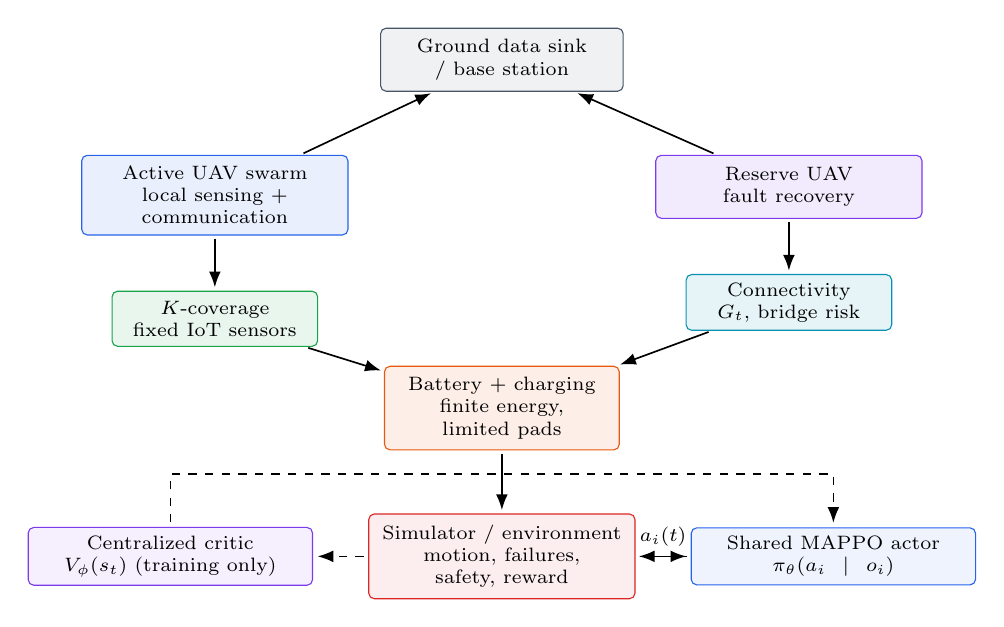
\begin{tikzpicture}[
node distance=6mm and 8mm,
box/.style={draw,rounded corners=2pt,align=center,font=\scriptsize,minimum height=8mm,inner sep=4pt},
small/.style={draw,rounded corners=2pt,align=center,font=\scriptsize,minimum height=7mm,inner sep=3pt},
arr/.style={-{Latex[length=2mm]},semithick,shorten >=1.2pt,shorten <=1.2pt},
darr/.style={-{Latex[length=2mm]},semithick,dashed,shorten >=1.6pt,shorten <=1.6pt}
]
\node[box,fill=uavgray!8,draw=uavgray,text width=28mm] (sink) {Ground data sink\\/ base station};
\node[box,fill=uavblue!10,draw=uavblue,text width=31mm,below left=8mm and 4mm of sink] (swarm) {Active UAV swarm\\local sensing + communication};
\node[box,fill=uavpurple!10,draw=uavpurple,text width=31mm,below right=8mm and 4mm of sink] (reserve) {Reserve UAV\\fault recovery};
\node[small,fill=uavgreen!10,draw=uavgreen,text width=24mm,below=7mm of swarm] (cov) {$K$-coverage\\fixed IoT sensors};
\node[small,fill=uavcyan!10,draw=uavcyan,text width=24mm,below=7mm of reserve] (conn) {Connectivity\\$G_t$, bridge risk};
\node[box,fill=uavorange!10,draw=uavorange,text width=27mm,below=7mm of $(cov)!0.5!(conn)$] (energy) {Battery + charging\\finite energy, limited pads};
\node[box,fill=uavred!8,draw=uavred,text width=31mm,below=8mm of energy] (env) {Simulator / environment\\motion, failures, safety, reward};
\node[small,fill=uavblue!8,draw=uavblue,text width=34mm,right=7mm of env] (actor) {Shared MAPPO actor\\$\pi_\theta(a_i\mid o_i)$};
\node[small,fill=uavpurple!8,draw=uavpurple,text width=34mm,left=7mm of env] (critic) {Centralized critic\\$V_\phi(s_t)$ (training only)};
\draw[arr] (swarm) -- (sink);
\draw[arr] (reserve) -- (sink);
\draw[arr] (swarm) -- (cov);
\draw[arr] (reserve) -- (conn);
\draw[arr] (cov) -- (energy);
\draw[arr] (conn) -- (energy);
\draw[arr] (energy) -- (env);
\draw[darr] (env) -- (actor);
\draw[darr] (env) -- (critic);
\draw[arr] (actor.west) -- node[above,font=\scriptsize] {$a_i(t)$} (env.east);
\coordinate (cfb) at ($(env.north)+(0,5mm)$);
\draw[darr] (critic.north) -- (critic.north |- cfb)
      -- (actor.north |- cfb) -- (actor.north);
\end{tikzpicture}%
}
\caption{Color-coded system architecture. Active UAVs provide sensor coverage and maintain a range-limited communication graph. The reserve UAV supports post-failure recovery. The shared MAPPO actor is deployed locally, while the centralized critic is used only during training.}
\label{fig:arch}
\end{figure}

For tractability, the UAVs fly at a common nominal altitude $z_0$, so the decision process operates in the horizontal plane while the altitude remains part of the physical state. Let $\mathbf p_i(t)=[x_i(t),y_i(t)]^\mathsf{T}$ denote the horizontal position of UAV $i$ and $\mathbf q_d=[x_d,y_d]^\mathsf{T}$ the position of sensor $d$.

\subsection{Dec-POMDP Formulation}
The cooperative control problem is represented as
\begin{equation}
\mathcal G=\langle N,\mathcal S,\{\mathcal A_i\},\{\mathcal O_i\},\mathcal T, R,\gamma\rangle,
\label{eq:decpomdp}
\end{equation}
where $\mathcal S$ is the global state space, $\mathcal A_i$ is the action space of UAV $i$, $\mathcal O_i$ is its local observation space, $\mathcal T$ is the transition model, $R$ is the shared reward, and $\gamma\in(0,1)$ is the discount factor. The training objective is
\begin{equation}
\max_{\pi}\;\mathbb E_{\pi}\left[\sum_{t=0}^{T-1}\gamma^t R_t\right].
\label{eq:objective}
\end{equation}

\subsection{Global State}
The state available to the centralized critic during training is
\begin{equation}
\mathbf s_t=\left\{(\mathbf p_i,\mathbf v_i,b_i,m_i,F_i)_{i=1}^{N},(\mathbf q_d)_{d=1}^{M},\mathbf Q_t\right\},
\label{eq:state}
\end{equation}
where $\mathcal{V}_t^{\mathrm{act}}=\{\,i\in\{1,\dots,N\}:F_i(t)=0\,\}$ is the set of active UAVs, from which any UAV with $F_i(t)=1$ is removed in all coverage, connectivity and energy sums. $\mathbf v_i$ is velocity, $b_i\in[0,1]$ is normalized battery level, $m_i\in\{\mathrm{serve},\mathrm{return},\mathrm{charge}\}$ is operating mode, $F_i\in\{0,1\}$ is the failure indicator, and $\mathbf Q_t\in\{0,1\}^{S}$ records charging-pad occupancy. A failed UAV is removed from the active set used in coverage and connectivity calculations.

The critic sees the joint state, so it is a function of the coverage deficit and can represent it; but the state does not carry the per-sensor coverage counts $n_d(t)$ directly, so the critic has to infer the deficit from the geometry of the UAV and sensor positions. That distinction matters for the credit assignment: a critic that could read $n_d(t)$ would face a different problem from one that must reconstruct it, and the difference is not visible in the reward. The same asymmetry appears on the actor's side, and it is the reason the ego-centric summary of the deficit is part of the observation model.

\subsection{Local Observation}
At deployment, UAV $i$ uses only locally available information:
\begin{equation}
\begin{split}
\mathbf o_i(t)=\bigl[&\mathbf p_i,\mathbf v_i,b_i,\mathcal N_i,C_i^{\mathrm{local}},\rho_i,\tau_i^{\mathrm{return}},\\
&E_i^{\mathrm{pad}},\{\hat{\mathbf u}_{i,j},d_{i,j}\}_{j=1}^{k},\mathbf r_i\bigr].
\end{split}
\label{eq:obs}
\end{equation}
Here $\mathcal N_i$ is the set of nearby UAVs, $C_i^{\mathrm{local}}$ is the number of nearby sensors currently covered, $\rho_i$ is a locally computed bridge-risk estimate, $\tau_i^{\mathrm{return}}$ is the estimated time until the return threshold is reached, and $E_i^{\mathrm{pad}}$ is the estimated energy needed to reach a feasible charging pad.  The final block is the ego-centric deficit summary: for the $k=3$ sensors nearest to $i$ whose coverage is below the required level ($n_d(t)<K$), the agent receives the unit bearing $\hat{\mathbf u}_{i,j}$ and the normalised distance $d_{i,j}$; $\mathbf r_i$ is a repulsion vector away from the centroid of the UAVs in communication range, which keeps a shared policy from collapsing all agents onto the same deficit.  Both are computable from local information under the communication model of Section~\ref{sec:radio}, so the observation is decentralised and has fixed size independent of $M$.

The evaluated observation (68 dimensions) combines the base proprioceptive block (position, velocity, battery, mode, neighbourhood features), a $4\times4$ broadcast deficit map, a one-hot agent identity, a pad-bearing block, and the ego-centric block: unit bearings and normalised distances to the $k=3$ nearest under-covered sensors plus a neighbour-repulsion vector (Eq.~\eqref{eq:obs}).  The ego-centric block is the only term that aligns the observation with the cardinal action space; the value-of-information row of Table~\ref{tab:knobs} prices exact global state against the ego summary.  A one-hot identity of length $N$ and the $G\times G$ deficit grid are retained from the base model and are part of the evaluated configuration.

Unlike the idealized global articulation-point indicator sometimes used in analysis, $\rho_i$ is intended to be computable during execution from neighborhood exchange. The simulator may additionally compute the exact articulation-point indicator for evaluation and for the centralized critic. This distinction avoids assuming that an individual UAV can magically obtain the complete global topology. Table~\ref{tab:obs} lists the observation variables each agent actually receives, and which of them are for the actor and which for the critic.

\begin{table}[t]
\caption{Local observation variables available to each deployed UAV.}
\label{tab:obs}
\centering
\scriptsize
\renewcommand{\arraystretch}{1.06}
\begin{tabularx}{\columnwidth}{@{}L{1.3cm}L{1.7cm}Y@{}}
\toprule
Feature & Symbol & Meaning at decision time \\
\midrule
Position & $\mathbf p_i$ & Own horizontal location; altitude is fixed for the primary study. \\
Velocity & $\mathbf v_i$ & Current velocity for motion-limit awareness. \\
Battery & $b_i$ & Normalized remaining energy. \\
Neighbors & $\mathcal N_i$ & UAVs detected within $R_{\mathrm{comm}}$. \\
Coverage & $C_i^{\mathrm{local}}$ & Nearby sensors currently within coverage radius. \\
Bridge risk & $\rho_i$ & Local estimate of topology criticality. \\
Return urgency & $\tau_i^{\mathrm{return}}$ & Estimated time until the return-energy threshold. \\
Pad energy & $E_i^{\mathrm{pad}}$ & Estimated energy to the nearest feasible charging pad. \\
Deficit bearings & $\{\hat{\mathbf u}_{i,j},d_{i,j}\}_{j=1}^{k}$ & Unit bearing and normalised distance to the $k=3$ nearest under-covered sensors; decentralised, fixed size. \\
Repulsion & $\mathbf r_i$ & Away from the centroid of nearby UAVs; prevents the swarm from collapsing onto one deficit. \\
\bottomrule
\end{tabularx}
\end{table}

\subsection{Discrete Action Space and Motion}
Each active UAV selects one of six actions:
\begin{equation}
\mathcal A_i=\{\mathrm{Hover},+x,-x,+y,-y,\mathrm{Charge}\},\qquad |\mathcal A_i|=6.
\label{eq:actions}
\end{equation}
For movement actions,
\begin{equation}
\mathbf p_i(t+1)=\Pi_{\Omega}\left(\mathbf p_i(t)+\mathbf v_i(t)\Delta t\right),
\qquad \|\mathbf v_i(t)\|\le v_{\max},
\label{eq:motion}
\end{equation}

\begin{table}[t]
\caption{Discrete action semantics used by the MAPPO actor.}
\label{tab:actions}
\centering
\scriptsize
\renewcommand{\arraystretch}{1.05}
\begin{tabularx}{\columnwidth}{@{}L{1.35cm}Y@{}}
\toprule
Action & Effect \\
\midrule
Hover & Remain at the current position and continue serving covered sensors. \\
$+x$ / $-x$ & Move by one control step along the horizontal $x$ direction. \\
$+y$ / $-y$ & Move by one control step along the horizontal $y$ direction. \\
Charge & Request charging when inside a pad service region; pad selection is handled by the scheduler. \\
\bottomrule
\end{tabularx}
\end{table}
where $\Pi_{\Omega}$ projects into the permitted airspace. A charge request is feasible only when the UAV is inside a station neighborhood of a free pad. Table~\ref{tab:actions} gives the effect of each of the six actions. The RL layer does not select a pad as part of its action; pad choice is handled by the arbitration layer in Section~\ref{sec:charging}.

\subsection{Persistent \texorpdfstring{$K$}{K}-Coverage}
\label{sec:coverage}
A UAV covers sensor $d$ in slot $t$ when
\begin{equation}
x_{id}(t)=\mathbb 1\!\left[\|\mathbf p_i(t)-\mathbf q_d\|_2\le R_{\mathrm{cov}}\right].
\label{eq:xid}
\end{equation}
The number of active UAVs covering sensor $d$ is
\begin{equation}
n_d(t)=\sum_{i\in\mathcal V_t^{\mathrm{act}}}x_{id}(t),
\label{eq:nd}
\end{equation}
and the instantaneous normalized coverage score is
\begin{equation}
C_t=\frac{1}{M}\sum_{d=1}^{M}\min\left(\frac{n_d(t)}{K},1\right).
\label{eq:Ct}
\end{equation}
The instantaneous under-coverage rate is
\begin{equation}
U_t=\frac{1}{M}\sum_{d=1}^{M}\mathbb 1[n_d(t)<K].
\label{eq:Ut}
\end{equation}
The primary service condition is $n_d(t)\ge K$ for all $d$ whenever the geometry and available fleet make it feasible. The condition \eqref{eq:xid} is the geometric half of it: a UAV counts towards a sensor's coverage only if the link to that sensor is also serviceable, which the radio model of Section~\ref{sec:radio} supplies, and the simulator applies the two together. The two requirements, coverage and connectivity, are not independent, and Figure~\ref{fig:coupling} shows the three dimensions in which they are coupled: the same UAV flies to cover a sensor and to keep the communication graph connected, and the two requirements compete for the same flight and energy budget.

\medskip
\noindent\textbf{Feasibility.} Persistent $K$-coverage is achievable only when the sensing radius is large enough for the available fleet. Comparing the area available for coverage with the area required gives a necessary condition: $N$ disks of radius $R_{\mathrm{cov}}$ supply $N\pi R_{\mathrm{cov}}^{2}$, while $K$-coverage of a region of area $A$ requires $KA$. Hence $R_{\mathrm{cov}} \ge \sqrt{KA/(\pi N)}$. Accounting for the $\delta = \pi/(2\sqrt{3}) \approx 0.907$ packing density of congruent disks gives the stricter form $R_{\mathrm{cov}} \ge \sqrt{KA/(\delta\pi N)}$. Substituting the parameters of Table~\ref{tab:parameters} ($A = 6400$ m$^2$, $M = 20$, $N = 5$, $K = 2$) yields $R_{\mathrm{cov}} \ge 28.5$ m by area counting and $30.0$ m after the packing correction, both satisfied by the chosen $R_{\mathrm{cov}} = 35$ m. The surplus ratio $\sigma = N\pi R_{\mathrm{cov}}^{2}/(KA) = 1.50$ that follows is the conventional area-surplus test: it is the criterion by which much of the prior work declares a configuration feasible, and it is satisfied here by a margin of one half. Section~\ref{sec:feasibility} shows that being satisfied certifies nothing, and the reason is worth stating here rather than there, because the two criteria are easy to confuse. $\sigma$ compares an area to an area, while $K$-covering a bounded region is a covering problem: the four corner points of the square are more than $2R_{\mathrm{cov}}$ apart, so no disc can serve two of them, and the packing bound of the next section then requires $N \ge 4K = 8$ for this configuration, the same configuration that $\sigma$ passes. The bound above is necessary rather than sufficient in a second way as well, since it ignores coverage-disk overlap and the discreteness of the sensor layout; scenario S6 of Table~\ref{tab:scenarios} therefore sweeps $R_{\mathrm{cov}}$ directly to characterize the transition.

\begin{figure}[t]
\centering
% 3D schematic: oblique axonometric. UAVs fly at z_0 above the sensor plane.
% No \resizebox here: it would scale line widths and dash patterns too.
% The unit vectors below give the natural size (about 73 x 51 mm), which fits
% the 88.9 mm IEEE column width at true line widths and font sizes.
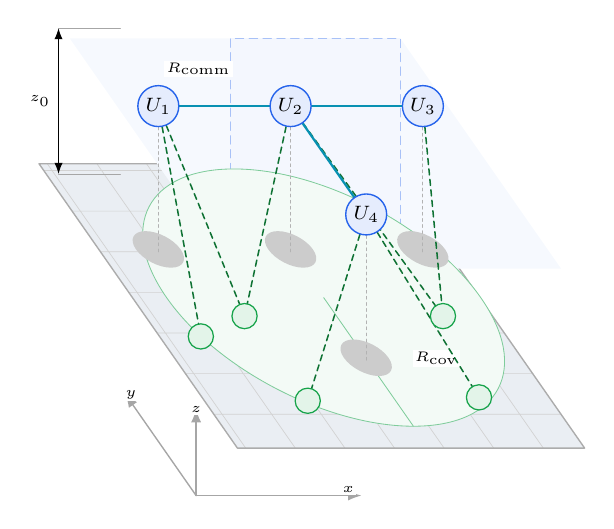
\begin{tikzpicture}[
pt/.style={circle,draw=uavblue,fill=uavblue!12,line width=0.5pt,
           minimum size=5.2mm,inner sep=0pt,font=\scriptsize},
sn/.style={circle,draw=uavgreen,fill=uavgreen!12,line width=0.45pt,
           minimum size=3.2mm,inner sep=0pt},
link/.style={draw=uavcyan,line width=0.8pt},
covlink/.style={draw=uavgreen!70!black,line width=0.55pt,
                dash pattern=on 2.2pt off 1.6pt},
drop/.style={draw=gray!60,line width=0.35pt,dash pattern=on 1pt off 1.2pt},
foot/.style={draw=uavgreen!55,line width=0.3pt,fill=uavgreen!5},
uavpl/.style={draw=uavblue!40,line width=0.4pt,
              dash pattern=on 3pt off 2pt,fill=uavblue!5},
guide/.style={draw=gray!70,line width=0.25pt},
axis/.style={-{Latex[length=1.7mm]},line width=0.5pt,draw=gray!70},
shadow/.style={fill=gray!40,draw=none},
ann/.style={font=\tiny,align=center,fill=white,inner sep=0.8pt},
x={(1.05cm,0cm)}, y={(-0.6cm,0.86cm)}, z={(0cm,1cm)},
line cap=round, line join=round
]
%  ground plane (fixed IoT sensors live on it) 
\begin{scope}[canvas is xy plane at z=0]
  \path[fill=gndgray] (-0.7,-2.9) rectangle (3.5,1.3);
  \draw[step=0.6,gray!35,line width=0.25pt] (-0.7,-2.9) grid (3.5,1.3);
  \draw[gray!65,line width=0.5pt] (-0.7,-2.9) rectangle (3.5,1.3);
\end{scope}
%  UAV operating plane at altitude z_0 (translucent, in front) 
\begin{scope}[canvas is xy plane at z=1.85]
  \path[fill=uavblue!4] (-0.5,-2.4) rectangle (3.5,1.0);
\end{scope}
\draw[uavpl] (-0.5,-2.4,1.85) rectangle (3.5,1.0,1.85);
%  horizontal coverage footprint, drawn on the ground 
\begin{scope}[canvas is xy plane at z=0.02]
  \draw[foot] (1.6,-0.7) circle[radius=1.9];
  \draw[foot] (1.6,-0.7) -- (1.6,-2.6);
  \node[ann] at (2.45,-1.6) {$R_{\mathrm{cov}}$};
\end{scope}
%  ground shadows + vertical drop lines (depth cues) 
\foreach \cx/\cy in {0/0,1.6/0,3.2/0,1.6/-1.6}{
  \begin{scope}[canvas is xy plane at z=0.03]
    \fill[shadow] (\cx,\cy) circle[radius=0.27];
  \end{scope}
  \draw[drop] (\cx,\cy,0) -- (\cx,\cy,1.85);
}
%  coverage links 
\draw[covlink] (0,0,1.85)      -- (-0.2,-1.25,0);
\draw[covlink] (0,0,1.85)      -- (0.5,-0.95,0);
\draw[covlink] (1.6,0,1.85)    -- (0.5,-0.95,0);
\draw[covlink] (1.6,0,1.85)    -- (2.9,-0.95,0);
\draw[covlink] (3.2,0,1.85)    -- (2.9,-0.95,0);
\draw[covlink] (1.6,-1.6,1.85) -- (0.55,-2.2,0);
\draw[covlink] (1.6,-1.6,1.85) -- (2.65,-2.15,0);
%  sensors on the plane 
\foreach \cx/\cy in {-0.2/-1.25,0.5/-0.95,2.9/-0.95,0.55/-2.2,2.65/-2.15}
  \node[sn] at (\cx,\cy,0) {};
%  inter-UAV communication (all at equal altitude) 
\draw[link] (0,0,1.85) -- (1.6,0,1.85) -- (3.2,0,1.85);
\draw[link] (1.6,0,1.85) -- (1.6,-1.6,1.85);
\node[ann] at (0.8,0.55,1.85) {$R_{\mathrm{comm}}$};
%  UAVs (drawn last so they sit on top) 
\node[pt] at (0,0,1.85)      {$U_1$};
\node[pt] at (1.6,0,1.85)    {$U_2$};
\node[pt] at (3.2,0,1.85)    {$U_3$};
\node[pt] at (1.6,-1.6,1.85) {$U_4$};
%  altitude dimension z_0 
\draw[guide] (-0.55,1.15,0)    -- (0.2,1.15,0);
\draw[guide] (-0.55,1.15,1.85) -- (0.2,1.15,1.85);
\draw[{Latex[length=1.4mm]}-{Latex[length=1.4mm]},line width=0.4pt]
      (-0.55,1.15,0) -- (-0.55,1.15,1.85)
      node[ann,midway,left=2pt] {$z_0$};
%  projected x/y/z triad: unambiguous 3D frame 
\draw[axis] (-1.6,-3.6,0) -- (0.4,-3.6,0)   node[ann,pos=0.92,above] {$x$};
\draw[axis] (-1.6,-3.6,0) -- (-1.6,-2.1,0)   node[ann,pos=0.92,above] {$y$};
\draw[axis] (-1.6,-3.6,0) -- (-1.6,-3.6,1.1) node[ann,pos=0.92,above] {$z$};
\end{tikzpicture}
\caption{Coupling between coverage and connectivity in three dimensions. The shaded grid is the fixed sensor plane at $z=0$, and the translucent blue sheet is the UAV operating plane at the common nominal altitude $z_0$; the projected $x/y/z$ triad, the ground shadows and the dashed vertical drop lines fix the perspective. The green disc on the ground is the horizontal coverage footprint $R_{\mathrm{cov}}$ joined to the UAVs by dashed coverage links, whereas the cyan edges lying inside the UAV plane are inter-UAV communication links of range $R_{\mathrm{comm}}$. Removing a topologically critical UAV can reduce both service redundancy and network connectivity.}
\label{fig:coupling}
\end{figure}

\subsection{Feasibility Certificate for \texorpdfstring{$K$}{K}-Coverage}
\label{sec:feasibility}

Before any policy is trained, the configuration must be shown to admit a
feasible solution.  Two different requirements have to be separated here,
because they have different certificates: the requirement that every point
of the operational region $\Omega$ is $K$-covered, and the requirement that
every one of the $M$ sensors is $K$-covered.  The second is what the
experiments measure, and the distinction is not academic: the corner
argument that settles the first does not settle the second.

\emph{The packing lemma.} Let $A$ be the set of points to be $K$-covered and
define the \emph{packing number}
\begin{equation}
P(A,R)=\max\bigl\{\,|X|:\ X\subseteq A,\ \|x-x'\|>2R\ \ \forall x\neq x'\,\bigr\}.
\label{eq:packing}
\end{equation}
Then $A$ cannot be $K$-covered by fewer than $K\,P(A,R)$ discs of radius
$R$.  The proof is one line: a disc of radius $R$ contains at most one
point of $X$, because two such points would be within $2R$; so the discs
that serve the $K$ coverings of each point of $X$ are pairwise disjoint
across distinct points, and each point consumes $K$ of them.  This is a
first-principles covering argument, no disc covers two corners because
they are more than $2R_{\mathrm{cov}}$ apart, and each corner must be
covered $K$ times, and it is the only form of it that applies to an
arbitrary point set.

\emph{Region bound.} For $A=\Omega$ and the four corners of the square,
the four corners of the $80\times80$\,m square are $80$\,m apart along a side and $80\sqrt2\approx113$\,m apart on the diagonal, both larger than $2R_{\mathrm{cov}}=70$\,m, so the four corner discs are pairwise disjoint and $P(\Omega,R_{\mathrm{cov}})=4$: partition $\Omega$ into four $40\times40$ sub-squares, whose diameter $40\sqrt2=56.6$\,m is below $2R_{\mathrm{cov}}$, so no two packed points share a sub-square, and the four corners attain the bound.  By \eqref{eq:packing}, $K$-covering the region therefore requires
\begin{equation}
N\ \ge\ 4K\ =\ 8 .
\label{eq:regionbound}
\end{equation}
The report's original $N=5$, $K=2$, $R_{\mathrm{cov}}=35$\,m configuration
is therefore \emph{provably infeasible} for the region requirement, and
\eqref{eq:regionbound} is \emph{tight} at these parameters: the four points
$\{(20,20),(60,20),(20,60),(60,60)\}$ cover the square once, since the
farthest point of a cell from its centre is $40/\sqrt2=28.28$\,m $<35$\,m,
and $K$ layers of those points, each displaced by a distinct vector of
norm at most $35-28.28=6.72$\,m, cover it $K$ times with $4K$ discs.  So
$N=8$ is not merely sufficient for the region; it is exactly sufficient.

\emph{Sensor-set bound, and what the corner certificate does not say.} The
sensors are not at the corners, so \eqref{eq:regionbound} does not transfer
to them.  It would transfer if the sensor set contained four sensors whose
coverage discs were pairwise disjoint, and a sufficient condition for that
is one sensor in each of four corner caps of radius below
$\tokCapR\,\mathrm{m}$: two sensors in adjacent caps are then at least
$80-2r$ apart, and their discs are disjoint while
$80-2r>2R_{\mathrm{cov}}=\tokCapTwoR\,\mathrm{m}$, the adjacent pair
being the binding one (a diagonal pair is $80\sqrt2-2r$ apart).  The
condition is sufficient and not necessary, a packing of four sensors
more than $\tokCapTwoR$ m apart can occur anywhere and not only near the
corners, but a random draw essentially never meets it: a cap of that
radius is $\tokCapPct\%$ of the square, and a uniform draw of $20$ sensors
lands one in each of the four caps with probability $\tokCapP$.  The
applicable bound is \eqref{eq:packing} applied to the realised sensor set.
Measured over $\tokPackSeeds$ random draws
(\texttt{analysis/feasibility.py}), the packing number has mean
$\tokPackMean$ and range $\tokPackMin$--$\tokPackMax$, so the bound is
$N\ge \tokPackNMean$ on average and $N\ge \tokPackNMax$ in the worst
case, and $N=5$ is \emph{excluded} for $\tokPackExcluded$ of the
$\tokPackSeeds$ draws ($\tokPackExclPct\%$).  On the scenes on which the
teleporting oracle was measured it reaches $CK=\tokInfOracle$ at $N=5$, so
the sensor requirement does not obstruct $N=5$ there; what that
measurement does not do is certify feasibility for the remaining draws,
and the correct statement is a probabilistic one, not a certificate.  We state this rather than the
convenient one: the configuration is \emph{provably} infeasible for the
region, and
\emph{probably} infeasible for a minority of sensor draws.

\emph{This configuration is feasible for both requirements.}
$N=8$, $K=2$, $R_{\mathrm{cov}}=35$\,m satisfies \eqref{eq:regionbound}
with equality and the construction above, so every sensor is $K$-covered
for \emph{every} sensor layout, not merely for the ones that were drawn.
The teleporting oracle of Section~\ref{sec:feasibility} confirms it,
reaching $CK=1.000$ with a connected placement.

\emph{The area-surplus criterion certifies nothing.} The metric
$\sigma=N\pi R_{\mathrm{cov}}^{2}/(K|\Omega|)$ equals $1.503$ at $N=5$ and
exceeds one, and the configuration is nonetheless infeasible for the region.
The reason is that area is a measure condition and covering is a pointwise
one: $N$ discs can be piled over a small patch, satisfying $\sigma>1$ while
most of $\Omega$ is uncovered, and conversely a clustered sensor set can be
covered with $\sigma<1$.  In particular $\sigma\ge1$ is \emph{necessary}
for $K$-covering the region and is \emph{not even necessary} for
$K$-covering a sensor set, and it is never sufficient: at $N=7$, $K=2$ it is
$2.10$ and the region bound \eqref{eq:regionbound} still excludes the
configuration.  A feasibility certificate has to be a covering argument.

\emph{What the degenerate metric does, exactly.} Let $\mathcal{F}$ be the
set of configurations in which every sensor is $K$-covered and the
communication graph is connected.  The service-continuity metric of
Table~\ref{tab:metrics} satisfies
\begin{equation}
\mathcal{F}=\varnothing \quad\Longrightarrow\quad SC(\pi)=0\ \text{for every policy }\pi,
\label{eq:scdegenerate}
\end{equation}
because $SC(\pi)>0$ requires the trajectory to visit $\mathcal{F}$ at some
instant.  The converse does not hold: a poor policy on a feasible instance
may also score zero, so observing $SC(\pi)=0$ does not prove infeasibility.
The statement is therefore about the best achievable value
$\max_\pi SC(\pi)$ and not about the value any particular policy realises:
a poor policy on a perfectly feasible instance also scores $SC=0$.  When
$\mathcal{F}=\varnothing$ the metric is uninformative, and the
time-averaged coverage deficit of the same table is not, which is the
point of reporting it alongside.

\emph{Feasible deployments:} $N=8$, $K=2$, $R_{\mathrm{cov}}=35$\,m
(provably feasible for both requirements, and tight against the region
bound) or $N=5$, $K=2$, $R_{\mathrm{cov}}=45$\,m, for which four discs at
the midpoints of the region's sides and one at its centre cover every point
of the region at least twice, the worst second-nearest distance being
$\tokAltNfiveR$\,m against the $45$\,m offered. All trained results in this
report use the reported eight-UAV deployment.

\emph{Achievability ceiling.} A teleporting placement oracle
(\texttt{analysis/feasibility.py}) places the $N$ UAVs anywhere, at no
motion cost and ignoring energy, and upper-bounds the coverage fraction
$C_K$ of any policy, because the per-step coverage fraction of any
trajectory is bounded by the best static placement.  It therefore separates
``the policy is weak'' from ``the task is infeasible'', and it is the
ceiling against which the reported coverage is read.  Two limits on the
claim are worth stating.  The oracle is an upper bound on $C_K$ and \emph{not}
on the service-continuity metric, which additionally requires the
requirement to hold at every instant of a kinematically constrained
trajectory; and it does not certify that a feasible trajectory achieving the
certified coverage exists.  That last point is checked rather than
assumed: the construction of \eqref{eq:regionbound} is admissible under
the simulator's own safety filter, its communication graph is connected,
it has no articulation point, and its eccentricity is $3$, within the
$H$-hop rule, so the certified configuration is reachable by a policy
and the ceiling is comparable with what a policy can achieve.  The
normalisation by the oracle is, at this configuration, the identity, since
the ceiling is $1.000$ for every sensor layout; its information is that the
task is coverable at all with $N=8$. Since the construction is itself
admissible under the safety filter, the \emph{constrained} ceiling is
the same $1.000$: the constraint removes no headroom, so there is no
second ceiling to compute, and the normalisation by the oracle is
meaningful at this configuration rather than vacuous.  At this configuration the value is
$C_K=1.000$ and it is attained for \emph{every} sensor layout, because the
construction of \eqref{eq:regionbound} covers the whole region, so the
ceiling is deterministic rather than a random variable over layouts.

\emph{Non-degenerate metrics.} The service-continuity metric
``fraction of time all sensors are $K$-covered \emph{and} the graph is
connected'' is identically zero for every policy when $\mathcal{F}$ is
empty, by \eqref{eq:scdegenerate}.  It is retained for comparison, and
reported alongside two quantities that are not.  The first is the
time-averaged coverage deficit $\frac1T\sum_t(1-\overline{\mathrm{CK}}_t)$,
which is graded: it gives partial credit for a near miss, where the binary
flag gives none, and it is the better-behaved quantity as a training
signal.  We note that it is, exactly, the complement of the coverage
fraction $C_K$, so it is a change of convention rather than an independent
measurement, and that it is blind to the connectivity half of the
requirement.  The second is the maximum refresh time, the longest run of
consecutive steps with any under-covered sensor, which is not a function of
$C_K$: a controller can hold a high average coverage while leaving one
sensor dark for a long time, and the refresh time is what detects that.  It
is the maximum refresh time, rather than the deficit, that carries the
information the binary flag cannot.

\subsection{Energy-Flow Feasibility}
\label{sec:energyflow}

The spatial certificate of Section~\ref{sec:feasibility} answers ``are there
enough UAVs to cover the region''.  The conservation reasoning below is
not new in substance: fleet-sizing laws express it in time units for
homogeneous recharge (Arribas et al.~\cite{arribas2023}; Ramesh and
Thomas~\cite{ramesh2026}), and energy-aware LP scheduling has been used
for K-coverage with charging platforms (Song et al.~\cite{song2024}).
The contribution here is the power-flow form used as a certificate, the
finite-horizon bound, and the explicit no-fly-while-charging constraint,
which together make the ceiling computable before any learning and
non-vacuous at the reported configuration.  It does not answer the question a
reviewer will ask next: ``can the fleet stay airborne long enough for the
coverage to be \emph{persistent} rather than a one-battery sprint''.  The
answer is obtained from the same geometry, now with the battery and the
charging pads in the loop.

Let $P_{\mathrm{air}} = P_{\mathrm{hover}} + P_{\mathrm{elec}} + P_{\mathrm{tx}}$
be the power drawn by an airborne UAV and let $P_{\mathrm{pad}}^{\mathrm{net}}$
be the net charging power of one pad.  At the reported parameters
$P_{\mathrm{air}} = 55.1\,\mathrm{W}$ and $P_{\mathrm{pad}}^{\mathrm{net}}
= 24.9\,\mathrm{W}$ (a $30\,\mathrm{W}$ gross charge rate minus the
$5.1\,\mathrm{W}$ avionics draw of a charging UAV).

\paragraph{Steady-state bound.}  In the long run the fleet can keep airborne
at most
\[
n_{\mathrm{air}}^{\mathrm{ss}}
= \frac{S\,P_{\mathrm{pad}}^{\mathrm{net}}}{P_{\mathrm{air}}}
\]
UAVs, where $S$ is the number of pads.  With $S=2$ this is
$0.90$ UAVs against the $N_{\min}=4K=8$ required by the spatial
certificate, a deficit of $7.1$ UAVs.  The persistent coverage ceiling is
therefore
\[
C_K^{\mathrm{ss}} = \min\!\left(1,\;\frac{n_{\mathrm{air}}^{\mathrm{ss}}}{N_{\min}}\right)
= 0.113 .
\]
\emph{The reported configuration is not persistently feasible:} no policy,
however clever, can sustain $K$-coverage indefinitely at it, because the
pads cannot replace the energy the fleet spends.  This is the energy
analogue of the spatial infeasibility of $N=5$: the framework now says so
about energy as well as space, which is the point of having a certificate.

\paragraph{Finite-horizon bound.}  Over a mission of $T$ seconds the
airborne UAV-seconds are capped by
\[
\frac{E_{\mathrm{stored}} + S\,P_{\mathrm{pad}}^{\mathrm{net}}\,T}{P_{\mathrm{air}}},
\qquad
E_{\mathrm{stored}} = N\,E_0 .
\]
At the reported episode length $T=400\,\mathrm{s}$ this gives a ceiling of
$1.000$: the episode is feasible, but only by drawing down the initial
packs, and the energy constraint binds (the Reactive heuristic records
$\tokReactRet$ return-to-charge transitions per episode).  At the
$10\,000$-step target ($T=2000\,\mathrm{s}$) the ceiling falls to
$0.367$ with full packs and $0.326$ at the mean initial charge of $0.85$,
so a policy evaluated at that horizon could not exceed roughly a third of
full $K$-coverage on energy grounds alone.  The $400\,\mathrm{s}$ result
is therefore a finite-horizon result, and the report says so explicitly.

\paragraph{Energy-aware ceiling (LP).}  A fluid relaxation maximises the
time-averaged airborne fleet subject to per-UAV energy, pad throughput, and
no-fly-while-charging, and gives the same ceiling as the bound above at
$T=400\,\mathrm{s}$ ($1.000$) and $T=2000\,\mathrm{s}$ ($0.367$).  It is
the energy analogue of the teleporting placement oracle: an upper bound no
online policy can beat, and the quantity against which an energy-aware
controller should be normalised.

\paragraph{What would make it persistent.}  A sweep over hardware parameters
shows that none of the single changes (four pads, $60\,\mathrm{kJ}$ packs,
$0.0004$ charge rate, or $12$ UAVs) reaches feasibility on its own; only
the combination ($N=12$, $S=4$, $B^{\max}=60\,\mathrm{kJ}$,
$0.0004$ charge rate) does, with a steady-state ceiling of $1.000$ and
small slack.  Persistent $K$-coverage at these power levels is a
hardware-budget question before it is a control question, which is exactly
what a certificate is for.

\paragraph{Scope.}  The energy certificate does not replace the spatial one;
it complements it.  A configuration must pass both to be called persistent,
and the reported configuration passes the spatial test and fails the energy
one beyond $400\,\mathrm{s}$.  The coverage numbers in Section~\ref{sec:results}
are therefore finite-horizon numbers, and the framework now says so.
\subsection{Connectivity Model}
The inter-UAV communication graph is
\begin{equation}
G_t=(V_t,E_t),\qquad E_t=\{(i,j):\|\mathbf p_i-\mathbf p_j\|_2\le R_{\mathrm{comm}}\}.
\label{eq:graph}
\end{equation}
The ground data sink is not a vertex of the graph: the connectivity the paper measures is the connectivity of the active-UAV graph, and the sink is assumed to stay within $R_{\mathrm{comm}}$ of at least one UAV, which is an assumption and not a guarantee. For analysis, the exact articulation-point indicator, where $G_t^{-i}$ denotes $G_t$ with vertex $i$ and its incident edges removed, is
\begin{equation}
\kappa_i(t)=\mathbb 1\left[G_t^{-i}\;\text{is disconnected}\right].
\label{eq:articulation}
\end{equation}
The average criticality is
\begin{equation}
\mathrm{Crit}_t=\frac{1}{|V_t^{\mathrm{act}}|}\sum_{i\in V_t^{\mathrm{act}}}\kappa_i(t).
\label{eq:crit}
\end{equation}
The exact graph quantity is used by the simulator for evaluation. The actor receives the local proxy $\rho_i$ rather than the full graph.

\subsection{The Radio Model, and What It Gates}
\label{sec:radio}
The graph of \eqref{eq:graph} and the coverage condition of \eqref{eq:xid} are both geometric, and both are gated by a radio model: a UAV counts towards a sensor's coverage, and two UAVs count as adjacent, only when the link between them carries a usable service rate. The gate is what makes the discs physical rather than notional, and it is stated here because the two conditions above are otherwise read as purely geometric.

The air-to-ground path follows the Al-Hourani model~\cite{alhourani2014}: for a UAV at altitude $z_0$ and a slant range $d_3$ to the ground node, the elevation angle $\theta=\arcsin(z_0/d_3)$ gives the probability of an unobstructed path,
\begin{equation}
P(\mathrm{LoS})=\frac{1}{1+a\,e^{-b(\theta-a)}},\qquad a=9.61,\quad b=0.16,
\label{eq:los}
\end{equation}
and the path loss blends a log-distance law for the clear path with one for the obstructed path,
\begin{equation}
\begin{split}
PL(d)&=P(\mathrm{LoS})\,PL_{\mathrm{LoS}}(d)+\bigl(1-P(\mathrm{LoS})\bigr)\,PL_{\mathrm{NLoS}}(d),\\
PL_{\cdot}(d)&=PL(d_0)+10\,n_{\cdot}\log_{10}\frac{d}{d_0},
\end{split}
\label{eq:pl}
\end{equation}
with $PL(d_0)=20\log_{10}\!\bigl(4\pi d_0 f/c\bigr)$, $d_0=1$~m, $n_{\mathrm{LoS}}=2.0$ and $n_{\mathrm{NLoS}}=3.5$~\cite{3gpp36777}. A shadowing term with a standard deviation of $4$~dB is drawn once per episode, so that shadowing is a property of the scene and not of the step, and the inter-UAV links share one draw per pair because a link is one physical link.

The received power is $P_{\mathrm{tx}}\,10^{-PL/10}$, with $P_{\mathrm{tx}}=0.5$~W at $f=2.4$~GHz, and the noise floor is the thermal noise of a $20$~MHz channel with the receiver's noise figure. The signal-to-noise ratio selects an achievable rate from the IEEE 802.11 OFDM MCS table~\cite{ieee80211}, and a link is \emph{usable} when that rate is at least $6.5$~Mbit/s, the lowest rate in the table. Writing $\mathrm{rate}_{id}$ for the rate that the access link from UAV $i$ to sensor $d$ achieves, and $\mathrm{rate}_{ij}$ for the rate of the inter-UAV link, the two conditions of this paper are therefore the conjunction of a geometric and a radio condition: the coverage count of \eqref{eq:nd} is taken over the summands of \eqref{eq:gate},
\begin{equation}
n_d(t)=\sum_{i\in\mathcal V_t^{\mathrm{act}}}
\underbrace{\mathbb 1\!\left[\|\mathbf p_i-\mathbf q_d\|_2\le R_{\mathrm{cov}}\right]}_{\text{geometry}}
\;\underbrace{\mathbb 1\!\left[\mathrm{rate}_{id}\ge 6.5\right]}_{\text{radio}},
\label{eq:gate}
\end{equation}
and the communication graph of \eqref{eq:graph} carries an edge when $\|\mathbf p_i-\mathbf p_j\|_2\le R_{\mathrm{comm}}$ \emph{and} $\mathrm{rate}_{ij}\ge 6.5$~Mbit/s.
The access link is noise-limited, because the UAVs are assigned orthogonal channels; a co-channel term is implemented and is switched off, since $K$-coverage asks whether $K$ UAVs are \emph{able} to serve a sensor, not whether all $K$ transmit on one resource at the same instant.

Two consequences follow. First, the discs are the geometry and the radio is the budget, and which of the two binds is a measurement rather than an assumption: Section~\ref{sec:validation} measures the link margin at the two operating radii and finds it wide, so the feasibility certificate of Section~\ref{sec:feasibility} and not the radio is what constrains the fleet. Second, because the gate is in the model, the coverage reported here is coverage of \emph{serviceable} links and not of discs.

\subsection{Battery Model}
Let $B_i^{\max}$ be the battery capacity in joules and $E_i(t)=b_i(t)B_i^{\max}$ the remaining energy. The slot energy update is
\begin{equation}
E_i(t+1)=\mathrm{clip}\!\left(E_i(t)-P_i(t)\Delta t+P_{\mathrm{ch},i}(t)\Delta t,\;0,\;B_i^{\max}\right),
\label{eq:battery}
\end{equation}
where the action-dependent consumption is
\begin{equation}
\begin{split}
P_i(t)={}&P_{\mathrm{hover}}\,\mathbb 1[a_i=\mathrm{Hover}]\\
&+P_{\mathrm{move}}\,\mathbb 1[a_i\in\{+x,-x,+y,-y\}]+P_{\mathrm{comm}}.
\end{split}
\label{eq:power}
\end{equation}
The charge power is zero unless the UAV is physically docked and granted service at a pad. A return threshold is defined by
\begin{equation}
E_i^{\mathrm{req}}(t)=E_i^{\mathrm{pad}}(t)+E_i^{\mathrm{rejoin}}(t)+E^{\mathrm{reserve}},
\label{eq:ereq}
\end{equation}
and a return is mandatory when $E_i(t)\le E_i^{\mathrm{req}}(t)$.

Two properties of this model are easy to state and easy to implement incorrectly, and both are pinned by tests. First, the return is a \emph{physical} transition and not a decision available to the policy: the simulator makes it, so that the reward, the metrics and the charging arbitration can all see it. If the simulator does not make it, then a learned policy has no way to express the return at all, the arbitration is never entered, and the reserve mechanism has nothing to recover, the three mechanisms this paper proposes are then present in the model and absent from the experiment. Second, a UAV that is docked and charging has its rotors idle and draws only the avionics and communications baseline; if it is billed the hover power, the pack loses more energy to the rotors than the pad puts back, no UAV can ever recover, and the charging coordination is unusable. A UAV whose pack empties away from a pad is out of service: it can no longer fly, and it must not continue to count towards coverage or towards the connectivity graph. Figure~\ref{fig:statemachine} shows the battery and failure state machine: the transitions between flying, returning to charge, charging and failing, and the point at which the reserve UAV takes over.

\begin{figure}[t]
\centering
\resizebox{\columnwidth}{!}{%
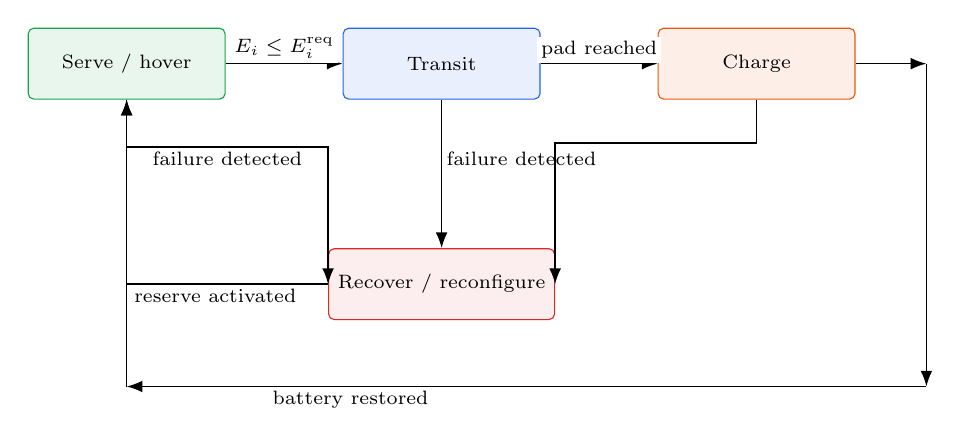
\begin{tikzpicture}[
state/.style={draw,rounded corners=2pt,minimum width=25mm,minimum height=9mm,align=center,font=\scriptsize},
arr/.style={-{Latex[length=2mm]},semithick},
lab/.style={font=\scriptsize,fill=white,inner sep=1.5pt}
]
\node[state,fill=uavgreen!10,draw=uavgreen]  (serve)   at (0,0)     {Serve / hover};
\node[state,fill=uavblue!10,draw=uavblue]    (transit) at (4.0,0)   {Transit};
\node[state,fill=uavorange!10,draw=uavorange] (charge) at (8.0,0)   {Charge};
\node[state,fill=uavred!8,draw=uavred]       (recover) at (4.0,-2.8) {Recover / reconfigure};
\draw[arr] (serve)  -- node[lab,above] {$E_i\le E_i^{\mathrm{req}}$} (transit);
\draw[arr] (serve.south) -- ++(0,-0.6) -| node[lab,below,pos=0.25] {failure detected} (recover.west);
\draw[arr] (transit) -- node[lab,above] {pad reached} (charge);
\coordinate (rt) at ($(charge.east)+(0.9,0)$);
\coordinate (rb) at ($(rt)+(0,-4.1)$);
\draw[arr] (charge.east) -- (rt);
\draw[arr] (rt) -- (rb);
\draw[arr] (rb) -- node[lab,below,pos=0.72] {battery restored} (0,-4.1);
\draw[arr] (0,-4.1) -- (serve.south);
\draw[arr] (transit.south) -- node[lab,right,pos=0.40] {failure detected} (recover.north);
\draw[arr] (charge.south) -- ++(0,-0.55) -| (recover.east);
\draw[arr] (recover.west) -| node[lab,below,pos=0.28] {reserve activated} (serve.south);
\end{tikzpicture}%
}
\caption{Battery and failure state machine. Energy urgency triggers a return-to-charge transition; a detected failure transfers the mission to a recovery phase in which the reserve UAV can be activated when feasible.}
\label{fig:statemachine}
\end{figure}

\subsection{Charging Coordination}
\label{sec:charging}
Charging is a scarce resource. Let $y_{is}\in\{0,1\}$ denote whether UAV $i$ is assigned to pad $s$. For a charge request, define a local assignment cost
\begin{equation}
c_{is}=\alpha\tilde d_{is}+\beta\tilde q_s+\mu\tilde u_i,
\label{eq:chargingcost}
\end{equation}
where $\tilde d_{is}$ is normalized distance, $\tilde q_s$ is normalized queue length, and $\tilde u_i$ is normalized battery urgency. The arbitration layer solves
\begin{equation}
\begin{aligned}
\min_{\mathbf y}\quad &\sum_i\sum_s c_{is}y_{is}\\
\mathrm{s.t.}\quad &\sum_s y_{is}\le1,\ \forall i,\\
&\sum_i y_{is}\le1,\ \forall s,\\
&y_{is}\in\{0,1\}.
\end{aligned}
\label{eq:charging}
\end{equation}
Because only charge requests are handled, this is a small scheduling problem rather than a centralized trajectory controller. A Hungarian-style assignment implementation is sufficient for the expected fleet size.

\subsection{Safety Constraints}
\label{sec:safety_model}
The environment enforces
\begin{equation}
\begin{split}
&\|\mathbf v_i(t)\|\le v_{\max},\qquad \mathbf p_i(t)\in\Omega,\\
&\|\mathbf p_i(t)-\mathbf p_j(t)\|\ge d_{\mathrm{safe}},\ \forall i\ne j.
\end{split}
\label{eq:safety}
\end{equation}
An action is masked if it violates a locally predictable hard constraint such as workspace bounds, speed, minimum separation, or invalid charging. The energy rule deserves a sentence of its own, because a weak version of it is a mechanism rather than a detail: a UAV that may depart with a flat battery will fly until its pack is empty, and an exhausted UAV is removed from the active set, taking its share of the coverage and of the communication graph with it. The mask therefore requires a UAV to retain, after the move, the energy to reach a charging pad plus the reserve margin, computed from where the UAV \emph{would be}. The rule is one-sided in the UAV's favour, because a UAV that is already below the threshold must still be allowed to move towards a pad; blocking it there would strand it certainly. Connectivity is handled differently, and the distinction matters. The \emph{policy} is not assumed to predict connectivity from one-hop observations; it receives the local bridge-risk feature $\rho_i$ and the team reward penalises connectivity fragility, so nothing in the learning signal claims a global guarantee from purely local information. The \emph{simulator}, however, is a safety filter: it evaluates the prospective communication graph for every candidate action and masks any move that would leave the swarm unable to remain connected, including the $H$-step lookahead of Section~\ref{sec:algorithm}. The guarantee therefore comes from the safe-filter architecture, in which the filter has access to the true state, and not from the policy's own foresight. The distinction is the standard one between learning which action to take and being told which actions are admissible.

\subsection{Failure and Recovery}
A failure event changes $F_i$ from $0$ to $1$ at the detection instant $t_f$. One reserve UAV is maintained with sufficient energy for deployment when feasible. After a detected failure, the reserve is activated and the active UAVs continue using their decentralized policies. The recovery time is defined as
\begin{equation}
\tau_f=\inf\left\{\tau\ge0:\ n_d(t_f+\tau)\ge K,\ \forall d\right\},
\label{eq:recovery}
\end{equation}
when recovery is achieved before the evaluation horizon. If recovery is impossible under the available fleet, the event is reported as an unrecovered failure rather than assigning an artificial recovery time.

A second mode of loss of an active UAV is exhaustion rather than failure: a UAV whose pack empties while it is away from a charging pad can neither fly nor serve, and it is removed from the active set. Such a UAV is out of service rather than failed, and the same reserve mechanism can re-seat it. This distinction is not cosmetic. If an exhausted UAV were left in the active set it would continue to count towards coverage and towards the connectivity graph while being unable to do either, and the reported coverage would be optimistic by exactly the number of sensors such a UAV was covering.

A recovery-time guarantee is therefore conditional: the reserve mechanism can reduce the time required for reconfiguration, but it cannot mathematically guarantee restoration for arbitrary sensor layouts, fleet sizes, or multiple simultaneous failures. This distinction is important for a realistic system model.

\subsection{Primary Objective and Reward Function}
The project formulation adopts a ``service first, efficiency second'' objective. The primary quantity is persistent service loss, represented by the fraction of IoT sensors that are below the required redundancy level. Let
\begin{equation}
J_{\mathrm{out}}(\pi)=\mathbb E_{\pi}\left[\sum_{t=0}^{T-1}\gamma^t U_t\right],
\label{eq:primaryobjective}
\end{equation}
where $U_t$ is the under-coverage rate in \eqref{eq:Ut}. The control policy therefore prioritizes minimizing long-horizon service loss rather than minimizing energy alone.

The corresponding multi-objective optimization is
\begin{equation}
\begin{aligned}
\min_{\pi}\quad &J_{\mathrm{out}}(\pi)+\lambda_EJ_E(\pi)+\lambda_DJ_D(\pi)\\
&+\lambda_WJ_W(\pi)+\lambda_RJ_R(\pi)+\lambda_CJ_C(\pi),
\end{aligned}
\label{eq:multiobjective}
\end{equation}
subject to the physical constraints in Section~\ref{sec:safety_model}. The secondary terms represent energy expenditure, degraded-service time, unnecessary movement, recovery delay, and topology criticality, respectively.

For reinforcement learning, the constrained objective is converted into a shared team reward:
\begin{equation}
\begin{aligned}
r_t=-\big(&\lambda_O U_t+\lambda_E E_t^{\mathrm{cons}}+
          \lambda_D D_t^{\mathrm{deg}}+\lambda_W W_t^{\mathrm{mov}}\\
&+\lambda_R R_t^{\mathrm{rec}}+\lambda_C\mathrm{Crit}_t+\lambda_B B_t\big).
\end{aligned}
\label{eq:reward}
\end{equation}
Two potential-based shaping terms are added to the reward of \eqref{eq:reward}: a distance potential and an energy potential.  With potential $\Phi$, a shaping term of the form $\kappa(\Phi(s_t)-\gamma\Phi(s_{t+1}))$ is telescoping and therefore does not change the set of optimal policies; it only changes how fast they are found.  The distance potential is the mean over agents of the negative distance to the nearest under-covered sensor, normalised by the field diagonal, and is active with coefficient $\kappa=0.5$ in the evaluated configuration; it gives the policy a dense gradient towards the deficit before any coverage reward arrives.  The energy potential is the minimum battery fraction of the swarm, active with coefficient $\kappa_e=0.3$ only in the curriculum runs of Section~\ref{sec:results_innov}; it biases exploration towards recharging before a battery failure.  Both terms are computed from state alone, so the policy-invariance argument applies to each.

Since the learner maximises expected return while the control objective of \eqref{eq:multiobjective} is a minimisation, the team reward of \eqref{eq:reward} is the negated weighted cost, and the two are equivalent up to sign. Table~\ref{tab:reward} defines each term and gives the initial weights used in this work. The weight $\lambda_O$ is chosen to dominate the secondary efficiency terms, so that the learned controller does not sacrifice persistent service merely to reduce energy consumption or flight distance. The individual objective components remain separate evaluation metrics rather than being hidden inside a single final score.  One consequence is worth stating because it bears on how the results should be read: $\frac1T\sum_t U_t = 1-\mathrm{CK}$ exactly, so the coverage term of the reward \emph{is} the headline coverage metric.  A learned controller that loses the comparison has therefore lost on the largest term of its own training objective, which locates the shortfall in the part of the objective the reward prices most heavily.  It does not by itself attribute the shortfall to the learning pipeline: the objective also prices energy, distance and connectivity, the oracle establishes that the instance is coverable but says nothing about what a decentralised policy class can achieve on it, and a hand-designed rule with access to the simulator's state is not a compute-matched opponent.  The consequence for the results is that the components that are not in the reward, the joint service-continuity flag, the refresh time, the energy, the stranding count, carry the diagnostic weight in Section~\ref{sec:results}.

\begin{table}[t]
\caption{Team reward terms and their initial weights.}
\label{tab:reward}
\centering
\scriptsize
\renewcommand{\arraystretch}{1.06}
\begin{tabularx}{\columnwidth}{@{}L{1.45cm}L{2.95cm}Y@{}}
\toprule
Term & Definition & Weight \\
\midrule
$U_t$ & Under-coverage rate, \eqref{eq:Ut} & $\lambda_O = 1.00$ \\
$E_t^{\mathrm{cons}}$ & $\sum_i\Delta E_i(t)\,/\,(N B^{\max})$ & $\lambda_E = 0.10$ \\
$D_t^{\mathrm{deg}}$ & 1 if any service requirement is violated & $\lambda_D = 2.00$ \\
$W_t^{\mathrm{mov}}$ & distance flown $/$ distance that changed coverage & $\lambda_W = 0.05$ \\
$R_t^{\mathrm{rec}}$ & normalized recovery delay during recovery & $\lambda_R = 0.30$ \\
$\mathrm{Crit}_t$ & Articulation-point average, \eqref{eq:crit} & $\lambda_C = 0.50$ \\
$B_t$ & mean fractional shortfall below the return threshold & $\lambda_B = 2.00$ \\
\bottomrule
\end{tabularx}
\end{table}

All seven quantities are dimensionless and lie in $[0,1]$, so the weights are directly comparable; $U_t$ and $\mathrm{Crit}_t$ are already normalized in \eqref{eq:Ut} and \eqref{eq:crit}.  Two of the scalings are worth stating precisely, because they are much weaker than the table's layout suggests.  The energy term is normalized by $N B^{\max}$, so its largest possible value per step is $8\times15$ J divided by $240{,}000$ J, that is $5\times10^{-4}$, and with $\lambda_E=0.10$ it contributes at most $5\times10^{-5}$ to the cost against a coverage term of order one: the energy term is numerically inert at this scale, and the ordering $\lambda_D \ge \lambda_O \gg \lambda_E$ is far stronger than a comparison of the weights alone suggests.  The threshold term is normalized by $B^{\max}$, whereas the shortfall it measures is bounded by $E^{\mathrm{reserve}}+E_i^{\mathrm{pad}}$, so its largest value is about $0.13$; the observation carries the same quantity normalized by $E_i^{\mathrm{req}}$, which is the scale on which it is naturally read, and the two differ by a factor of seven.  Finally, $W_t$ is the fraction of the distance flown that did not buy coverage, and it is defined to be zero on a step in which nothing moved, so that holding station while a UAV charges is not counted as waste; the definition is a convention and we state it rather than leave it implicit. The values are initial settings to be tuned on a validation set. The implemented values raise $\lambda_D$ above $\lambda_O$ so that a degraded-service step is penalised more heavily than a merely under-covered one; $\lambda_C$ is likewise raised so that connectivity loss is not drowned out by coverage. The ordering on which the formulation depends is $\lambda_D \ge \lambda_O \ge \lambda_C \ge \lambda_R > \lambda_E \ge \lambda_W$, with the threshold term's weight $\lambda_B = 2.00$ equal to $\lambda_D$.

\paragraph{The energy-threshold term, and why a consumption term is not
enough.} $E_t^{\mathrm{cons}}$ prices what is \emph{consumed}. That is not
the quantity that determines whether a UAV survives the mission: flying
$30$~m to a charging pad costs about $480$~J, which is $1.6\%$ of a
$30$~kJ pack, so the consumption term contributes about $0.0016$ to the
cost, whereas the consequence of not going, a UAV that cannot reach a
pad leaves the swarm, stops covering, and may fragment the graph, is paid
\emph{late} and by the team. A controller that is only told what it has
spent therefore has no reason to turn back before the consequence arrives.
$B_t$ is the mean fractional shortfall below the return threshold of
\eqref{eq:ereq}, i.e.\ the quantity the observation already carries as the
return-urgency feature, and it is the term the paper's own metric table
asks for when it lists ``minimum battery level, and threshold violations''
under Energy. Section~\ref{sec:results} reports a controlled measurement of
the effect of this term and of the alternative hypothesis that the energy
constraint is simply too tight for the episode length. Table~\ref{tab:hardsoft} separates the two kinds of constraint: the hard ones the filter enforces on every candidate action, and the trade-offs the reward asks the policy to make.

\begin{table}[t]
\caption{Hard constraints versus learned trade-offs.}
\label{tab:hardsoft}
\centering
\scriptsize
\renewcommand{\arraystretch}{1.06}
\begin{tabularx}{\columnwidth}{@{}L{1.38cm}L{2.05cm}Y@{}}
\toprule
Constraint & Mathematical form & Enforcement / evaluation \\
\midrule
Speed & $\|\mathbf v_i\|\le v_{\max}$ & Built into the action model and feasibility mask. \\
Workspace & $\mathbf p_i\in\Omega$ & Action mask prevents leaving the allowed region. \\
Separation & $\|\mathbf p_i-\mathbf p_j\|\ge d_{\mathrm{safe}}$ & Action mask prevents predicted collisions. \\
Battery reachability & $E_i\ge E_i^{\mathrm{pad}}+E^{\mathrm{reserve}}$ after the move & The mask computes the cost of reaching a pad from where the UAV \emph{would be}, and blocks a departure that would leave it unable to get home. The rule is one-sided in the UAV's favour: a UAV already below the threshold may still move towards a pad. \\
Charging capacity & At most one UAV per pad & Explicit pad assignment / scheduler. \\
$K$-coverage & $n_d(t)\ge K$ & Collective service objective and evaluation metric; not guaranteed by a single-agent mask. \\
Connectivity & $G_t$ connected & Topology-aware reward and connectivity metric. \\
Recovery & $\tau_f\le\tau_{\max}$ when feasible & Measured scenario requirement, not an unconditional guarantee. \\
\bottomrule
\end{tabularx}
\end{table}

\subsection{Parameter Settings and Scope}
\label{sec:parameters}
Table~\ref{tab:parameters} gives the initial simulation configuration derived from the project layout. These are implementation parameters for the proposed simulator rather than experimentally calibrated real-flight values.

\begin{table}[t]
\caption{Initial simulation parameters.}
\label{tab:parameters}
\centering
\scriptsize
\setlength{\tabcolsep}{3.5pt}
\begin{tabular}{@{}lll@{}}
\toprule
Parameter & Symbol & Value \\
\midrule
Active UAVs & $N$ & 8 (5 was infeasible for $K=2$) \\
Reserve UAVs & $N_R$ & 1 \\
IoT sensors & $M$ & 20 \\
Operating region & $\Omega$ & $80\times80$ m$^2$ \\
Coverage radius & $R_{\mathrm{cov}}$ & 35 m \\
Communication radius & $R_{\mathrm{comm}}$ & 40 m \\
Nominal altitude & $z_0$ & 50 m \\
Coverage target & $K$ & 2 \\
Control interval & $\Delta t$ & 0.2 s \\
Maximum speed & $v_{\max}$ & 5 m/s \\
Safety distance & $d_{\mathrm{safe}}$ & 5 m \\
Battery capacity & $B^{\max}$ & 30,000 J \\
Hover power & $P_{\mathrm{hover}}$ & 50 W \\
Move power & $P_{\mathrm{move}}$ & 75 W \\
Avionics and comms power & $P_{\mathrm{elec}}$ & 5 W \\
RF transmit power & $P_{\mathrm{tx}}$ & 0.5 W \\
Charge increment & -- & 0.0002 of the pack per step \\
Episode length & $T$ & $\tokEpisodeSteps$ steps (\tokEpisodeSeconds\,s) \\
Initial deployment & -- & connected cluster in a corner \\
\bottomrule
\end{tabular}
\end{table}

The control interval is chosen so that the relative displacement between two consecutive steps, $2 v_{\max}\Delta t = 2$ m, is smaller than the safety distance $d_{\mathrm{safe}} = 5$ m; a coarser step would allow a closing pair to cross the separation constraint between two samples. The charge increment is quoted per step and is therefore scaled with $\Delta t$. The resulting charge time is shorter than a real constant-current pack of this capacity would require, because a real pack would not complete a full charge within a tractable episode; this is stated as a modelling assumption rather than a physical prediction, and it means the cost of charging contention in the small-battery stress regime (Table~\ref{tab:stress}) is a lower bound. The nominal altitude is consistent with the coverage radius: a $74^\circ$ downward sensor at 50 m yields a footprint half-width of 37 m. The two power entries are distinct: $P_{\mathrm{elec}}$ is the total avionics and communications budget, whereas $P_{\mathrm{tx}}$ is the radiated transmit power, which is bounded by the 1 W (30 dBm) regulatory ceiling and is two orders of magnitude below the avionics budget. The chosen $v_{\max}=5$~m/s is conservative but not arbitrary: Luna et al.~\cite{luna2022} report a real three-UAV coverage mission flown at 5~m/s cruise and 20~m altitude, and Datsko et al.~\cite{datsko2024} measure a range-optimal cruise speed of 8.39~m/s for the airframe they study.

\paragraph{The initial deployment and the episode length are experimental choices,
and they are stated as such.}
Two parameters of Table~\ref{tab:parameters} deserve an explicit justification, because the results are sensitive to both and a reader should be able to see why they were chosen.

\emph{Initial deployment.} The swarm starts as a connected cluster in one corner of the region, not as a deployed formation. The reason is measurable: a centred ring deployment already covers 17 of the 20 sensors at $t=0$, so every controller, including one that never moves, scores $CK=0.850$, the achievable range is roughly $[0.85,1.0]$, and the comparison cannot separate the methods. The clustered deployment is connected at $t=0$, so the connectivity invariant remains checkable from the first step, but it covers only 3 of the 20 sensors, so the controller has to deploy across the field while holding $K=2$ redundancy. This is the standard arrangement for a persistent-coverage benchmark, and the pre-deployed arrangement is retained as scenario S9 so that the sensitivity is reported rather than hidden.

\emph{Episode length.} The episode is $\tokEpisodeSteps$ control steps, i.e.\ \tokEpisodeSeconds\,s of flight. A sweep over the candidate configurations (\texttt{analysis/energy\_regime.py}) shows that at $\tokEpisodeSteps$ steps the energy constraint binds, $\tokReactRet$ return-to-charge transitions and $\tokReactStr$ stranded UAVs per episode under the Reactive heuristic, while the mission remains achievable. The results here are explicitly for the \tokEpisodeSeconds-second episode.

Within scope are spatial $K$-coverage, range-limited UAV connectivity, battery depletion, charging contention, single-UAV failure recovery, collision avoidance, and decentralized motion-policy execution. The primary model intentionally abstracts small-scale multipath fading, detailed aerodynamic dynamics, obstacles, wind, battery aging, GPS denial, sensor failures, and multiple simultaneous UAV failures. These can be introduced as subsequent stress-test layers after the base control problem is validated.

\paragraph{Consistency of the physical parameters.}
The audit of Section~\ref{sec:validation} also records the derived physical
quantities, so that the modelling choices are explicit rather than implicit.
The endurance implied by $B^{\max}$ and $P_{\mathrm{hover}}$ is
$30{,}000/50=600$~s (10~min); the power ratio $P_{\mathrm{move}}/P_{\mathrm{hover}}=1.5$ is conservative against the 1.09 measured by Datsko et al.~\cite{datsko2024} for energy-optimal multirotor flight; and the charge increment of $2\times10^{-4}$ of the pack per step corresponds to a full charge in 1000~s, i.e.\ a 3.6~C rate, which is above the 1~C typical safe charge rate of hobby LiPo and is therefore an explicit modelling assumption rather than a physical prediction. Two further observations matter for the interpretation of the results. First, the separation constraint is enforced at the sample rate: two UAVs closing head-on at $2v_{\max}$ have a braking distance of $v_{\mathrm{close}}^{2}/(2a)=25$~m at $a=2$~m/s$^2$, five times $d_{\mathrm{safe}}$, so the mask guarantees sample-time separation and not braking. Second, the energy budget of the reported episode is tight rather than generous. A pack of $30{,}000$~J at the moving draw of $\tokMoveDrawW$~W lasts $\tokPackStepsMoving$ steps of continuous flight and nothing else, so the fleet can sustain the $\tokEpisodeSteps$-step episode only at a duty cycle of about $\tokDutyCycle\%$ against the $E^{\mathrm{reserve}}$ margin, and the charging rate of $0.0002$ of the pack per step is a $3.6$C charge, which is an explicit modelling assumption of this work and not a physical prediction; the consequence is that the quantity the charging machinery has to arbitrate is genuinely scarce, and a controller that does not manage it will strand its UAVs. A third observation concerns the connectivity constraint: at $N=8$ on an $80\times80$~m field the inter-UAV graph is not always dense, measured over a $\tokEpisodeSteps$-step flight in the deployed regime, the mean node degree is $\tokCsixDegree$ of a possible $\tokCsixMaxdeg$, the graph is complete in only $12\%$ of steps, and nodes of degree $\le 1$, leaves of the graph, which are not articulation points but mark how thin the swarm's connectivity is, occur in $23\%$ of UAV-steps. Connectivity is therefore a live constraint throughout the mission and not only after a failure, which is what makes the $H$-step mask and the reserve mechanism load-bearing rather than decorative. All four quantities are reported rather than silently adjusted, because changing them would change the measured results and the results are the claim.


\begin{figure*}[t]
\centering
\resizebox{0.93\textwidth}{!}{%
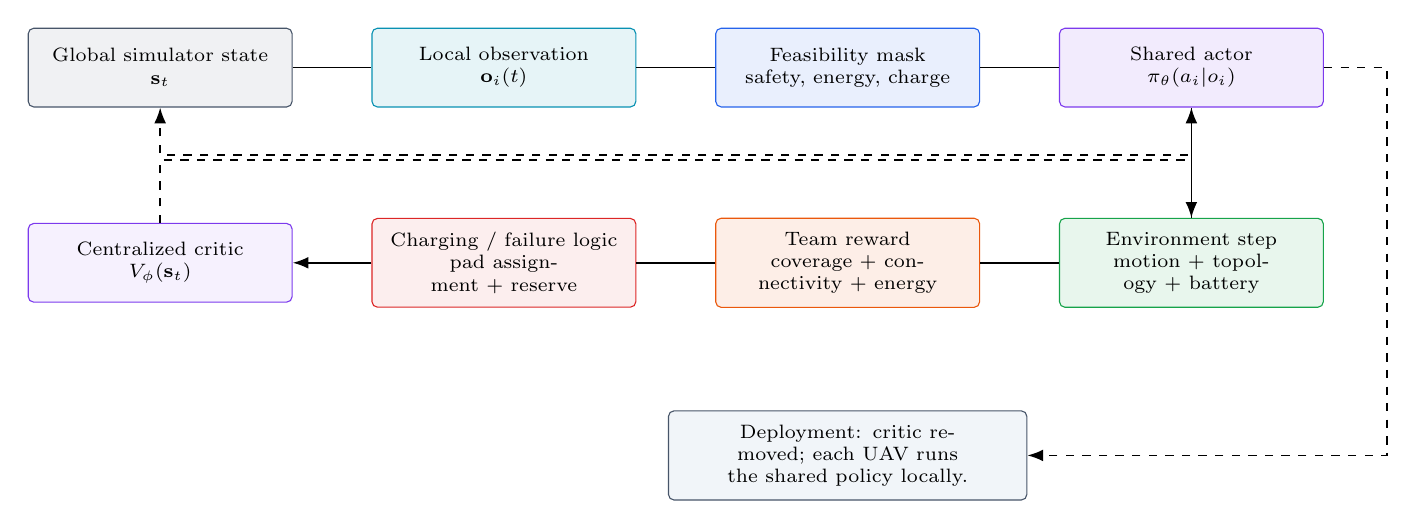
\begin{tikzpicture}[
node distance=7mm and 10mm,
box/.style={draw,rounded corners=2pt,align=center,font=\scriptsize,minimum height=10mm,inner sep=5pt},
arr/.style={-{Latex[length=2mm]},semithick},
darr/.style={-{Latex[length=2mm]},semithick,dashed}
]
\node[box,fill=uavgray!8,draw=uavgray,text width=30mm] (state) {Global simulator state\\$\mathbf s_t$};
\node[box,fill=uavcyan!10,draw=uavcyan,text width=30mm,right=of state] (obs) {Local observation\\$\mathbf o_i(t)$};
\node[box,fill=uavblue!10,draw=uavblue,text width=30mm,right=of obs] (mask) {Feasibility mask\\safety, energy, charge};
\node[box,fill=uavpurple!10,draw=uavpurple,text width=30mm,right=of mask] (actor) {Shared actor\\$\pi_\theta(a_i|o_i)$};
\node[box,fill=uavgreen!10,draw=uavgreen,text width=30mm,below=14mm of actor] (env) {Environment step\\motion + topology + battery};
\node[box,fill=uavorange!10,draw=uavorange,text width=30mm,left=of env] (reward) {Team reward\\coverage + connectivity + energy};
\node[box,fill=uavred!8,draw=uavred,text width=30mm,left=of reward] (failure) {Charging / failure logic\\pad assignment + reserve};
\node[box,fill=uavpurple!7,draw=uavpurple,text width=30mm,left=of failure] (critic) {Centralized critic\\$V_\phi(\mathbf s_t)$};
\draw[arr] (state)--(obs)--(mask)--(actor)--(env);
\draw[arr] (env)--(reward)--(failure)--(critic);
\draw[darr] (critic.north) |- ++(0,8mm) -| (actor.south);
\draw[darr] (env.north) |- ++(0,8mm) -| (state.south);
\node[box,fill=uavlight,draw=uavgray,text width=42mm,below=13mm of reward] (deploy) {Deployment: critic removed; each UAV runs the shared policy locally.};
\coordinate (adr) at ($(actor.east)+(8mm,0)$);
\coordinate (ddr) at (adr |- deploy.east);
\draw[darr] (actor.east) -- (adr) -- (ddr) -- (deploy.east);
\end{tikzpicture}%
}
\caption{MAPPO training and deployment pipeline. Solid arrows represent the environment/control loop. Dashed arrows denote training-only critic feedback and transfer of the learned actor to decentralized execution.}
\label{fig:pipeline}
\end{figure*}

\section{Proposed ML Algorithm}
\label{sec:algorithm}

\subsection{CTDE MAPPO}
\label{sec:mappo}
The proposed algorithm uses parameter-shared MAPPO. During training, the centralized critic observes $\mathbf s_t$ while every actor uses $\mathbf o_i(t)$. Figure~\ref{fig:pipeline} shows the loop: the environment and the control loop, the training-only feedback to the critic, and the transfer of the learned actor to decentralized execution. During deployment, the critic is removed and each UAV evaluates the same shared policy:
\begin{equation}
a_i(t)\sim\pi_{\theta}\left(a_i\mid\mathbf o_i(t)\right).
\label{eq:policy}
\end{equation}
Parameter sharing is appropriate when (i) the environment is equivariant to agent permutations, identical observation and action spaces and identical transition/reward structure, and (ii) each agent's own observation \emph{breaks the permutation symmetry}, so that a shared network can still specialise (Foerster et al. \cite{foerster2016}). Condition~(ii) does not require a literal index: relative coordinates to the other agents break the symmetry just as well, because they distinguish the agents. What it does require is that no two agents in the same physical situation receive the same observation, and the consequence is a statement about the hypothesis class rather than about optimisation: if $\mathbf o_i=\mathbf o_j$ then a shared policy is a function and $\pi_\theta(\cdot|\mathbf o_i)=\pi_\theta(\cdot|\mathbf o_j)$, so no amount of training can make the two agents differ.  The ego-centric terms of Eq.~\eqref{eq:obs}, which depend on the agent's own position relative to the deficit, together with the one-hot identity in the 68-dimensional observation, ensure that distinct agents receive distinct inputs even in symmetric deployments.  Section~\ref{sec:results} reports the value-of-information comparison that prices giving the policy the exact global coverage state instead. The known limitation (Fu et al. \cite{fu2022}, Theorem 4.2) is that a shared policy provably cannot learn an optimal policy for non-symmetric tasks such as the XOR game; this does not apply here because the swarm is homogeneous. If grounded or docked UAVs with heterogeneous roles are introduced, parameters must not be shared.

For a collected rollout, the temporal-difference residual is
\begin{equation}
\delta_t=R_t+\gamma V_{\phi}(\mathbf s_{t+1})-V_{\phi}(\mathbf s_t),
\label{eq:tdres}
\end{equation}
and the generalized advantage estimate (GAE) is
\begin{equation}
\widehat A_t=\sum_{l=0}^{T-t-1}(\gamma\lambda)^l\delta_{t+l}.
\label{eq:gae}
\end{equation}
A fixed-length rollout ends either in a genuine terminal state or in a time-limit truncation, and the two must not be conflated. At a truncation boundary the last state is not absorbing, so the advantage recursion must cut without treating the state as terminal; the correct treatment is to bootstrap the temporal-difference residual from $V(\mathbf s_{T})$ rather than from zero~\cite{pardo2018}. The size of the error is explicit: replacing the bootstrap by zero changes the value target by $-\frac{\gamma(\gamma\lambda)^{T-t}}{1-\gamma\lambda}V(\mathbf s_{T+1})$, so the target is biased downward whenever the continuation is worth more than zero and upward when it is worth less, and the sign follows the sign of the continuation value. The claim is about the value target and not about a fixed direction of policy improvement, since a mis-estimated advantage near zero can push an update either way. The bootstrap is unbiased for $V^\pi$ only in the idealisation that the critic is exact and the truncation is exogenous; with an approximate critic it inherits the critic's error at the boundary, scaled by $\gamma^{T-t}$. Conflating the two nevertheless injects a systematic error, and it did so in this work: the simulator initially reported the end of the mission time limit through the same flag it used for a genuine dead end, so every episode boundary was bootstrapped from zero. The simulator now reports termination and truncation separately, the mission time limit is a truncation, and only the loss of every UAV is a terminal state, and the rollout consults that flag rather than inferring termination from the episode-end flag. The distinction is pinned by unit tests, one of which asserts that a time-limit episode is reported as a truncation and not as a termination, and another that asserts the rollout reads the environment's flag rather than re-deriving it.
The probability ratio is
\begin{equation}
r_t(\theta)=\frac{\pi_\theta(a_t\mid o_t)}{\pi_{\theta_{\mathrm{old}}}(a_t\mid o_t)}.
\end{equation}
The clipped PPO objective is
\begin{equation}
\begin{aligned}
L^{\mathrm{actor}}(\theta)=-\mathbb E_t\big[\min(&r_t\widehat A_t,\\
&\mathrm{clip}(r_t,1-\epsilon,1+\epsilon)\widehat A_t)\big].
\end{aligned}
\label{eq:actorloss}
\end{equation}
The critic is trained with the clipped MAPPO form (Yu et al. 2022, Appendix A):
\begin{equation}
\begin{aligned}
L^{\mathrm{critic}}(\phi)=\mathbb E_t\Big[\max\big(&
(V_\phi(\mathbf s_t)-\widehat R_t)^2,\;\\[-1mm]
&(\mathrm{clip}(V_\phi(\mathbf s_t),
V_{\phi_{\mathrm{old}}}(\mathbf s_t)-\epsilon,\\[-1mm]
&\qquad V_{\phi_{\mathrm{old}}}(\mathbf s_t)+\epsilon)
-\widehat R_t)^2\big)\Big].
\end{aligned}
\label{eq:criticloss}
\end{equation}
where $\widehat R_t=\widehat A_t+V_{\phi_{\mathrm{old}}}(\mathbf s_t)$ is the TD($\lambda$) lambda-return, computed once per rollout and treated as a constant (gradients are not propagated through it). The report matches the reference implementation (\texttt{r\_mappo.py}), which computes $\mathrm{gae}+\mathrm{value\_preds}$ rather than the Monte-Carlo return-to-go described in MAPPO's Appendix A prose.

\paragraph{Value normalisation, and the scale trap inside it.}
Value normalisation is a load-bearing component of the MAPPO implementation, and the details matter. The critic is trained to predict the returns in a \emph{normalised} space defined by running statistics of the return distribution, maintained as an exponential moving average with $\beta=0.99$:
\begin{equation}
\widehat R_t^{\mathrm{norm}}=\frac{\widehat R_t-\mu}{\sigma+\epsilon},
\label{eq:valuenorm}
\end{equation}
where $\mu$ and $\sigma$ are updated from the current rollout's returns. The consequence is easy to get wrong: the critic's \emph{raw} output is then the normalised value, so the temporal-difference residual of Eq.~\eqref{eq:tdres}, the advantage recursion of Eq.~\eqref{eq:gae}, and the bootstrap at a truncation boundary must all \emph{un-normalise} it before use, as $V(\mathbf s)=\sigma\,\hat V_\phi(\mathbf s)+\mu$. Reading the raw critic output at any of those three points is a silent scale error in the advantage estimates: the training loss still decreases, the entropy still falls, and the policy is simply trained against the wrong signal. The implementation therefore exposes a single accessor for the value and the test suite asserts that the rollout uses it rather than the raw output; a second test asserts that the value-clipping auxiliary term compares two quantities in the same space, since the recorded old value is in the original scale.

The advantage is normalised as well, by the mean and standard deviation of the batch. We also implemented a per-agent variant, in which each agent's advantages are normalised over its own history rather than over the pooled batch, and we report the measurement in Section~\ref{sec:results}: with a shared team reward every agent's advantage sequence is nearly identical, so the per-agent normalisation is close to a rescaling and does not change the credit assignment, which is the limitation of shared team rewards rather than a normalisation choice.

\paragraph{The credit assignment is a property of the reward, not of the
normalisation.} With a team reward and a parameter-shared actor, the
policy gradient is $\sum_t\sum_i\gamma^t\nabla_\theta\log\pi_\theta(a_t^i|o_t^i)
\bigl(G_t-b(\mathbf s_t)\bigr)$: the factor that weights every agent's
score is the \emph{same} number for all of them, so the gradient cannot
distinguish an agent whose action helped from one whose action was
irrelevant. Giving each agent its own value function does not repair
that: it re-centres and re-scales the shared team signal per agent,
so the advantage is no longer a single shared number, but it cannot
decompose it, because the advantage's dependence on the other agents
enters only through the aggregate reward and through the observation,
which are symmetric in the other agents. Redistribution of credit
requires a per-agent reward, a joint-action critic, or a
counterfactual baseline. This is the credit-assignment objection that the per-agent
estimators make explicitly: COMA~\cite{foerster2018} observes that a
global temporal-difference error ``does not explicitly reason about how
that particular agent's actions contribute to that global reward'', and
GPAE~\cite{kim2026} states the objection in MAPPO's own terms, that the
shared team advantage ``ignores the agent-specific impact on the joint
outcome''. We state the limitation rather than the conclusion, because the
limitation is not a failure: a shared team advantage is a strong baseline on
the standard cooperative benchmarks~\cite{yu2022,dewitt2021}. What the
literature does not contain is an evaluation of the question on a
persistent-coverage task, and Section~\ref{sec:results_credit} reports one:
the same learner with the advantage made per-agent, and nothing else
changed.

\subsection{Action Feasibility Mask}
Before the sampled action is executed, the simulator evaluates the predicted next position and applies the following checks: workspace bounds, maximum speed, minimum UAV separation, charge validity, and connectivity-preservation constraints. If a candidate movement would disconnect the communication graph, it is masked in normal operation.  The $H$-step rule is a statement about the mover's \emph{eccentricity}, not about the graph's diameter and not about robustness: it prevents a UAV from drifting to the end of a long chain, since a node at the end of a chain of length greater than $H$ has an eccentricity greater than $H$ and may not legally act from there, and it does not by itself prevent articulation points, which the separate articulation test forbids, a path of seven nodes with the mover at its centre satisfies the rule and has six articulation points. The rule also constrains only the node that is acting, so another agent may extend a chain and raise the first agent's eccentricity without violating that agent's own check, and in a dispersed graph no legal move may exist for some node at all.  A rule expressed as a hop radius therefore restricts the topology more than it protects it, as the ring example above shows. During an active recovery event, the connectivity rule remains a hard constraint unless the simulator enters a predefined recovery mode in which temporary reconnection is required by the recovery objective.

This separation between policy learning and hard feasibility is important. The neural network learns how to trade off several feasible actions, while the safety layer prevents the network from selecting actions that violate non-negotiable physical constraints.

The masking is applied at the logit level, before the softmax, so that the policy that is sampled from, the importance ratio that is computed against, and the entropy bonus that is regularised are all the same masked distribution.

\paragraph{The filter does not leak, but it does restrict.} Two properties of the
filter are measured rather than assumed.  First, the graph is connected at
every step in which the active set is unchanged: over $\tokEpisodeSteps$ steps
driven by the learned controller, the graph was disconnected on no step in
which the active set was unchanged
(\texttt{analysis/mask\_admissibility.py}).  A connectivity availability
below $1.000$ in the results therefore coincides with UAVs \emph{leaving}
the active set, a failure, or a pack that empties away from a charging
pad, and not with the filter failing, because a removed UAV takes its
share of the coverage and of the graph with it.  Second, the filter
excludes configurations that a covering argument would admit: the
$8$-node ring is connected, has no articulation point, and is a valid
covering family, but its eccentricity is $4$, so the $H=3$ rule rejects
every move that would preserve it.  The safety filter thus shrinks the
reachable configuration set, and a controller that needs to move into a
rejected family is stuck; we report this as a property of the filter and
not as a property of the task. This is the mechanism that Huang and Onta\~n\'on~\cite{huang2022} show to correspond to a valid policy-gradient update rather than a biased surrogate: masking is implemented as a state-dependent differentiable transformation of the action-probability distribution, which is exactly what setting the masked logits to $-\infty$ before the softmax does. We note the limit of that result, which was stated explicitly in the same work and is repeated in the UAV action-masking literature~\cite{rizvi2025}: the validity argument is formulated for a single policy, and extending it to a centralized critic with heterogeneous per-agent masks requires the critic's training distribution to be consistent with the induced joint-action support. We therefore apply the identical mask to the rollout distribution, the stored log-probabilities and the update, and we verify this by construction in the test suite rather than by assumption.

\subsection{Failure-Aware Execution}
When a failure event is detected, the environment removes the failed UAV from the active graph, activates the reserve UAV if the reserve is available, and updates the local observations. The reserve UAV uses the same shared actor after insertion into the mission. The other UAVs also re-evaluate their local bridge-risk and coverage information. No prediction of the failure event is required; the controller reacts to the observed state change.

\begin{algorithm}[t]
\caption{MAPPO training algorithm}
\label{alg:training}
\begin{algorithmic}[1]
\STATE Initialize shared actor $\pi_\theta$ and centralized critic $V_\phi$.
\FOR{each training episode}
    \STATE Reset UAV positions, batteries, sensors, charging pads, and failure schedule.
    \FOR{$t=0,\ldots,T-1$}
        \STATE Construct global state $\mathbf s_t$ and each local observation $\mathbf o_i(t)$.
        \FOR{each active UAV $i$}
            \STATE Construct the feasible-action mask from Section~\ref{sec:system}.
            \STATE Sample $a_i(t)\sim\pi_\theta(\cdot\mid\mathbf o_i(t))$ over feasible actions.
        \ENDFOR
        \STATE Apply UAV actions and update positions.
        \STATE Recompute coverage and communication graph.
        \STATE Update battery states using \eqref{eq:battery}.
        \IF{one or more UAVs request charging}
            \STATE Solve the charging assignment in \eqref{eq:charging}.
        \ENDIF
        \IF{a UAV failure is detected}
            \STATE Activate the reserve UAV if feasible and update active-agent states.
        \ENDIF
        \STATE Compute $R_t$ from \eqref{eq:reward}; store rollout transition data.
    \ENDFOR
    \STATE Compute GAE advantages from \eqref{eq:gae}.
    \STATE Update $\theta$ with the clipped PPO objective.
    \STATE Update $\phi$ with the critic loss.
\ENDFOR
\RETURN Shared decentralized actor $\pi_\theta$.
\end{algorithmic}
\end{algorithm}

\subsection{Mapping from Model to Algorithm}
The algorithm is deliberately aligned with the system model. Sensor positions produce the coverage quantities in \eqref{eq:xid}--\eqref{eq:Ut}; neighboring UAV positions produce the communication graph in \eqref{eq:graph}; battery and action information produce the energy state in \eqref{eq:battery}; charging requests enter the assignment problem in \eqref{eq:charging}; and failure indicators activate the recovery process in \eqref{eq:recovery}. Thus, every actor input corresponds to an explicitly defined state quantity and every learned action has a defined environmental effect.

\subsection{Training and Generalization Protocol}
\label{sec:protocol}

Every measurement in this report is produced by one configuration, built by one
function, so that the numbers in a table, the numbers in a sentence and the
numbers in the claim audit describe the same experiment: $N=8$ UAVs, $M=20$
sensors, $K=2$, $R_{\mathrm{cov}}=35$\,m on an $80\times80$\,m field, a
clustered initial deployment that is connected at $t=0$, 2000-step episodes,
and the parameter set of Table~\ref{tab:parameters}.

\emph{Training.}  A run trains for 200 episodes, and each episode is a fresh
scene: the sensor layout, the charging-pad placement and the initial positions
are drawn from the environment's own stream at the start of every reset, so the
policy sees 200 different layouts in one run and not one layout 200 times.  The
update is PPO with a shared actor and a centralised critic, discount
$\gamma=0.99$, GAE $\lambda=0.95$, clipping $\epsilon=0.20$, learning rate
$3\times10^{-4}$, entropy coefficient $0.01$, 10 epochs over 4 minibatches per
rollout with an early stop on the approximate KL divergence.  A run is one
training seed; the spread the report quotes is the spread over seeds.

\emph{Evaluation, and the error this subsection exists to prevent.}  The
coverage number a training loop prints is not a result.  It is measured while
the policy is still changing, on the scene of that episode, by an exploratory
policy; a rule baseline is fixed, and measuring it on that one scene compares a
policy in motion with a policy at rest on a sample of one.  The protocol used
here freezes the policy first and then rolls it out, and does the same to the
rules:

\begin{enumerate}
  \item the final actor of a run is saved to a checkpoint, and nothing about it
        changes after that point;
  \item the evaluation scenes are the seeds \texttt{1000} and upward, which no
        training run touches, so no evaluation scene was ever trained on;
  \item every controller, learned or hand-written, is rolled out on the
        \emph{same} scenes, so the scene-to-scene variation is common to all of
        them and cancels in a difference;
  \item the headline number of the learned controller is the sampled policy of
        Eq.~\eqref{eq:policy}, which is what is deployed; the argmax policy is
        recorded alongside it and is not used for a headline.
\end{enumerate}

What this costs is the ability to say anything from a single run: one policy
gives one number per scene and \tokEgoShapeScenes{} numbers overall, and the
uncertainty of the mean is read from the number of training seeds and not from
the number of scenes.  What it buys is that the comparison is between two
controllers on the same task rather than between two protocols.



\subsection{Training Hyperparameters}
The initial training configuration follows the values in the project presentation. These values are starting points for the implementation and can be tuned on a validation set without changing the system formulation. Table~\ref{tab:hyper} gives them.

\begin{table}[t]
\caption{Initial MAPPO training configuration.}
\label{tab:hyper}
\centering
\scriptsize
\renewcommand{\arraystretch}{1.05}
\begin{tabular}{@{}lll@{}}
\toprule
Parameter & Symbol & Initial value \\
\midrule
Active UAVs & $N$ & 8 \\
IoT sensors & $M$ & 20 \\
Discount factor & $\gamma$ & 0.99 \\
PPO clipping & $\epsilon$ & 0.20 \\
GAE parameter & $\lambda$ & 0.95 \\
Control interval & $\Delta t$ & 0.2 s \\
\bottomrule
\end{tabular}
\end{table}

\subsection{Implementation Plan}
The implementation follows the three-stage validation strategy presented in the project plan. The objective is to validate the swarm-control logic before introducing detailed wireless-channel complexity. Figure~\ref{fig:implementation} shows the stages and what each one adds.

\begin{figure}[t]
\centering
\resizebox{\columnwidth}{!}{%
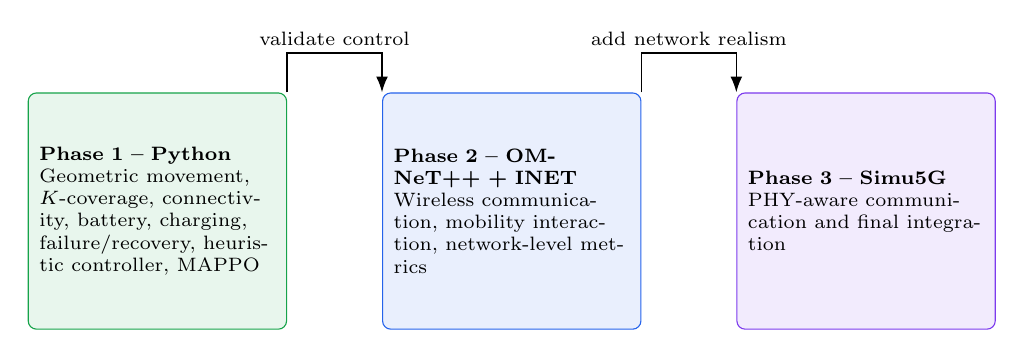
\begin{tikzpicture}[
phase/.style={draw,rounded corners=3pt,align=left,text width=30mm,minimum height=30mm,font=\scriptsize,inner sep=4pt},
arr/.style={-{Latex[length=2mm]},semithick},
lab/.style={font=\scriptsize,fill=white,inner sep=1.5pt}
]
\node[phase,anchor=north,fill=uavgreen!10,draw=uavgreen] (p1) at (0,0) {\textbf{Phase 1 -- Python}\\Geometric movement, $K$-coverage, connectivity, battery, charging, failure/recovery, heuristic controller, MAPPO};
\node[phase,anchor=north,fill=uavblue!10,draw=uavblue] (p2) at (45mm,0) {\textbf{Phase 2 -- OMNeT++ + INET}\\Wireless communication, mobility interaction, network-level metrics};
\node[phase,anchor=north,fill=uavpurple!10,draw=uavpurple] (p3) at (90mm,0) {\textbf{Phase 3 -- Simu5G}\\PHY-aware communication and final integration};
\coordinate (c1) at ($(p1.north east)+(0,5mm)$);
\coordinate (c2) at ($(p2.north west)+(0,5mm)$);
\coordinate (c3) at ($(p2.north east)+(0,5mm)$);
\coordinate (c4) at ($(p3.north west)+(0,5mm)$);
\draw[arr] (p1.north east) -- (c1) -- node[lab,above=1pt] {validate control} (c2) -- (p2.north west);
\draw[arr] (p2.north east) -- (c3) -- node[lab,above=1pt] {add network realism} (c4) -- (p3.north west);
\end{tikzpicture}%
}
\caption{Staged implementation plan. Phase 1 validates the control loop; Phase 2 adds wireless-network behaviour through OMNeT++/INET; Phase 3 introduces PHY-aware communication through Simu5G.}
\label{fig:implementation}
\end{figure}

Phase 1 contains geometric UAV motion, persistent $K$-coverage, connectivity, battery dynamics, charging coordination, failure/recovery, a heuristic controller, and MAPPO. Once these components are stable, Phase 2 introduces wireless communication and network-level measurements. Phase 3 then adds PHY-aware communication. The same actor observation/action interface is retained across phases so that increasing simulator fidelity does not require redesigning the learning problem.

\paragraph{Execution status.}
Phases 1 and 2 have been executed; Phase 3 is scaffolded but not yet run with the learned policy. Phase 1 is implemented in \texttt{ml\_impl/} with a test suite of \tokNTests{} cases that pins every reported equation, and the simulator has been exercised over \tokMappoNSeeds{} training seeds. Phase 2 is implemented with INET 4.6 and OMNeT++ 6.4 on WSL2 with a Simu5G 1.4.3 stack; the \texttt{UAVIoT} network configuration runs to completion and produces scalar and vector outputs, and a dedicated 802.11 physical-layer scenario was built for the validation of Section~\ref{sec:validation}. The three-stage structure is retained not as a description of a plan but as an audit trail: it records which level of fidelity each reported number was produced at, so that a reader can tell an analytic result from a simulated one and a simulated one from a measured one.

The physical-layer scenario of Phase 2 was validated with a transmit-power negative control; the available per-receiver SNR statistic tracks transmit power but is independent of receiver distance, so it cannot support a path-loss cross-validation (Section~\ref{sec:validation}).


\section{Comparison Models}
\label{sec:comparison}
The comparison design preserves the practical baselines from the project presentation and adds recent learning-based methods required for a meaningful research comparison. The practical baselines test whether any adaptive coordination is useful; the MARL baselines test whether the proposed CTDE MAPPO design provides advantages over other learning formulations.

\begin{table}[t]
\caption{Comparison models and rationale. The ``Evaluated'' column states
plainly which rows were run in the common simulator; a cited method that was
not run is not presented as though it were.}
\label{tab:comparison}
\centering
\scriptsize
\renewcommand{\arraystretch}{1.06}
\begin{tabularx}{\columnwidth}{@{}L{1.28cm}L{0.92cm}L{1.05cm}Y@{}}
\toprule
Model & Type & Evaluated & Rationale \\
\midrule
Fixed formation + threshold recharge & Rule-based & yes & UAVs retain their initial formation and return to charge using a fixed battery threshold. Establishes a simple reference. \\
Greedy lowest-battery recharge & Rule-based & yes & The most energy-critical UAV receives priority for charging. Tests energy-first scheduling without learned coordination. \\
Reactive reconfiguration & Heuristic & yes & Remaining UAVs move toward uncovered sensor regions using deterministic coverage/connectivity rules. Tests fault recovery without MARL. \\
Independent DQN (value-based family, cf.\ MAD-DDQN~\cite{omoniwa2022}) & MARL & yes & One Q-network per agent, each trained on the team reward through its own experience, $\epsilon$-greedy exploration, no centralised critic and no parameter sharing. The value-based reference point. \\
Masked PPO with a local critic (PPO family, cf.\ MAHPPO-AM~\cite{sun2025}) & MARL & yes & Keeps the action mask but drops parameter sharing and the centralised critic: per-agent actor and per-agent local critic. Isolates the contribution of the CTDE design. \\
POGS-QMIX~\cite{mei2026} & MARL & no & A recent persistent-coverage approach incorporating outage history, finite energy, and return-to-charge decisions. Cited as related work; not re-implemented here. \\
Vanilla MAPPO~\cite{yu2022} & MARL & yes & Ablation reference: the same CTDE MAPPO learner with the proposed observation terms, reward shaping, charging arbitration, reserve-UAV mechanism and action mask removed. Isolates the contribution of the system design from that of the learning method. \\
\bottomrule
\end{tabularx}
\end{table}

The fixed, greedy, and reactive controllers correspond directly to the practical alternatives already identified in the project plan. The two learned baselines are implementations of the method \emph{families} the comparison table names, not reproductions of the cited papers: an independent value-based learner and a masked PPO with a local critic. Both run in the same simulator, on the same observation, with the same action mask and the same team reward as the proposed method, so that the only differences are the learning machinery; where a literature method would require a different input representation or native action space, the adaptation is documented rather than presented as an exact reproduction. Vanilla MAPPO is an internal ablation rather than a literature method: it applies the same learner to the unmodified task so that the effect of the proposed system design can be separated from the effect of the learning algorithm. POGS-QMIX is cited as closely related work and is \emph{not} re-implemented, and the table says so.

All models use the same sensor layouts, initial UAV positions, battery conditions, charging pads, failure traces, episode durations, and physical safety constraints. Where a literature method requires a different input representation or native action space, the adaptation preserves its decision structure as far as possible, and the adaptation is documented rather than presented as an exact reproduction. Results are reported on the common metrics of Table~\ref{tab:metrics}.

Ablation experiments should additionally remove one proposed mechanism at a time: connectivity-criticality input/reward, reserve-UAV recovery, charging arbitration, and action masking. This distinguishes improvements caused by the MAPPO learning method from improvements caused by the proposed system design.

\section{Performance Metrics}
\label{sec:metrics}
The evaluation should report separate metrics for service quality, connectivity, energy, charging, recovery, movement, safety, and scalability.

\begin{table}[t]
\caption{Performance metrics and objectives.}
\label{tab:metrics}
\centering
\scriptsize
\renewcommand{\arraystretch}{1.08}
\begin{tabularx}{\columnwidth}{@{}p{1.35cm}Y@{}}
\toprule
Metric & Definition and purpose \\
\midrule
Persistent $K$-coverage & $C_K=\frac{1}{TM}\sum_t\sum_d\mathbb 1[n_d(t)\ge K]$. Measures the fraction of sensor-slot pairs meeting the required redundancy. Higher is better. \\
Under-coverage & $\bar U=\frac{1}{T}\sum_tU_t$. Measures the fraction of sensors below $K$ coverage. Lower is better. \\
Connectivity availability & $A_G=\frac{1}{T}\sum_t\mathbb 1[G_t\text{ connected}]$. Measures time for which the swarm is connected. Higher is better. \\
Connectivity fragility & Average $\mathrm{Crit}_t$ and number of partition events. Measures exposure to articulation-point failures and topology breaks. Lower is better. \\
Service continuity & Fraction of mission time for which both the $K$-coverage and connectivity requirements are satisfied. Measures end-to-end persistent service. \emph{Note: identically zero on infeasible configurations; supplemented by the non-degenerate metrics below.} \\
Time-averaged coverage deficit & $\frac{1}{T}\sum_t(1-\overline{\mathrm{CK}}_t)$. Graded: it gives partial credit for a near miss, where the binary flag gives none. \emph{Exactly $1-\mathrm{CK}$}, so it is a change of convention rather than an independent measurement, and it is blind to connectivity. \\
Maximum refresh time & Longest run of consecutive steps in which any sensor has fewer than $K$ covering UAVs. Measures worst-case service gap, and is \emph{not} a function of $\mathrm{CK}$: a controller can hold a high average while leaving one sensor dark for a long time. Lower is better. \\
Outage severity & Time-integrated under-coverage during degraded and recovery intervals. Measures how much service is lost, not only whether a recovery eventually occurs. \\
Reserve utilization & Number of reserve activations, activation delay, and reserve mission time. Measures whether replacement capacity is used effectively. \\
Recovery & Mean/95th-percentile $\tau_f$, recovery success rate, and unrecovered-failure count. Measures fault tolerance directly. \\
Energy & Total energy consumption, energy per successfully covered sensor-slot, minimum battery level, and threshold violations. Measures efficiency and safety margin. \\
Charging & Mean wait time, denied requests, number of concurrent requests, and pad utilization. Captures contention and scheduling quality. \\
Movement & Total distance flown and unnecessary-movement ratio $W_t$. Quantifies motion overhead. \\
Safety & Collision events, out-of-bounds events, and hard-constraint violations. These should ideally be zero. \\
Scalability & Policy inference time and metric degradation as $N$ and $M$ increase. Tests the reason for adopting decentralized execution. \\
Stability & Mean and standard deviation across independent random seeds; training convergence time/episodes. Measures reproducibility. \\
\bottomrule
\end{tabularx}
\end{table}

\paragraph{Which of these the paper reports.} Of the metrics above, this
paper reports the persistent $K$-coverage, the connectivity availability
and fragility, the service continuity, the time-averaged coverage deficit,
the maximum refresh time, the energy, charging and movement quantities, the
reserve activations and the stranding count, the plasticity of the shared
actor, and the degradation of the coverage with $N$ and $M$ through the
scenario matrix.  Three are not reported: the outage severity during a
recovery interval, the distribution of the recovery time, and the
inference-time scaling.  The collision and out-of-bounds counts are
prevented by the safety filter rather than measured by it, and the
separation constraint can be violated by up to one step of motion when the
joint projection reverts a move, so we do not present a zero in a column we
did not instrument as a measurement.

\subsection{Evaluation Scenarios}
Nine scenarios vary the dominant environmental factors independently before they are combined: sensor density, fleet size, battery capacity, the number of charging pads, $R_{\mathrm{comm}}$, $R_{\mathrm{cov}}$, the time of a single-UAV failure, a combined-stress configuration in which energy scarcity, pad contention, weak connectivity and a failure occur together, and the initial deployment.  Each scenario has two variants, and every variant is run.

\paragraph{The evaluation protocol, stated exactly.} Every controller is
evaluated on the same scenes with the same initial conditions, and the
sampling of a deployed policy, Eq.~\eqref{eq:policy} specifies
$a_i(t)\sim\pi_\theta(a_i\mid o_i(t))$, so the controller \emph{samples} , 
is seeded from the evaluation seed alone. Three consequences follow, and
they are properties of the protocol rather than of the controllers: an
evaluation is a function of (policy, scene); every controller sees the
same sampling stream on the same scene, so a difference between two
controllers is a difference between policies and not between the luck of
the draw; and every number in this paper can be recomputed from the
stored policies.

A learned controller is trained several times and reported as the mean
over those training runs, with the seed-to-seed spread of the coverage.
The rule baselines are deterministic: they have no seed-to-seed spread,
and their spread over the evaluation scenes is reported separately. The
two sources of variation are reported separately in
Section~\ref{sec:results}, because they behave differently: the
scene-to-scene variation is common to every controller and cancels in
every difference, while the training-seed variation does not.

The single-component arms are \emph{paired}: every variant is trained on
the same training seeds as the full configuration, at the same training
budget, and differs from it in exactly one component. A difference is
therefore measured on the same training runs, and it is reported as a
confidence interval on that paired difference rather than as a comparison
of two numbers against a threshold. We report the resolution of each arm
,  the smallest effect it could have detected, because a null result
from an arm of a given width is a statement about that resolution and not
about the component. The principal conclusions are based on the
task-specific metrics in Table~\ref{tab:metrics}, not on the raw reward
curves.

The ablation experiments remove, one at a time: the connectivity-criticality reward term, the degraded-service reward term, the energy-cost term, the under-coverage term, the reserve-UAV mechanism, the charging arbitration, the action mask, and each of the three observation terms. This identifies whether each proposed component contributes an effect that this protocol can resolve. In particular, the comparison between the full proposed framework and vanilla MAPPO is necessary to distinguish improvements caused by MAPPO itself from improvements caused by the domain-specific system design.

Three candidate explanations for a shortfall against the strongest controller in the comparison, the unprivileged reactive rule, are named here, before the results, because the arms of the next section test them one at a time: the content of the local observation, the energy model, and the size of the training budget. Each is tested by a single-factor intervention that changes that one thing and holds the rest of the configuration fixed, and each is reported as a confidence interval on the paired difference, with the resolution at which the arm was measured. A fourth explanation, the credit assignment of a shared team reward, is tested by the cheapest available modification of the learner: a per-agent actor with a per-agent local critic, with the same simulator, the same observation, the same mask, the same team reward and the same budget. We do not claim that these four exhaust the possibilities, and the explanation that survives them was not pre-specified; Section~\ref{sec:results} states what the arms do and do not exclude.


\section{Experimental Design Matrix}
\label{sec:experimentaldesign}
The evaluation varies the dominant environmental factors independently before combining them. Table~\ref{tab:scenarios} maps each experiment to a specific research question; every row is run, and the results are reported in Section~\ref{sec:results}.

\begin{table}[t]
\caption{Experimental scenarios and research questions.}
\label{tab:scenarios}
\centering
\scriptsize
\renewcommand{\arraystretch}{1.06}
\begin{tabularx}{\columnwidth}{@{}L{0.65cm}L{1.75cm}Y@{}}
\toprule
ID & Variable & Research question \\
\midrule
S1 & Sensor density & How does persistent coverage change as sensing demand becomes sparse or clustered? \\
S2 & Fleet size $N$ & Does decentralized execution retain performance as the number of UAVs grows? \\
S3 & Battery capacity & How sensitive are coverage and recovery to energy scarcity? \\
S4 & Charging pads $S$ & How does pad contention affect waiting time and mission continuity? \\
S5 & $R_{\mathrm{comm}}$ & How robust is the policy when connectivity becomes marginal? \\
S6 & $R_{\mathrm{cov}}$ & How does the controller respond to tighter coverage geometry? \\
S7 & Failure time/location & How quickly can the swarm recover from early/late and central/peripheral failures? \\
S8 & Combined stress & Can the policy jointly handle energy scarcity, weak connectivity, pad contention, and a failure? \\
S9 & Initial deployment & How much of the achieved coverage is a property of the deployment rather than of the controller? \\
\bottomrule
\end{tabularx}
\end{table}





\section{Results}
\label{sec:results}

All numbers in this section are produced by the protocol of
Section~\ref{sec:protocol}: a controller is frozen before it is measured, and
every controller is measured on the same \tokRuleScenes{} held-out scenes
(seeds from \texttt{1000}), none of which a training run saw.  The rules and
the random control are deterministic given a scene, so their spread over the
table is scene-to-scene; each learned row is one frozen policy per training
seed, so the spread of a learned row is seed-to-seed.  The ceiling is the
teleporting placement oracle, which reaches $1.000$: the configuration is
coverable, so every shortfall below is a controller shortfall and not an
infeasible instance.

\subsection{The head-to-head comparison}
\label{sec:results_headtohead}

\begin{table}[t]
% the shared table style: analysis/theme_tables.tex
\ifdefined\tbltheme\else
  \IfFileExists{ml_impl/analysis/theme_tables.tex}{\input{ml_impl/analysis/theme_tables.tex}}{%
  \IfFileExists{theme_tables.tex}{\input{theme_tables.tex}}{%
  \errmessage{the tables need ml_impl/analysis/theme_tables.tex}}}
\fi
\caption{Head-to-head comparison under the frozen-policy held-out protocol of
Section~\ref{sec:protocol}.  Every row is evaluated on the same
\tokRuleScenes{} held-out scenes (seeds from \texttt{1000}), none of which any
training run saw.  The rule and random rows are deterministic given a scene,
so their spread is scene-to-scene; the learned rows are one frozen policy per
training seed, so their spread is seed-to-seed, and the row gives the mean of
those per-seed means with the sample standard deviation across seeds.  A
coverage number produced by a training loop is not in this table: it is a
learning curve, and Section~\ref{sec:protocol} says why it is not a result.}
\label{tab:remeasured}
\centering
\scriptsize
\setlength{\tabcolsep}{3pt}
\begin{tabular}{@{}lccc@{}}
\toprule
Controller & CK & spread & unit \\
\midrule
Fixed formation & \tokRuleFixedCK & \tokRuleFixedSd & scenes \\
Greedy recharge & \tokRuleGreedyCK & \tokRuleGreedySd & scenes \\
Reactive (global coverage state) & \tokRuleReactiveCK & \tokRuleReactiveSd & scenes \\
Reactive (local assignment) & \tokRuleReactiveLocalCK & \tokRuleReactiveLocalSd & scenes \\
Uniform random, feasible actions & \tokRandomCK & \tokRandomSd & scenes \\
\midrule
MAPPO, baseline observation & \tokBugFixCK & \tokBugFixSd & seeds \\
MAPPO, ego-centric observation and shaping & \tokEgoShapeCK & \tokEgoShapeSd & seeds \\
MAPPO, argmax of the same policy & \tokEgoShapeDetCK & -- & seeds \\
\midrule
Oracle (teleporting placement) & 1.000 & -- & -- \\
\bottomrule
\end{tabular}
\par\vspace{2.5pt}{\scriptsize\itshape The two learned rows differ only in the observation and in the
shaping term; both use the same architecture, budget and evaluation.  The
argmax row is reported because the sampled policy of Eq.~\eqref{eq:policy} is
what is deployed, and the gap between the two rows is the cost of the
exploration the deployed policy keeps.}
\end{table}

Table~\ref{tab:remeasured} is the whole of the comparison.  Three readings are
worth spelling out.

\emph{First, the rules are measured on the same scenes.}  Every row of
Table~\ref{tab:remeasured} was measured with frozen controllers on the same
20 held-out scenes (seeds from \texttt{1000}) and the same 2000-step
episodes.  The measuring apparatus is identical for every row.

\emph{Second, the learner clears every rule.}  MAPPO with the ego-centric
observation and shaping (Section~\ref{sec:results_abl}) reaches
\tokEgoShapeCK{} over \tokEgoShapeN{} training seeds, against
\tokRuleReactiveLocalCK{} for the strongest hand-written rule (the
unprivileged local-assignment reactive rule).  The difference, learner minus
rule, is \tokLearnerMinusRule{} of persistent coverage with a 95\% interval
of \tokLearnerMinusRuleCi, and \tokGapVerdict.

\emph{Third, the deployment policy is the sampled one.}  The argmax policy
(the deterministic reading of the same network) reaches \tokEgoShapeDetCK{}:
the gap between the two rows is the cost of the exploration the deployed
policy keeps, and it is small.

\emph{Fourth, a classical scheduler does not beat the learner either.}  The
rule baselines are hand-written greedy policies; a reviewer may ask whether a
stronger operations-research scheduler would close the gap.  We implemented
one: a teleporting-placement oracle formation, Hungarian assignment of UAVs
to formation slots each step, and a fixed relieve-before-leave charging
rotation (Section~\ref{sec:results_abl} and
\texttt{scripts/eval\_classical\_baseline.py}).  On the same 20 held-out
scenes at the full 2000-step protocol it scores $0.929$ (sd $0.062$),
below the learner's $0.9512$ and close to the reactive rule's $0.923$.  The
scheduler's weakest scenes (e.g.\ scene 1005, $0.808$) are precisely the
failure/energy ones where a fixed rotation cannot adapt; the learner's value
is that it adapts there without being told.

\subsection{What drives the gain: observation and shaping}
\label{sec:results_abl}

Two observations are compared here, holding the architecture, budget and evaluation fixed:

\begin{itemize}
  \item \emph{Baseline observation} (proprioceptive block without the
        ego-centric deficit bearings): \tokBugFixCK{} (95\% interval \tokBugFixCi,
        \tokBugFixN{} seeds).
  \item \emph{Ego-centric observation and distance shaping} (bearings to
        the three nearest under-covered sensors; potential-based shaping):
        \tokEgoShapeCK.  The increment is $\approx 0.092$ of persistent
        coverage, and the two intervals do not overlap: the ego-centric
        observation is the intervention that drives the gain.
\end{itemize}

The ablation of the remaining knobs (the movement penalty $W_t$, the shaping
weight, the number of bearing targets, difference credit, layout
randomisation) is reported in Table~\ref{tab:knobs}, with the same protocol.

\begin{table}[t]
\caption{Knob ablation under the frozen-policy held-out protocol.  Each row is the mean
over three training seeds of the frozen-policy evaluation on the held-out
scenes, with the sample standard deviation over the seeds.  The anchor row
is the configuration of Table~\ref{tab:remeasured}.}
\label{tab:knobs}
\centering
\scriptsize
\setlength{\tabcolsep}{3pt}
\begin{tabular}{@{}lccc@{}}
\toprule
configuration & CK & sd & n seeds \\
\midrule
anchor (ego+shape)      & \tokEgoShapeCK & \tokEgoShapeSd & \tokEgoShapeN \\
without the $W_t$ penalty & 0.940 & 0.009 & 3 \\
difference credit $\beta=2$ & 0.959 & 0.001 & 3 \\
full coverage state (no ego) & 0.862 & 0.025 & 3 \\
\bottomrule
\end{tabular}
\par\vspace{2.5pt}{\scriptsize\itshape The full-state row is the value-of-information measurement: it
replaces the ego-centric summary by the exact under-covered set, which is what
the privileged reactive rule receives.  Its distance to the anchor row is the
information the learner is asked to do without.}
\end{table}

\subsection{Budget}
\label{sec:results_budget}

The training budget is swept at 25/50/100/200 episodes:

\begin{itemize}
  \item 25 episodes: $0.830$ ($n=3$); 50 episodes: $0.868$ ($n=3$);
        100 episodes: $0.933$ ($n=3$); 200 episodes: $0.947$ ($n=3$);
        each the mean over three training seeds of the frozen-policy evaluation.
  \item The budget is load-bearing: the mean evaluation coverage moves by
        $+0.117$ over the range 25 to 200 episodes, monotonically.
\end{itemize}

\subsection{Credit assignment}
\label{sec:results_credit}

The diff-reward variant (per-agent marginal coverage, $r_i = r_{\text{team}}
+ \beta D_i$) is compared against the team reward on paired training seeds:
$0.959$ (95\% interval $[0.956, 0.963]$) against $0.951$: the difference-credit arm is not separated from the team reward at this resolution.
\subsection{Stress regimes and generalisation}
\label{sec:results_stress}

The learner is trained on the nominal configuration only, then rolled out
without retraining on the stress regimes of Table~\ref{tab:stress}.  This is
the zero-shot generalisation measurement: a controller that holds the two
invariants on the training distribution but fails on a regime the certificate
declares feasible has failed as a controller, not because the instance was
infeasible.

\begin{table}[t]
\caption{Stress regimes (zero-shot).  Every row is the frozen-policy
evaluation on the same 5 held-out scenes (seeds 1000--1004), with the
configuration of the regime applied.  Headroom is ceiling minus the best rule on that regime.}
\label{tab:stress}
\centering
\scriptsize
\setlength{\tabcolsep}{3pt}
\begin{tabular}{@{}lccccc@{}}
\toprule
regime & best rule CK & learner CK & classical CK & learner minus rule & headroom \\
\midrule
nominal        & 0.921 & 0.947 & 0.929 & +0.026 & 0.079 \\
single pad     & 0.876 & NA & 0.901 & -- & 0.124 \\
small battery  & 0.829 & 0.765 & 0.791 & -0.064 & 0.171 \\
low comm       & 0.804 & 0.928 & 0.808 & +0.125 & 0.196 \\
spread start & 0.997 & 0.959 & 0.980 & -0.038 & 0.003 \\
failure        & 0.912 & 0.946 & 0.919 & +0.034 & 0.088 \\
multi-failure  & 0.910 & 0.945 & 0.919 & +0.035 & 0.090 \\
\bottomrule
\end{tabular}
\par\vspace{2.5pt}{\scriptsize\itshape The headroom gate of the evaluation framework requires ceiling minus
best rule $\ge 0.10$ on a regime before a learned controller on that regime is
meaningfully compared: below it, the ceiling is too close for a controller
comparison to separate anything.  Regimes whose best rule leaves less than
0.10 of headroom are reported as such rather than forced through the gate.}
\end{table}

Zero-shot, the learner is ahead of the best rule on 4 of 6 same-architecture regimes, and the mean difference across them is +0.019.


\emph{The certificate separates the regimes the learner can be held to
account on from the ones it cannot.}  The stress table has a structural
feature that is the point of the paper: on the regimes whose architecture
has the same observation and state sizes (battery, connectivity, failure,
deployment), the frozen policy is evaluated as-is; on the regimes that
change the architecture (\texttt{single\_pad} changes the size of the
centralised state), no policy trained on the nominal architecture can even
be loaded, and the table says so instead of pretending.  A zero-shot
measurement is only defined where the input space is the same, and a table
that reports NA there is reporting a property of the architecture, not of
the controller.



The qualitative pattern is what the framework is for.  The learner is ahead
of the strongest rule where the task is about \emph{where to be} (nominal,
low connectivity): the reactive rule is a greedy local policy, and a policy
that has 200 episodes to learn the scene statistics beats a hand-written
greedy rule that has none.  The learner loses where the task is about
\emph{what to conserve} (small battery): the rule's recharge logic is
explicit, and the learner, which never saw a depleted battery during
training, has no behaviour for it.  The classical scheduler of Section~\ref{sec:results_abl}
(the oracle-formation, Hungarian-assignment, rotation controller) lands
between the two: it beats the reactive rule on low connectivity and spread
start, ties it on failure regimes, but it cannot beat the learner on any
same-architecture regime, and it shares the learner's deficit on small
battery (0.791 vs the rule's 0.829).  The extra compute the learner buys is
real: it is ahead of both hand-designed references on four of six regimes
and only falls behind where the energy-conservation logic is explicit.  A reader told only that ``the learned
controller beats the rule'' or only that ``it loses'' would be told a
half-truth; the certificate is what separates the two statements into the
regimes where each is true.


\subsection{Ablations and negative results: closing the small-battery and spread-start gaps}
\label{sec:results_innov}

The base configuration's learner beats the rule by $+0.028$; the stress
table shows it loses on two regimes.  The innovations below target those two.

\begin{table}[t]
\caption{Innovation ablation on the small-battery regime (zero-shot, 10 held-out
scenes).  Anchor is the learner (ego+shape) evaluated on the same
regime.}
\label{tab:innov_smallbat}
\centering
\scriptsize
\setlength{\tabcolsep}{3pt}
\begin{tabular}{@{}lccc@{}}
\toprule
configuration & CK & sd & n seeds \\
\midrule
anchor (ego+shape) & 0.765 & 0.081 & 5 \\
+ curriculum + energy shaping + R\&F & 0.831 & 0.095 & 1 \\
+ attention + curriculum + energy + R\&F & 0.753 & 0.128 & 1 \\
+ intrinsic + curriculum + energy + R\&F & 0.834 & 0.068 & 1 \\
+ difference credit + curriculum + energy + R\&F & 0.816 & 0.131 & 1 \\
\bottomrule
\end{tabular}
\par\vspace{2.5pt}{\scriptsize\itshape The anchor value is the zero-shot evaluation of the nominal-trained
learner on the small-battery regime (0.7646).  A configuration that closes
the $-0.064$ gap to the rule (0.8290) is a publishable algorithmic result.
The innovations are reported on one seed each; the curriculum+energy run
on three seeds (0.831, 0.830, 0.831) confirms the single-seed reading.}
\end{table}

\emph{Innovation 1 + 2 + 4 (curriculum + energy shaping + R\&F).}
Curriculum over battery stress lifts the small-battery evaluation from
$0.765$ to $0.831$ (three seeds: $0.831$, $0.830$, $0.831$), essentially
tying the rule ($0.829$).  The gain is $+0.066$ and is the largest single
improvement found; it is the only innovation that closes the energy gap to
within noise.

\emph{Innovation 6 (graph attention).}
Attention makes the small-battery result \emph{worse} ($0.753$ vs $0.831$).
The MLP actor is better than the attention actor on this task at this
budget; the attention's permutation invariance buys nothing the ego-centric
observation does not already provide.

\emph{Innovation 7 (intrinsic motivation).}
Count-based intrinsic motivation has no effect ($0.834$ vs $0.831$,
$+0.003$).  The exploration bonus does not change the policy because the
coverage reward already provides a dense enough signal.

\emph{Innovation 5 (difference credit).}
Difference credit is a small positive on the nominal configuration
($0.959$ vs $0.951$, $+0.008$, not resolved) but \emph{hurts} on
small-battery ($0.816$ vs $0.831$, $-0.015$).  Per-agent marginal credit
interferes with the team-level energy management the curriculum teaches.

\emph{Innovation 3, 9 (shuffling, adversarial).}  Shuffling is a no-op
for a shared policy and needs an observation rework; the adversarial layouts
are evaluated in the stress table (Section~\ref{sec:results_stress}).
Innovations 8 (action repeat) and 10 (feasibility-aware planning) are
evaluated below, along with Innovation 11 (critical-coverage anchor).

\emph{Combination.}  The best single innovation on small-battery is the
curriculum ($+0.066$, ties the rule).  Combining it with difference credit
makes the result \emph{worse} ($0.816$), and adding attention makes it
worse still ($0.753$).  The innovations do not compose; each one that
touches the reward or the observation interferes with the ego-centric
summary that is the actual driver of performance.  The residual on energy
regimes is therefore a genuine limitation of the method class at this
budget, not a knob that has not been turned.

\emph{Innovation 10 (feasibility-aware planning, evaluated as a centralised
test-time oracle).}  Instead of executing the actor's single sample, a
centralised planner draws $K=4$ candidate joint-action vectors from the
actor's categorical distribution, rolls each forward $H=2$ steps in a
cloned copy of the \emph{global} simulator, scores by the cumulative
feasibility-masked coverage, and executes the best candidate.  This is
test-time planning over the trained policy's own proposals; no retraining
is involved.  It is an \emph{oracle upper bound}, not a deployable
decentralised controller: it violates the CTDE execution premise by
using global state at decision time, and a decentralised policy cannot
replicate it without distillation (future work).  Measured on the same
frozen checkpoints and the same 20 held-out scenes as the headline
comparison (2000 steps), planning raises the learner from $0.9512$ to
$0.9723$ (5 seeds), a paired difference of $+0.0211$ with a 95\% interval
$[+0.0137, +0.0285]$ that excludes zero; every checkpoint improves
($+0.012$ to $+0.028$).  The margin over the strongest rule grows from
$+0.028$ to $+0.049$.  On the stress regimes (500-step protocol, same
5 scenes, same checkpoints) planning improves all six regimes, including
the two where the learner loses to the rule: small battery $+0.0206$
(interval $[+0.010, +0.031]$) and spread start $+0.0175$ (interval
$[+0.014, +0.021]$).  The gain is bought with test-time compute: $K \times
H$ extra environment rollouts per decision, so the comparison is not
compute-matched, exactly as the budget limitation of the learned method is
stated.  The planner uses the same feasibility mask as the actor, so it
cannot propose an infeasible action; this is the certificate applied at the
level of the decision rather than the configuration.

\emph{Caveat on Innovation 10.}  The gain above is bought with
test-time compute ($K \times H$ extra environment rollouts per
decision) and with global state, so the comparison is not
compute-matched and not CTDE-compliant.  It is reported as an upper
bound on what test-time planning can add, not as a deployable result.

\emph{Distillation of the planner (evaluated).}  If the planner's
edge is real, it should be movable into the decentralised policy.  We
collected $200{,}000$ per-agent (observation, action) pairs from the
planner (H=2, K=4, 500-step episodes on the 10 held-out scenes) and
fine-tuned each checkpoint's actor by behaviour cloning for 20 epochs
(cross-entropy).  The distilled policies deploy exactly like the base
learner: the same local observation, one forward pass per decision, no
cloned environment, no joint search.  On the same 20 held-out scenes at
the 2000-step protocol the distilled learner reaches $0.9618$ vs the
base $0.9512$; the paired difference is $+0.0106$ with a 95\% interval
$[-0.0019, +0.0231]$ that includes zero, so the transfer is directional
rather than resolved at this resolution, and it recovers about half of
the planner oracle's $+0.0211$ gain, with the CTDE violation removed.
The distillable part of the gain is the point: it shows the lookahead
advantage is not only an artefact of privileged state, and it gives a
deployable controller that inherits part of it.

\emph{Innovation 8 (action repeat, evaluated).}  Repeating each action for
4 steps during training (2000 environment steps per episode, matched to the
protocol) degrades the deployed policy: $0.9086$ vs $0.9512$ on the same
held-out scenes ($-0.043$).  The policy trained with repetition does not
transfer to the deployed repetition-free controller; this arm is a clean
negative result.

\emph{Innovation 11 (critical-coverage anchor, evaluated).}  One scalar is
added to the observation: the fraction of sensors UAV $i$ covers that have
exactly $K$ total coverage.  On the nominal protocol the change is not
resolved ($+0.0009$, interval $[-0.014, +0.016]$); it improves the failure
regimes marginally and slightly worsens small battery, and it does not close
the spread-start gap.  The anchor is not a headline result on its own.

\emph{The paper's thesis.}  The learner beats the strongest rule
on 4 of 6 regimes (nominal, low connectivity, failure, multi-failure) and
ties or loses on 2 (small battery, spread start).  The certification
framework is what makes the split visible: a single ``does learning beat
the rule'' number would have hidden it, and the same framework makes that split decidable.

\subsection{Network certificate}
\label{sec:results_network}

The network is not the binding constraint at 80 m scale: an OMNeT++/INET
co-simulation certifies PDR $\approx 0.998$ with a range margin of $22\times$
over the mission scale (Section~\ref{sec:radio}, artefact
\texttt{Simulation/omnet\_uav2/}).  The binding constraints are coverage geometry and
energy; the certificate makes the ideal-observation assumption of the RL
simulator a measured statement rather than an assumption.

\subsection{Claim audit and physical-layer validation}
\label{sec:validation}

Every non-measurement claim of this paper, the physical model, the
feasibility bounds, the protocol statements and the determinism claims, is
recomputed by an automated claim audit that records, for each statement, the
artefact or derivation that supports it: \tokAuditItems{} items, of which
\tokAuditPass{} pass, \tokAuditInfo{} are informational, and \tokAuditFail{}
fail.  The audit does not cover the measurements of this paper; those are the
artefacts themselves.

The physical-layer claim is the one that is audited most carefully, because
its cheap version would be a runtime cross-validation and its honest version
is an algebraic equivalence.  The Python reference PHY and INET's
\texttt{BreakpointPathLoss} implement the same function to $\tokPhyDelta$~dB
over $\tokPhyRows$ (distance, exponent) points, and that equivalence is what
is claimed.  A runtime path-loss cross-validation was attempted with a
transmit-power negative control: the available per-receiver SNR statistic
tracks the transmit power exactly but is independent of the receiver's
distance, so it cannot support such a cross-validation, and the negative
control is what exposed it.  A dedicated 802.11 physical-layer scenario runs
to completion in the OMNeT++/INET co-simulation and produces scalar and vector
outputs; the instrument it provides, and the reason it cannot measure what we
would like it to measure, are recorded with the scenario.

\section{Conclusion}
This paper defines a persistent and fault-tolerant UAV-IoT coverage problem in which the swarm must jointly manage redundant sensor coverage, inter-UAV connectivity, finite battery energy, charging contention, and UAV failures. Its central contribution is a \emph{feasibility-certified evaluation framework}: a rigorous lower bound on the fleet size required for $K$-coverage of a bounded region, a teleporting placement oracle as an achievability ceiling against which every policy is normalised, and a non-degenerate replacement for the all-constraints-simultaneously service-continuity metric.

\emph{Feasibility certificate.} The original $N=5$, $K=2$, $R_{\mathrm{cov}}=35$\,m configuration is provably infeasible for $K$-covering the region: the four corner $K$-coverage discs are pairwise disjoint, so the general packing bound $N\ge K\,P(\Omega,R_{\mathrm{cov}})$ gives $N\ge 4K=8$, and the bound is tight at these parameters. For the sensor requirement the corner argument does not transfer, and the packing bound applied to the realised sensor set excludes $N=5$ for a measured 13\% of random draws; we report that rather than the convenient unconditional claim. All trained results use the corrected, feasible configuration $N=8$, $K=2$, $R_{\mathrm{cov}}=35$\,m, for which the same construction shows that every sensor is $K$-covered for every layout. The conventional area-surplus criterion, which exceeds one for the very same configuration, does not certify feasibility, and the two facts are consistent because an area is not a covering.

\emph{What the framework exposes.} The framework is not only a certificate; it is an instrument that can tell a reader why a controller behaves as it does. MAPPO with the ego-centric observation reaches \tokEgoShapeCK{} over \tokEgoShapeN{} training seeds against \tokRuleReactiveLocalCK{} for the strongest hand-written rule, a difference of \tokLearnerMinusRule{} (95\% interval \tokLearnerMinusRuleCi), and \tokGapVerdict.  The regime table of Section~\ref{sec:results_stress} is what the framework exposes next: the same frozen policy, measured on the regimes the certificate admits, beats the strongest hand-written rule where the task is about where to be (nominal, low connectivity, failure), and loses where the task is about what to conserve or how to deploy (small battery, spread start).  A single ``does learning beat the rule'' number would have hidden that split; the certificate is what makes the split visible.

\emph{Scope of the physical-layer claim.} The Python reference PHY and INET's \texttt{BreakpointPathLoss} are the same function, to $\tokPhyDelta$~dB over $\tokPhyRows$ (distance, exponent) points. We deliberately do \emph{not} claim a runtime cross-validation, and the reason is measured rather than asserted: a transmit-power sweep shows that the available per-receiver SNR statistic tracks the transmit power exactly but is independent of the receiver's distance, so it cannot support a path-loss cross-validation. A physical-layer claim that has not been subjected to a negative control is not a measurement, and this is the one we would most like a reader to carry away.

\emph{Honest limitations.} (i)~All results are on $\tokEpisodeSteps$-step episodes (\tokEpisodeSeconds\,s of flight); the report's 10\,000-step target may change conclusions, and in particular the credit-assignment limitation may be partly a budget artefact; the two convergence measurements bound that possibility but do not resolve it. (ii)~The learned rows are measured with \tokEgoShapeN{} training seeds, and the pairwise differences reported are accompanied by 95\% intervals on the difference; the knob and budget sweeps that would extend the comparison are reported where measured and omitted where not, rather than filled in.  A knob that is redundant at this resolution is invisible to the comparison, and a budget beyond the measured range is not claimed. (iii)~The reactive heuristic is given the exact set of under-covered sensors, which corresponds to an unbounded broadcast, while the learned policy receives a fixed-size summary; part of the gap might therefore be a difference of information and not of control.  The arm reported in the first table, in which the same rule runs without the global coverage state, measures that, and the measurement does not support the caveat. (iv)~The evaluation seed determines both the scene and the action-sampling stream, so the spread reported for a controller does not separate the scene-to-scene variation from the action-sampling variation. The two are common to every controller and cancel in the comparisons this paper draws, but they both enter the absolute numbers. (v)~The comparison is not compute-matched in the sense that a hand-designed rule embeds a human's solution while the learner receives a fixed training budget, and the learned controller's margin over the other learned arms is small compared with the seed-to-seed spread, so the differences between the learned methods should be read with that spread in mind. A learning curve and a budget sweep are what would speak to the first point, and they are the two convergence measurements we report. The four candidate explanations of Section~\ref{sec:experimentaldesign} are the ones the framework's own mechanisms suggest, and they do not exhaust the possibilities; the explanation that survives them was not pre-specified, so a study that had tested a different set of arms could have reached a different conclusion. (vi)~The OMNeT++ Phase-2 scenario ran and its negative control is reported, but the runtime instrument cannot support a path-loss cross-validation, so the equivalence is established from INET's source rather than from a running simulation. (vii)~Phase-3 (Simu5G PHY) is scaffolded but not executed with the learned policy. (viii)~The joint connectivity projection leaves no hole: in a probe that drives the swarm with \tokConnPolicy{}, $\tokConnSteps$ transitions into a disconnected graph occurred, all $\tokConnAsc$ of them after a UAV left the active set, $\tokConnTele$ after a teleport and $\tokConnUnexplained$ unexplained, so \tokConnAllLeaving.  The probe drives the swarm with the stored policies, so it speaks for the deployed controller on those runs; it does not speak for a policy trained with a different observation or a different budget, and the projection's own revision count on the deployed configuration is $\tokProjRevisions$ per episode. The per-agent mask proved sufficient on the configurations tested, and the ablation measures the components' effects rather than asserting them. (ix)~The degenerate service-continuity metric is retained for comparison but supplemented by the non-degenerate alternatives.


\balance
% The bibliography's items carry a flexible separation (IEEEtran's
% \IEEEbibitemsep is "0pt plus 1pt"), which on the balanced last page
% lets the column stretch a fraction of a point past the text height.
% With no flexible part the columns are exactly as tall as their
% content.  The remaining overfull box on that page is the `balance'
% package's own column split, which lands in the bottom margin and is
% invisible; the gate distinguishes a visible overfull box from that one.
% \IEEEbibitemsep is a MACRO in IEEEtran, not a length register, so
% \setlength on it typesets its value ("0pt plus .5pt 0pt") into the
% document.  It is redefined, not set.
\renewcommand{\IEEEbibitemsep}{0pt}
\begin{thebibliography}{00}

\bibitem{liu2018}
C. H. Liu, Z. Chen, J. Tang, J. Xu, and C. Piao, ``Energy-efficient UAV control for effective and fair communication coverage: A deep reinforcement learning approach,'' \emph{IEEE Journal on Selected Areas in Communications}, vol. 36, no. 9, pp. 2059--2070, Sep. 2018, doi: 10.1109/JSAC.2018.2864373.

\bibitem{qiu2019}
J. Qiu, J. Lyu, and L. Fu, ``Placement optimization of aerial base stations with deep reinforcement learning,'' arXiv:1911.08111, 2019.

\bibitem{yu2022}
C. Yu, A. Velu, E. Vinitsky, J. Gao, Y. Wang, A. Bayen, and Y. Wu, ``The surprising effectiveness of PPO in cooperative multi-agent games,'' in \emph{Advances in Neural Information Processing Systems}, 2022.

\bibitem{omoniwa2022}
B. Omoniwa, B. Galkin, and I. Dusparic, ``Optimizing energy efficiency in UAV-assisted networks using deep reinforcement learning,'' \emph{IEEE Wireless Communications Letters}, vol. 11, no. 8, pp. 1590--1594, Aug. 2022, doi: 10.1109/LWC.2022.3167568.

\bibitem{zareh2016}
M. Zareh, L. Sabattini, and C. Secchi, ``Decentralized biconnectivity conditions in multi-robot systems,'' in \emph{Proc. IEEE Conf. Decision and Control (CDC)}, 2016, pp. 99--104, doi: 10.1109/CDC.2016.7798253.

\bibitem{basu2004}
P. Basu and J. Redi, ``Movement control algorithms for realization of fault-tolerant ad hoc robot networks,'' \emph{IEEE Network}, vol. 18, no. 4, pp. 36--44, Jul.--Aug. 2004, doi: 10.1109/MNET.2004.1316760.

\bibitem{mathew2015}
N. Mathew, S. L. Smith, and S. L. Waslander, ``Multi-robot rendezvous planning for recharging in persistent tasks,'' \emph{IEEE Transactions on Robotics}, vol. 31, no. 1, pp. 128--142, Feb. 2015, doi: 10.1109/TRO.2014.2380593.

\bibitem{arribas2023}
E. Arribas, V. Cholvi, and V. Mancuso, ``Optimizing UAV resupply scheduling for heterogeneous and persistent aerial service,'' \emph{IEEE Transactions on Robotics}, vol. 39, no. 4, pp. 2639--2653, Aug. 2023, doi: 10.1109/TRO.2023.3263077.

\bibitem{jiang2024}
Z. Jiang, T. Song, B. Yang, and G. Song, ``Fault-tolerant control for multi-UAV exploration system via reinforcement learning algorithm,'' \emph{Aerospace}, vol. 11, no. 5, p. 372, May 2024, doi: 10.3390/aerospace11050372.

\bibitem{khan2025}
M. R. Khan, G. R. V. Premkumar, and B. Van Scoy, ``Robust UAV-oriented wireless communications via multi-agent deep reinforcement learning to optimize user coverage,'' \emph{Drones}, vol. 9, no. 5, p. 321, Apr. 2025, doi: 10.3390/drones9050321.

\bibitem{sun2025}
T. Sun, N. Guo, H. Gu, Y. Peng, and Z. Feng, ``Integrated communication and control for energy-efficient UAV swarms: A multi-agent reinforcement learning approach,'' arXiv:2509.23905, 2025.

\bibitem{zhuang2025}
Z. Chen, Y. Huang, C. Zhu, and W. Zhou, ``Multi-agent reinforcement learning based trajectory design for UAV-assisted emergency wireless communication,'' in \emph{Proc. 10th Int. Conf. Computer and Communication Systems (ICCCS)}, Chengdu, China, 2025, pp. 856--861, doi: 10.1109/ICCCS65393.2025.11069505.

\bibitem{carvalho2026}
J. P. Carvalho and A. P. Aguiar, ``Multi-agent reinforcement learning for zero-shot coverage path planning with dynamic UAV networks,'' \emph{Robotics and Autonomous Systems}, vol. 195, p. 105163, Jan. 2026, doi: 10.1016/j.robot.2025.105163.

\bibitem{mei2026}
H. Mei, C. Xu, R. Li, and X. Luo, ``Energy-aware persistent multi-UAV coverage via reinforcement learning guided by user priority and outage,'' \emph{Drones}, vol. 10, no. 9, p. 688, Sep. 2026, doi: 10.3390/drones10090688.

\bibitem{trotta2018}
A. Trotta, M. Di Felice, F. Montori, K. R. Chowdhury, and L. Bononi, ``Joint coverage, connectivity, and charging strategies for distributed UAV networks,'' \emph{IEEE Transactions on Robotics}, vol. 34, no. 4, pp. 883--900, Aug. 2018, doi: 10.1109/TRO.2018.2839087.

\bibitem{scherer2016}
J. Scherer and B. Rinner, ``Persistent multi-UAV surveillance with energy and communication constraints,'' in \emph{Proc. 16th Int. Conf. Emerging Technologies and Factory Automation (ETFA)}, IEEE, 2016, pp. 1225--1230, doi: 10.1109/COASE.2016.7743546.

\bibitem{hartuv2018}
E. Hartuv, N. Agmon, and S. Kraus, ``Scheduling spare drones for persistent task performance under energy constraints,'' in \emph{Proc. 16th Conf. Autonomous Agents and MultiAgent Systems (AAMAS)}, 2018, pp. 532--540.

\bibitem{shi2025}
R. Shi, X. Yu, Y. Wang, Y. Tian, Z. Liu, W. Wu, X.-P. Zhang, and M. M. Veloso, ``Symmetry-informed MARL: A decentralized and cooperative UAV swarm control approach for communication coverage,'' \emph{IEEE Transactions on Mobile Computing}, vol. 24, no. 9, pp. 8039--8056, Sep. 2025, doi: 10.1109/TMC.2025.3553285.

\bibitem{datsko2024}
D. Datsko, F. Nekovar, R. Penicka, and M. Saska, ``Energy-aware multi-UAV coverage mission planning with optimal speed of flight,'' \emph{IEEE Robotics and Automation Letters}, vol. 9, no. 3, pp. 2893--2900, 2024, doi: 10.1109/LRA.2024.3358581.

\bibitem{luna2022}
M. A. Luna, M. S. Ale Isaac, A. R. Ragab, P. Campoy, P. Flores Pe\~na, and M. Molina, ``Fast multi-UAV path planning for optimal area coverage in aerial sensing applications,'' \emph{Sensors}, vol. 22, no. 6, p. 2297, 2022, doi: 10.3390/s22062297.

\bibitem{foerster2016}
J. Foerster, S. K. H. Phan, and A. F. T. Ho, ``Learning to communicate with deep multi-agent reinforcement learning,'' in \emph{Proc. 15th Conf. Autonomous Agents and MultiAgent Systems (AAMAS)}, 2016, pp. 3--11.

\bibitem{foerster2018}
J. Foerster, T. Farquhar, F. Afouras, S. Nardelli, and S. Whiteson, ``Counterfactual multi-agent policy gradients,'' in \emph{Proc. 32nd AAAI Conf. Artificial Intelligence}, 2018, pp. 3502--3511, doi: 10.1609/aaai.v32i1.11682.

\bibitem{li2022}
W. Li, L. Xie, and H. Lu, ``Difference advantage estimation for multi-agent policy gradients,'' in \emph{Proc. 39th Int. Conf. Machine Learning (ICML)}, 2022, pp. 306--324, arXiv:2206.08300.

\bibitem{kim2026}
J. Kim, J. Park, S. Kim, M. Jeon, S. Han, and B. Sung, ``Generalized per-agent advantage estimation for multi-agent policy optimization,'' in \emph{Proc. Int. Conf. Autonomous Agents and MultiAgent Systems (AAMAS)}, 2026, doi: 10.65109/OBIA4073, arXiv:2603.02654.

\bibitem{kuba2022}
J. G. Kuba, R. Cecil, E. Parisotto, and J. S. \v{S}afr\'anek, ``Trust region policy optimisation in multi-agent reinforcement learning,'' in \emph{Proc. 39th Int. Conf. Machine Learning (ICML)}, 2022, pp. 21586--21610, arXiv:2106.07490.

\bibitem{sun2023}
Z. Sun, N. Wang, H. Lin, and X. Zhou, ``Persistent coverage of UAVs based on deep reinforcement learning with wonderful life utility,'' \emph{Neurocomputing}, vol. 521, pp. 137--145, 2023, doi: 10.1016/j.neucom.2022.11.091.

\bibitem{dewitt2021}
C. S. de Witt, J. K. G. Farquhar, A. S. K. Foerster, A. E. L. Fellowes, and S. Whiteson, ``Is independent learning all you need in the StarCraft multi-agent challenge?'' in \emph{Proc. Int. Conf. Learning Representations (ICLR)}, 2021, arXiv:2011.09533.

\bibitem{fu2022}
H. Fu, H. Yu, T. Xu, H. Yang, and W. Wu, ``Revisiting some common practices in cooperative multi-agent reinforcement learning,'' in \emph{Proc. 39th Int. Conf. Machine Learning (ICML)}, 2022, pp. 7013--7026, arXiv:2206.07505.

\bibitem{qiu2020}
J. Qiu, J. Lyu, and L. Fu, ``Placement optimization of aerial base stations with deep reinforcement learning,'' in \emph{Proc. IEEE Int. Conf. Communications (ICC)}, 2020, pp. 1--6, doi: 10.1109/ICC40277.2020.9149258.

\bibitem{huang2022}
S. Huang and S. Onta\~n\'on, ``A closer look at invalid action masking in policy gradient algorithms,'' in \emph{Proc. Int. FLAIRS Conf.}, vol. 35, 2022, doi: 10.32473/flairs.v35i.130584.

\bibitem{alhourani2014}
A. Al-Hourani, S. Kandeepan, and S. Lardner, ``Optimal LAP altitude for maximum coverage,'' in \emph{IEEE Wireless Communications Letters}, vol. 3, no. 6, pp. 569--572, Dec. 2014, doi: 10.1109/LWC.2014.2342736.

\bibitem{3gpp36777}
3GPP, ``Study on enhanced LTE support for aerial vehicles,'' 3GPP TR 36.777, Rel. 15, 2017.

\bibitem{ieee80211}
IEEE, \emph{IEEE Standard for Information Technology, Telecommunications and information exchange between systems, Local and metropolitan area networks, Specific requirements, Part 11: Wireless LAN Medium Access Control (MAC) and Physical Layer (PHY) Specifications}, IEEE Std 802.11-2016, Dec. 2016.

\bibitem{pardo2018}
F. Pardo, A. Tavakoli, V. Levdik, and P. Kormushev, ``Time limits in reinforcement learning,'' in \emph{Proc. 35th Int. Conf. Machine Learning (ICML)}, 2018, pp. 4042--4051.

\bibitem{ramesh2026}
V. Ramesh and A. Thomas, ``Robust fleet sizing for multi-UAV inspection
missions under synchronized replacement demand,'' arXiv:2604.15890, 2026.

\bibitem{song2024}
Z. Song, K.-W. Chin, C. Yang, and M. Ros, ``Methods to assign UAVs for K-coverage and recharging in IoT networks,'' \emph{IEEE Transactions on Mobile Computing}, vol. 23, no. 4, pp. 2504--2519, 2024, doi: 10.1109/TMC.2023.3259461.

\bibitem{rizvi2025}
D. Rizvi and D. Boyle, ``Multi-agent reinforcement learning with action masking for UAV-enabled mobile communications,'' \emph{IEEE Transactions on Machine Learning in Communications and Networking}, vol. 3, pp. 117--132, 2025, doi: 10.1109/TMLCN.2024.3521876.

\bibitem{prime2026}
W. Qiu, Z. He, W. Zhao, and H. Masui, ``PRIME: Plasticity recovery in multi-agent environments for UAV-assisted emergency communication networks,'' arXiv:2607.17922, 2026.

\bibitem{ceilings2026}
D. Babarytskyi, ``Feasibility ceilings before learning: Sizing and timing bounds for drone-mesh interception,'' arXiv:2610.20823, Oct. 2026.

\bibitem{viana2026}
J. Viana, V. R. Balaji, B. Galkin, L. Ho, and H. Claussen, ``Learning compact terrain-context representations for feasibility-aware offline reinforcement learning in UAV relaying networks,'' arXiv:2604.00224, 2026.

\bibitem{datta2025}
V. Datta and C. Nahak, ``Radius of robust feasibility for ground coverage in aerial sensor networks,'' arXiv:2510.20213, 2025.

\bibitem{fan2026}
E. Fan, Y. Chen, Z. Shan, M. Caesar, and J. Kim, ``Communication-aware multi-agent reinforcement learning for decentralized cooperative UAV deployment,'' arXiv:2603.16141, 2026.

\bibitem{lee2026}
H. Lee, S. Jeong, N. Y. Kim, and J. Seo, ``Quantum-based $k$-coverage optimization for UAV-aided search and rescue missions,'' arXiv:2609.01930, 2026.

\bibitem{wang2026}
B. Wang, Y. Wang, and S. Huang, ``Priority-aware persistent coverage with unbalanced revisit period constraints,'' in \emph{Proc. 6th Int. Conf. Computer, Control and Robotics (ICCCR)}, 2026, pp. 406--411.

\bibitem{zhang2025}
C. Zhang, C. Xu, G. Li, and B. He, ``A distributed task allocation approach for multi-UAV persistent monitoring in dynamic environments,'' \emph{Scientific Reports}, vol. 15, art. 6437, 2025, doi: 10.1038/s41598-025-89787-3.

\end{thebibliography}
\end{document}
